%%%%%%%%%%%%%%%%%%%%%%% file template.tex %%%%%%%%%%%%%%%%%%%%%%%%%
%
% This is a general template file for the LaTeX package SVJour3
% for Springer journals.          Springer Heidelberg 2010/09/16
%
% Copy it to a new file with a new name and use it as the basis
% for your article. Delete % signs as needed.
%
% This template includes a few options for different layouts and
% content for various journals. Please consult a previous issue of
% your journal as needed.
%
%%%%%%%%%%%%%%%%%%%%%%%%%%%%%%%%%%%%%%%%%%%%%%%%%%%%%%%%%%%%%%%%%%%
%
% First comes an example EPS file -- just ignore it and
% proceed on the \documentclass line
% your LaTeX will extract the file if required
%\begin{filecontents*}{example.eps}
%%!PS-Adobe-3.0 EPSF-3.0
%%%BoundingBox: 19 19 221 221
%%%CreationDate: Mon Sep 29 1997
%%%Creator: programmed by hand (JK)
%%%EndComments
%gsave
%newpath
%  20 20 moveto
%  20 220 lineto
%  220 220 lineto
%  220 20 lineto
%closepath
%2 setlinewidth
%gsave
%  .4 setgray fill
%grestore
%stroke
%grestore
%\end{filecontents*}
%
\RequirePackage{fix-cm}
\RequirePackage[hyphens]{url}
%
%\documentclass{svjour3}                     % onecolumn (standard format)
%\documentclass[smallcondensed, referee]{svjour3}     % onecolumn (ditto)
\documentclass[smallextended]{svjour3}       % onecolumn (second format)
%\documentclass[twocolumn]{svjour3}          % twocolumn
%
% Line numbers
\usepackage[switch, modulo]{lineno}
\renewcommand{\linenumberfont}{\normalfont\tiny\color{red}}
\linenumbers
%
\smartqed  % flush right qed marks, e.g. at end of proof
%
\usepackage{graphicx}
%
% \usepackage{mathptmx}      % use Times fonts if available on your TeX system
%
% insert here the call for the packages your document requires
%\usepackage{latexsym}
% etc.
%
%===============================
\usepackage{graphicx}
\usepackage{tabulary}
\usepackage{multirow}
\usepackage{enumitem}

\setlist[enumerate]{
  labelsep=8pt,
  labelindent=0.5\parindent,
  itemindent=0pt,
  leftmargin=*,
  before=\setlength{\listparindent}{-\leftmargin},
}

\usepackage{hyperref}
\usepackage{color}
\usepackage{soul}
\usepackage[latin1]{inputenc}
\usepackage{comment}
\usepackage{rotating}
\usepackage{framed}
\usepackage{tcolorbox}
\usepackage{graphicx}
\usepackage{lscape}
\usepackage{caption}
\usepackage[title]{appendix}
\usepackage{ulem}
\usepackage{placeins}

\definecolor{applegreen}{rgb}{0.55, 0.71, 0.0}

\newcommand{\rodrinote}[1]{\textcolor{blue}{[RODRI:#1]}}
\newcommand{\odnote}[1]{\textcolor{applegreen}{[OD:#1]}}
\newcommand{\here}{\textcolor{red}{*\newline *\newline *\newline SEGUIR AQU\'I\dots \newline}}
%===============================

% please place your own definitions here and don't use \def but
% \newcommand{}{}
%
% Insert the name of "your journal" with
% \journalname{myjournal}
%
\begin{document}

\title{Comparison of Experimental Practices in Software Engineering and Biotechnology Engineering: Two Ethnographical Studies}
%\subtitle{Do you have a subtitle?\\ If so, write it here}

\titlerunning{Comparison of Experimental Practices}        % if too long for running head

\author{Efra{\'i}n R. Fonseca C.	\and
        Oscar Dieste \and
        Mar{\'i}a Emilia Medina					\and
        Natalia Juristo
}

%\authorrunning{Short form of author list} % if too long for running head

\institute{Efra{\'i}n R. Fonseca C. \at
              Universidad de las Fuerzas Armadas ESPE\\
              %Avda. Gral. Rumi{\~n}ahui s/n\\
              Sangolqu{\'i}, Ecuador\\
              \email{erfonseca@espe.edu.ec}           %  \\
             %\emph{Present address:} of F. Author  %  if needed
           \and
           Oscar Dieste \at
               Universidad Polit{\'e}cnica de Madrid \\
               Boadilla del Monte 28660\\
               Madrid, Spain\\
               \email{odieste@fi.upm.es}
           \and
           Mar{\'i}a Emilia Medina \at
              Universidad de las Fuerzas Armadas ESPE\\
              %Avda. Gral. Rumi{\~n}ahui s/n\\
              Sangolqu{\'i}, Ecuador\\
              \email{memedina@espe.edu.ec}
           \and
           Natalia Juristo \at
               Universidad Polit{\'e}cnica de Madrid \\
               Boadilla del Monte, 28660\\
               Madrid, Spain\\
               \email{natalia@fi.upm.es}\\
}

\date{Received: date / Accepted: date}
% The correct dates will be entered by the editor


\maketitle
	\begin{abstract}
\textbf{\textendash\textendash \textit{Antecedentes: }}Han pasado varias d�cadas desde que se llev� a cabo el primer experimento en Ingenier�a de Software (SE). Desde entonces, el n�mero de experimentos ha tenido un importante repunte, principalmente en la academia y �ltimamente en la industria. No obstante, algunos investigadores consideran que la Experimentaci�n en SE ha presentado dificultades desde un inicio, principalmente en la incertidumbre respecto a las actividades a realizar antes, durante y despu�s de un experimento. \textbf{\textit{Objetivo: }}Los indicios de formalidad identificados en la experimentaci�n de las disciplinas tradicionales nos ha motivado a llevar a cabo estudios emp�ricos exploratorios para identificar y validar la problem�tica en torno al proceso de experimentaci�n en SE. \textbf{\textit{Metodolog�a: }}Se realizaron tres estudios emp�ricos exploratorios para: (1) indagar sobre la problem�tica en torno a la experimentaci�n en SE (case study 1), (2) indagar sobre el proceso de experimentaci�n en una disciplina tradicional (case study 2) e identificar la problem�tica particular de la SE , y (3) comprobar la generalidad de la problem�tica identificada en la experimentaci�n en SE (survey). \textbf{\textit{Resultados: }}Se obtuvieron modelos conceptuales y de proceso que describen la experimentaci�n llevada a cabo en la SE y en una disciplina experimental tradicional. \textbf{\textit{Conclusiones: }} Existen actividades y conceptos utilizados en el proceso de experimentaci�n en una disciplina experimental tradicional que son semejantes a los utilizados en el proceso de experimentaci�n es SE. Sin embargo, existen actividades y conceptos podr�an ser aplicados en la SE para mejorar su proceso de experimentaci�n, particularmente en la formalidad de la distribuci�n de las actividades entre los roles que participan en el proceso.
\end{abstract}

%\begin{abstract}
%Insert your abstract here. Include keywords, PACS and mathematical
%subject classification numbers as needed.
%\keywords{First keyword \and Second keyword \and More}
% \PACS{PACS code1 \and PACS code2 \and more}
% \subclass{MSC code1 \and MSC code2 \and more}
%\end{abstract}

%All sections put here 
%=========================
\section{Introduction}\label{sec-introduction}

Software Engineering (SE) researchers are giving the first steps towards performing a critical assessment of the current experimental practices. This movement is not privative of SE. Similar inquiries have taken place in other established experimental disciplines, such as medicine \cite{Welch-1996-review} and psychology \cite{Bakker-2011-mis}, to cite two prominent examples. As Kitchenham et al. \cite{Kitchenham2002-GuideLinesESE} point it out: \textquotedblleft If researchers have difficulty in a discipline such as medicine, which has a rich history of empirical research, it is hardly surprising that software engineering researchers have problems\textquotedblright.

Los pocos estudios existentes en SE han abordado principalmente aspectos estad�sticos. Por ejemplo, Vegas et al. \cite{Vegas-2016-Crossover-Designs-ESE} han estudiado en qu� medida los dise�os cross-over son correctamente analizados. Del mismo modo, Kitchenham et al. \cite{Kitchenham-2019-problems-statistical-practice} han identificado diversos problemas en art�culos experimentales publicados en high quality journals, e.g., an�lisis incorrectos, post-hoc power analysis, or multiple testing. Desde una perspectiva m�s general, Reyes et al. \cite{Reyes-2018-Statistical-Errors-in-SE} han determinado emp�ricamente la existencia de distintos tipos de errores en experimentos de SE, e.g., hip�tesis estad�sticas ausentes, falta de aleatorizaci�n, o la no comprobaci�n de los requisitos de los tests estad�sticos utilizados. Siguiendo a Ioannidis \cite{Ioannidis-2005-findings-false}, J{\o}rgensen et al. \cite{Jorgensen-2016-Incorrects-Results-SEE} llegan a afirmar que una gran parte de los resultados experimentales en SE son falsos.

Sin embargo, los aspectos metodol�gico-estad�sticos s�lo representan parte de la complejidad de la investigaci�n experimental, y hasta cierto punto lo que m�s f�cilmente puede ser gestionado. Por ejemplo, los an�lisis estad�sticos cuestionables pueden ser identificados de un modo relativamente sencillo durante la etapa de peer review, lo que permitir�a realizar correcciones antes la publicaci�n de los manuscritos. Este tipo de control hace a�os que se discute en otras �reas \cite{Altman-1998-statistical}. Del mismo modo, los defectos de reporte pueden evitarse mediante publication guidelines. Por ejemplo, the CONSORT statement \cite{begg1996improving} proporciona un conjunto de recomendaciones de reporte de clinical trials que ha sido adoptado por numerosas revistas y organizaciones\footnote{\url{http://www.consort-statement.org/about-consort/endorsers}}. Este �ltimo paso, i.e., la adopci�n por los publishers, es lo �nico que resta a iniciativas de reporte ya presentes en SE, e.g., \cite{Jedlitschka2005-GuideLinesESE,Carver2010-GuidelinesReplication,Kitchenham:2008b}.

Otra cuesti�n de mayor complejidad es averiguar las causas que motivan la existencia de problemas metodol�gico-estad�sticos en la investigaci�n experimental en SE. Desde una perspectiva na\"ive, la causa principal podr�a achacarse a la juventud de la experimentaci�n en SE. Sin embargo, la SE experimental ya ha superado ampliamente su adolescencia. ISERN turned 25 recently\footnote{\url{https://isern.iese.de/Portal/mod/page/view.php?id=12}}, and seminal works are even older \cite{Basili1985-ExperimentationSE,1993TichyExperimental}. Specialized books and guidelines are available since 2000 \cite{Wohlin2000,Juristo2001,Kitchenham2002-GuideLinesESE}. Es realmente dif�cil encontrar hoy en d�a publicaciones relevantes que no contengan alg�n tipo de validaci�n emp�rica o experimental.

La evidencia anecd�tica (conversaciones con otros investigadores, reflexiones producidas durante la revisi�n de art�culos, observaci�n directa, etc.) sugiere que (al menos algunas de) las causas de los problemas metodol�gico-estad�sticos tienen ra�ces m�s profundas. Estas causas estar�an relacionadas con el modo en que los SE researchers planifican, ejecutan y, en menor medida, analizan y reportan sus investigaciones, esto es, lo que podr�amos denominar el \textit{proceso o protocolo experimental} usado en SE. Este art�culo \textbf{tiene como objetivo}:

\begin{framed}

\noindent Averiguar el modo en que los investigadores de SE afrontan la investigaci�n basada en experimentos, y cu�les son los problemas y desaf�os a los que se enfrentan.

\end{framed}

We performed a mixed-method study. First, we carried out an ethnographic study in a SE experimental research group. Then, we surveyed the experimental software community in order to validate and generalize the findings obtained in the ethnographic study. Finally, we conducted a second, shorter ethnographic study in a traditional experimental discipline (Biotechnology) with the aim of contrasting the SE experimental practices and obtaining improvement recommendations.

\odnote{LAS RECOMENDACIONES SON MUY GENERALES Y NO SE ENTIENDEN BIEN. DEBEMOS REVISARLAS AL FINAL Y HACERLAS CONCRETAS Y CONVINCENTES}

This study makes several contributions to the empirical SE. On the one hand, we identified some weaknesses in the way that SE experimenters design and conduct experiments. These weaknesses become evident when we compare SE and the practices of other experimental disciplines. Likewise, we provide several actionable measures to alleviate the observed weaknesses and progress towards a more mature experimental practice, in line with traditional experimental disciplines.

\odnote{ESTE PARRAFO DEBEMOS REVISARLO AL FINAL}

The remainder of the paper is organized as follows: Section \ref{sec-background} introduces the context which motivated the research. Research methodology is described in Section \ref{sec-methology}. Section \ref{sec-ESE-etnography} shows the results of the ethnographic study carried out in a representative SE research group. Afterward, Section \ref{sec-survey} details the results of the validation about SE experimentation issues identified. Section \ref{sec-bio-etnography} specifies the ethnographic study performed in specific Biotechnology areas. A summarized discussion about threats to validity identified is presented in Section \ref{sec-threats}. Finally, the discussion and main conclusions are presented in Section \ref{sec-discussion-conclusions}.

\section{Background}\label{sec-background}
La adopci�n de m�todos experimentales en una disciplina cualquiera no es un hecho puntual, sino un proceso relativamente dilatado en el tiempo. Durante este periodo, se suceden aciertos y errores, lo que a su vez proporciona oportunidades de mejora continua. A este respecto, los ejemplos son multiples \odnote{BUSCAR EJEMPLOS. ME REFIERO A COSAS COMO RECOMENDAR PUBLICAR EFFECT SIZES, Y COSAS ASI}. La SE experimental no es muy distinta. Los trabajos \odnote{PONER CITAS} sugieren mejoras comparables a las de los trabajos anteriormente citados.

No obstante, las mejoras t�cnicas que solucionan problemas metodol�gico-estad�sticos tienen un efecto limitado en lo que podr�amos denominar \textit{proceso experimental} \odnote{Hablar quiz�s de PRAXIS en lugar de PROCESO?}. Con este t�rmino, nos referimos a las distintas actividades y manipulaciones que los investigadores realizan para llevar a cabo sus experimentos. El proceso experimental es una parte bastante opaca del trabajo investigador, ya que no se refleja de forma fidedigna en reportes ni art�culos. Por ejemplo, en un experimento es necesario realizar aleatorizaci�n, pero con mucha frecuencia no se reporta ni qui�n ni c�mo dicha actividad fue llevado a cabo \odnote(OSCAR: Cita??).

Actualmente, el �rea donde mejor se percibe la influencia del proceso experimental es en la replicaci�n de experimentos. Desde hace ya algunos a�os, se viene advirtiendo de la imposibilidad de replicar muchos resultados experimentales, e.g., \cite{klein2018many}, especialmente in the social and life sciences \cite{Pashler2012Perspectives,baker20161}. Este fen�meno ha disparado las alarmas entre cient�ficos, editores, agencias e incluso el p�blico en general (e.g., \cite{ford2013unreliable}). 

Como resultado, se est�n proponiendo una diversidad de medidas que, en general, fomentan la transparencia de la investigaci�n, esto es, \textbf{hacer visible el proceso experimental subyacente}, con el inter�s de mejorar la reproducibilidad\footnote{Existe una diferencia entre \textit{reproducir} y \textit{replicar} \cite{NAP25303}, que ser� relevante m�s adelante. Reproducir significa obtener los mismos resultados a partir de los mismos datos y m�todos de an�lisis dentro de un estudio. Replicar implica obtener resultados consistentes entre estudios.} de los experimentos. Por ejemplo, una iniciativa notable a este respecto son las TOP (Transparency and Openness Promotion) guidelines \cite{Nosek1422Promoting}. Esta recomendaci�n, que ha sido adoptada por una gran cantidad de publicaciones\footnote{\url{https://cos.io/top/}}, promueve pr�cticas como el pre-registro, publicaci�n de datos y materiales, y reproducci�n de resultados previos a la publicaci�n del reporte experimental. Existen otras oportunidades de mejora posibles de la reproducibilidad de experimentos \cite{sep-scientific-reproducibility}, y en general todas ellas est�n relacionadas con evitar que el proceso experimental sea una \textquotedblleft caja negra\textquotedblright. Este movimiento no es ajeno a la SE. El inter�s en la reproducibilidad es m�s reciente \cite{Gonzalez-Barahona2012Reproducibility,madeyski2017would,Olorisade2017reproducibility} pero creciente, tal y como demuestra la reciente publicaci�n de un special issue al respecto \cite{Madeyski2018Enhancing} en la revista \textit{Information and Software Technology}.

La reproducibilidad es s�lo parte del problema y, como anticip�bamos en la introducci�n, quiz�s la parte m�s f�cilmente abordable. En contrapartida, la replicabilidad es un aspecto m�s complejo porque implica no s�lo aspectos computacionales, sino acciones que ocurren en el mundo f�sico. En otras palabras, para reproducir un experimento s�lo es necesario acceder a elementos concretos (datos, materiales, etc.) y realizar c�lculos o acciones concretas. No obstante, es perfectamente posible reproducir aspectos de un experimento que produzca sospechas de validez \cite{crotty2014nevermind}. Por el contrario, replicar un experimento significa volver a recorrer el mismo camino por el que caminaron los experimentadores originales, y para ello se necesita \textbf{aumentar todav�a m�s la visibilidad del proceso experimental}, esto es, proporcionar una descripci�n muy completa y detallada de todos las actividades que se llevan a cabo durante la realizaci�n de un experimento.

Las actividades experimentales se describen t�picamente en las secciones de ''metodolog�a'' de los papers experimentales. En SE, the Methodology Section siempre ha sido un componente esencial de los reportes experimentales, a la que se dedica un espacio considerable. En las disciplinas experimentales, esto no ha sido tan habitual \cite{nature2007methods}. No obstante, en los �ltimos a�os se anima a los experimentadores a proporcionar m�s detalle acerca de sus actividades experimentales en la forma de \textquotedblleft protocolos experimentales\textquotedblright \cite{nature2013announcement}. Algunas revistas como \textit{Nature} publican\footnote{\url{https://www.nature.com/nprot/}} e incluso comparten con la comunidad investigadora\footnote{\url{https://protocolexchange.researchsquare.com/?journal=protocol-exchange}} dichos protocolos. En SE, utilizamos el t�rmino \textquotedblleft paquete experimental\textquotedblright~\cite{Solari2018Content} en lugar de protocolo, pero la finalidad es exactamente la misma.

Es bien conocido que el m�s m�nimo cambio en la conducci�n de un experimento puede producir diferencias en los resultados experimentales. Esto se ha verificado tanto en las ciencias asentadas \cite{hines2014sorting} como en la SE \cite{Juristo2010using}. Muchos de estos cambios pasan inadvertidos porque est�n motivados por el conocimiento t�cito de los investigadores \odnote{RODRIGO: Citas?}, esto es, aquellas acciones que realizan de forma casi inadvertida y que no reflejan t�picamente en protocolos o reportes experimentales. Es lo que en algunas disciplinas se denomina, humor�sticamente, la \textquotedblleft lab mythology\textquotedblright~\cite{ruben2011experimental,loukides2015beyond}.

Hace mucho tiempo que se viene alertando de la existencia de diversos problemas en SE que perjudican la replicaci�n experimental, tales como dise�os y reportes experimentales inadecuados para una replicaci�n \cite{Miller-2005-replicating-SE-experiments}, o diversidad terminol�gica en los experimentos que imposibilitan su replicaci�n \cite{Demagalhaes-2015-SMS-Replications}. Estos problemas, adem�s, no afectan �nicamente a newcomers, sino tambi�n a investigadores con experiencia \odnote {RODRIGO: cita??}. Nos preguntamos a qu� pueden deberse dichas carencias, que subsisten a pesar del tiempo que llevamos haciendo experimentos, y la cantidad de guidelines disponibles. La evidencia anecd�tica nos hace pensar que las ra�ces del problema est�n en la \textquotedblleft lab mythology\textquotedblright que subsiste en cada grupo de investigaci�n, esto es, \textbf{el modo en que cada grupo de investigaci�n planifica, ejecuta y, en menor medida, analiza y reporta sus experimentos}.

To the best of our knowledge, no existe ning�n estudio en SE que aborde c�mo los experimentadores de SE realizan sus investigaciones, ni cu�nto difieren sus pr�cticas de las empleadas en otras disciplinas asentadas.

\section{Methodology}\label{sec-methology}
\subsection{Research objectives}
La problem�tica identificada motiv� la realizaci�n de la presente investigaci�n, la cual consiste en un estudio emp�rico sobre el estado de la pr�ctica de la experimentaci�n en SE. M�s espec�ficamente, el objetivo planteado para esta investigaci�n se muestra en la tabla \ref{tbl:objetivo-GQM} en formato  Goal Question Metric (GQM) \cite{Basili-1992-SwModMeasGQM}.

\begin{table}[htb]
\centering
\caption{Objetivo de Investigaci�n en Formato GQM}
\label{tbl:objetivo-GQM}
\begin{tabular}{|r|p{3.5cm}|}
\hline
\textbf{Estudiar:} & las tareas experimentales llevadas a cabo tanto en la SE, as� como en otra disciplina experimental tradicional\\
\hline
\textbf{con el prop�sito de:} & conformar un marco de referencia que permita minimizar la problem�tica de la adopci�n del paradigma experimental en la SE\\
\hline
\textbf{con respecto a:} & las actividades experimentales realizadas en otras disciplinas\\
\hline
\textbf{desde el punto de vista del:} & investigador\\
\hline
\textbf{en el contexto de:} & la experimentaci�n.\\
\hline
\end{tabular}
\end{table}

Con el prop�sito de definir como alcanzable el objetivo planteado, dividimos la investigaci�n en 3 tres fases como se indica en la Figura \ref{fig-research-methodology}.

\begin{figure*}
	\centering
	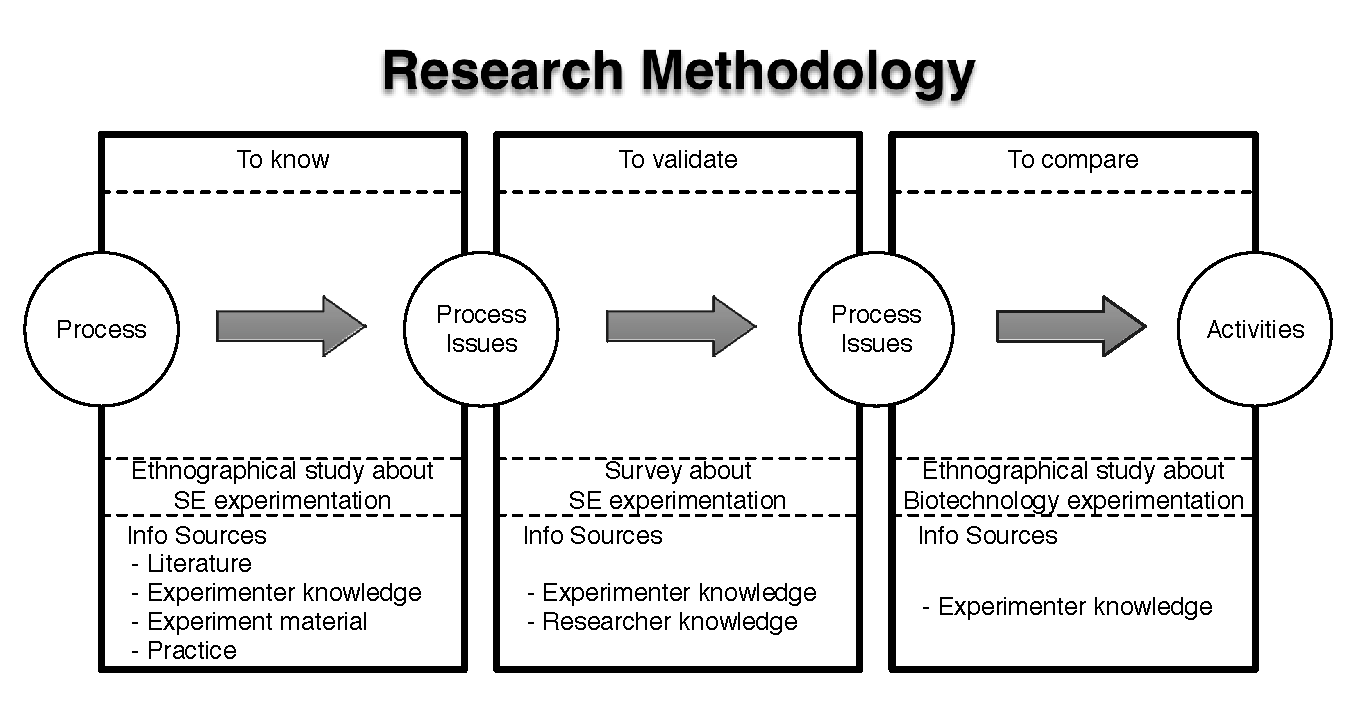
\includegraphics[width=12cm]{Images/Methodology}
	\caption{Research Methodology}
	\label{fig-research-methodology}
\end{figure*}

Cada una de las fases de investigaci�n fue guiada por un objetivo espec�fico, los cuales se listan a continuaci�n.

\begin{framed}%
%\textbf{SG2: How do researchers conduct SE experiments in practice?}
\textbf{SG1: To identify how researchers conduct SE experiments in practice into a specific research group}
\end{framed}

\begin{framed}%
%\textbf{SG1: How generalizable is the experimentation process performed into a specific SE research group?}
\textbf{SG2: To determine the generalizability of the experimentation process performed into a specific SE research group}
\end{framed}

\begin{framed}%
%\textbf{SG3: Does SE experimentation practice deviate from traditional disciplines?}
\textbf{SG3: To verify whether there is deviation of SE experimentation practice from traditional disciplines}
\end{framed}

In order to answer the research questions a mixed research methodology was applied. First, we conducted an ethnographical study to observe how a representative SE research group: Natalia Juristo's team (GrISE) at the Universidad Polit�cnica de Madrid (Spain) works. Since the results obtained from a unique research group are not necessarily generalizable, and the lack of depth in certain controversial aspects identified in GrISE, we performed a survey in order to strengthen our findings and extrapolating it to the ESE community. Finally, another ethnographical study was carried out in different representative research groups of Biotechnology at the Universidad de las Fuerzas Armadas ESPE (Ecuador). The aim of this second study was to compare SE experimentation in practice with that of another traditional discipline.

\subsection{Design of ethnographical studies}
Dar respuesta a RQ1 y RQ3 representa un gran desaf�o de investigaci�n, dado que supone el estudio de fuentes de informaci�n disponibles de un n�mero representativo de grupos de investigaci�n en ESE y en Biotecnolog�a, tal que se pueda conocer a detalle los retos que enfrenta el experimentador antes durante y despu�s de realizar las tareas de experimentaci�n en la pr�ctica. Todo esto, de la mano con el protocolo experimental descrito de forma te�rica en varias fuentes espec�ficas, tales como: textos, gu�as, manuales t�cnicos, reportes experimentales, entre otros.

Sin embargo, se torna muy complejo o casi imposible, realizar la investigaci�n en varias muestras del universo de grupos de investigaci�n de ambas disciplinas, dado el alto costo que esto representa (es decir, bloquear y controlar variables en los grupos, excesivo tiempo de investigaci�n en cada grupo, disponibilidad limitada de grupos afines para llevar a cabo la investigaci�n, disponibilidad limitada del tiempo de los experimentadores para con la investigaci�n, entre otros).

Esta situaci�n limita a que la investigaci�n sea llevada a cabo en un m�nimo n�mero de grupos de investigaci�n, lo que implica ciertos riesgos, dado que la validez de los resultados se ve amenazada. Para disminuir estos riesgos, creemos que los resultados deben responder a un riguroso proceso investigativo, los contextos de experimentaci�n seleccionados debe ser muy representativos en la poblaci�n bajo estudio y deben ser validados por otro medio los resultados obtenidos.

Visto desde esta perspectiva, se precisa aplicar una aproximaci�n emp�rica de observaci�n con alg�n tipo de interacci�n cuyo protocolo de investigaci�n se alinee con la naturaleza de la problem�tica identificada para garantizar la fiabilidad de los resultados obtenidos, enfatizar las caracter�sticas de la investigaci�n, su validez y significancia cient�fica \cite{sjoberg-2007-future-empical-methods}. Por lo tanto, los m�todos factibles a ser utilizados eran: etnograf�a, action research o case study.

En esta investigaci�n se necesitaba estudiar como se desarrolla un fen�meno (experimentaci�n) en su entorno natural (grupos de investigaci�n), por lo que realizamos an ethnographical study [REF].

\subsubsection{Context selection}
El criterio de selecci�n aplicado en los estudios etnogr�ficos parte de la premisa que un grupo de investigaci�n representativo representa una fuente fiable de informaci�n, lo que facilitar�a la tarea de aprendizaje respecto a la experimentaci�n. Por lo tanto, el criterio de selecci�n responde a las siguientes condiciones:

\begin{itemize}
\item{Ser un grupo de investigaci�n cuyos experimentadores tengan una consolidada experiencia den el �rea}

\item{Ser un grupo de investigaci�n cuyos experimentadores sean reconocidos en la comunidad cient�fica a trav�s de publicaciones de alto impacto, tales como libros, art�culos, manuales t�cnicos, entre otras.)}
\end{itemize}

%%%%%%%%%%%%%
%HASTA AQUI
%%%%%%%%%%%%%

Dadas las condiciones, los grupos de investigaci�n seleccionados son, por una parte, el Grupo GrISE perteneciente a la Escuela T�cnica Superior de Ingenieros Inform�ticos (ETSII) de la UPM de Espa�a y por otra parte, el �rea de Biotecnolog�a de Grupo de Investigaci�n en Modelos de Producci�n de Software (GrIMPSoft) perteneciente al Departamento de Ciencias de la Computaci�n (DECC) de la ESPE de Ecuador. Una descripci�n detallada de los grupos de investigaci�n seleccionados se realiza en las Secciones \ref{sec-execution-1} y \ref{sec-execution-2}, respectivamente.

\subsubsection{Data collection procedure(s)}\label{subsec-data-collection}
El proceso de recolecci�n de informaci�n que ser� aplicado consiste en un ciclo iterativo incremental de acciones realizadas sobre distintas fuentes de informaci�n (ver Figura \ref{fig-proceso-investigacion}), con el prop�sito de indagar sobre la experimentaci�n llevada a cabo en grupos de investigaci�n de distintas disciplinas.

\begin{figure}[htbp!]
	\centering
	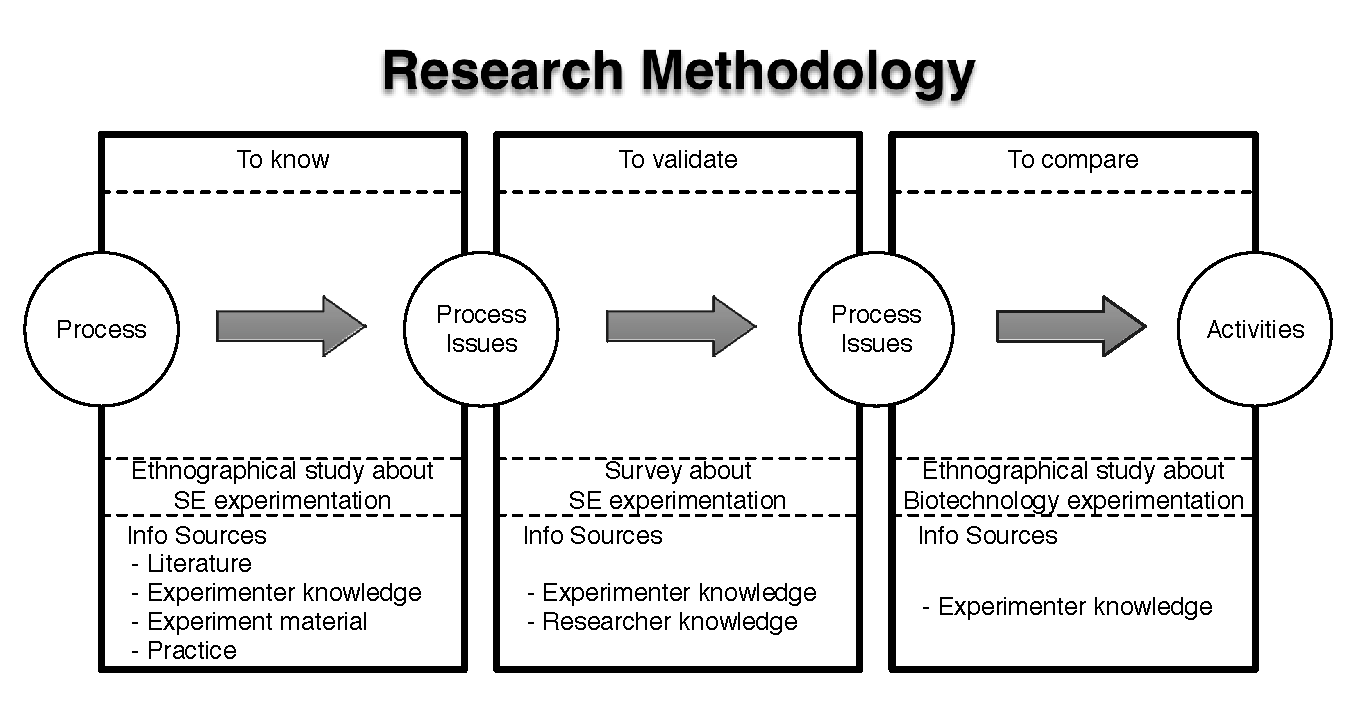
\includegraphics[width=3.5in]{Images/Methodology}
	\caption{Research Methodology}
	\centering
	\label{fig-research-methodology}
\end{figure}

Las fuentes generadoras de informaci�n corresponden espec�ficamente a aquellas que son accesibles y representativas dentro del grupo de investigaci�n bajo estudio. Para la presente investigaci�n se considera a la: Literatura com�n del grupo (general y espec�fica), material experimental del grupo (general y espec�fico) y conocimiento de los experimentadores del grupo (internos y externos).

El orden en el que el investigador tomar� contacto con las fuentes generadoras de informaci�n ser� aleatorio. La frecuencia de contacto con las fuentes depender� de la necesidad del investigador por obtener conocimiento; pero sobre todo, depender� de la disponibilidad de cada fuente. Es decir, mientras m�s disponible sea la fuente, el investigador podr� estar m�s tiempo en contacto con la misma. A continuaci�n se detalla la interacci�n que mantendr� el investigador con cada fuente.

\begin{itemize}
  \item En lo que respecta a la literatura com�n del grupo, el investigador tendr� acceso a la misma de forma inmediata y continua en el tiempo, a trav�s de distintos medios (por ejemplo: bibliotecas, bases digitales disponibles, versiones impresas disponibles, entre otras). La literatura representa una fuente de informaci�n muy importante, dado que proporcionar� la informaci�n referente al proceso de experimentaci�n, desde la perspectiva te�rica.
 
  \item El contacto con el material experimental m�s representativo y fiable propio del grupo de investigaci�n ser� inmediato y continuo en el tiempo, con la gu�a de los experimentadores. Sin embargo, para facilitar el proceso de revisi�n y aprendizaje de la informaci�n contenida en esta fuente, se precisar� un contacto previo con la literatura com�n del grupo. Eventualmente ser� preciso el estudio de material espec�fico para profundizar en una tem�tica particular. El material experimental representar� la evidencia de la experimentaci�n llevada a cabo en la pr�ctica por el grupo de investigaci�n.

  \item La obtenci�n del conocimiento de los experimentadores ser� planificada en funci�n de su disponibilidad de tiempo. Este proceso se realizar� desde un inicio, ya que se prev� una alta complejidad, considerando la aplicaci�n de distintas t�cnicas e instrumentos. Para el caso de los experimentadores externos, no ser� posible una planificaci�n espec�fica, dada la dificultad de un contacto directo; por lo tanto, en este punto mucho se depender� de la casualidad. El conocimiento obtenido de los experimentadores, representar� el proceso de experimentaci�n realizado en la practica dentro de los grupos de investigaci�n. 
\end{itemize}

Se prev� que el conocimiento obtenido de las fuentes indicadas se complementar�n entre si y servir� para determinar en qu� medida lo que que se encuentra expresado en la teor�a, corresponde a lo que efectivamente llevan a cabo los experimentadores en la pr�ctica dentro de los grupos de investigaci�n.

Para el proceso de extracci�n de la informaci�n se utilizar� una taxonom�a de t�cnicas de recolecci�n de informaci�n, categorizada de acuerdo al nivel de contacto con la fuente primaria de informaci�n, en este caso los experimentadores de cada entorno. La taxonom�a propone tres niveles de recolecci�n de informaci�n: Participaci�n directa con la fuente (nivel 1), participaci�n indirecta con la fuente (nivel 2) y estudio del material de trabajo (sin la participaci�n de la fuente) (nivel 3) \cite{Lethbridge-2005-studyingsoftwaredatacollection}.

El procedimiento para la recolecci�n de informaci�n de las fuentes indicadas, consiste en aplicar t�cnicas adecuadas dependiendo del tipo de fuente y de su disponibilidad. Por ejemplo, para extraer informaci�n de los experimentadores de un entorno de experimentaci�n se utilizar�n t�cnica t�cnicas tales como: entrevistas, grupos de discusi�n, entre otros (primer nivel). La adecuada aplicaci�n de las t�cnicas de recolecci�n de informaci�n estar� asociada a la utilizaci�n de diferentes instrumentos, algunos de los cuales se constituir�n como piezas fundamentales para recrear la informaci�n obtenida. Por ejemplo utilizaremos: videoc�maras, dispositivos de grabaci�n de audio, entre otros. M�s espec�ficamente, las t�cnicas de recolecci�n de informaci�n que se aplicar�n a las fuentes de informaci�n, se indican en la Tabla \ref{tbl-tecnica-fuente}.

\begin{table}
	\centering
	\caption{T�cnicas de recolecci�n por fuente de informaci�n}
	\label{tbl-tecnica-fuente}
	\begin{tabular}{|p{3cm}|p{3.7cm}|}
	\hline
	\textbf{Fuente} & \textbf{T�cnicas}\\
	\hline
	\multirow{7}{50 pt}{Conocimiento del grupo de investigaci�n} & Entrevistas\\
	\cline{2-2}
	& Grupos de discusi�n\\
	\cline{2-2}
	& Observaci�n participativa\\
	\cline{2-2}
	& Modelado de actividades\\
	\cline{2-2}
	& Sistemas instrumentales\\
	\cline{2-2}
	& Aprendizaje basado la experiencia\\
	\hline
	\multirow{1}{75 pt}{Literatura referente} & An�lisis de documentaci�n\\
	\hline
	\multirow{1}{75 pt}{Material experimental} & An�lisis de documentaci�n\\
	\hline
	\multirow{4}{50 pt}{Conocimiento de experimentadores externos} & Entrevistas\\
	\cline{2-2}
	& Grupos de discusi�n\\
	\cline{2-2}
	& Sistemas instrumentales\\
	&\\
	\hline
	\end{tabular}
\end{table}
 
Los inconvenientes presentados por el uso de las diferentes t�cnicas e instrumentos, ser�n minimizados gracias a su combinaci�n en cada iteraci�n. Por ejemplo, los vac�os del audio podr�n ser complementados por el video, las fotograf�as y los esbozos de los experimentadores y viceversa.

\subsubsection{Data analysis procedure(s)}
El procedimiento de an�lisis de datos tendr� un enfoque cualitativo y estar� asociado con la aplicaci�n de las t�cnicas de obtenci�n de informaci�n. Por lo tanto, este procedimiento tambi�n ser� de tipo iterativo incremental. El n�mero de iteraciones de an�lisis corresponder� al n�mero de iteraciones de recolecci�n de datos realizado con cada fuente. El procedimiento de an�lisis (ver Figura \ref{fig-proc-analisis}) se compone de dos actividades principales: (1) Verificaci�n de los datos y (2) Comparaci�n de los datos.

\begin{figure}[htbp!]
	\centering
	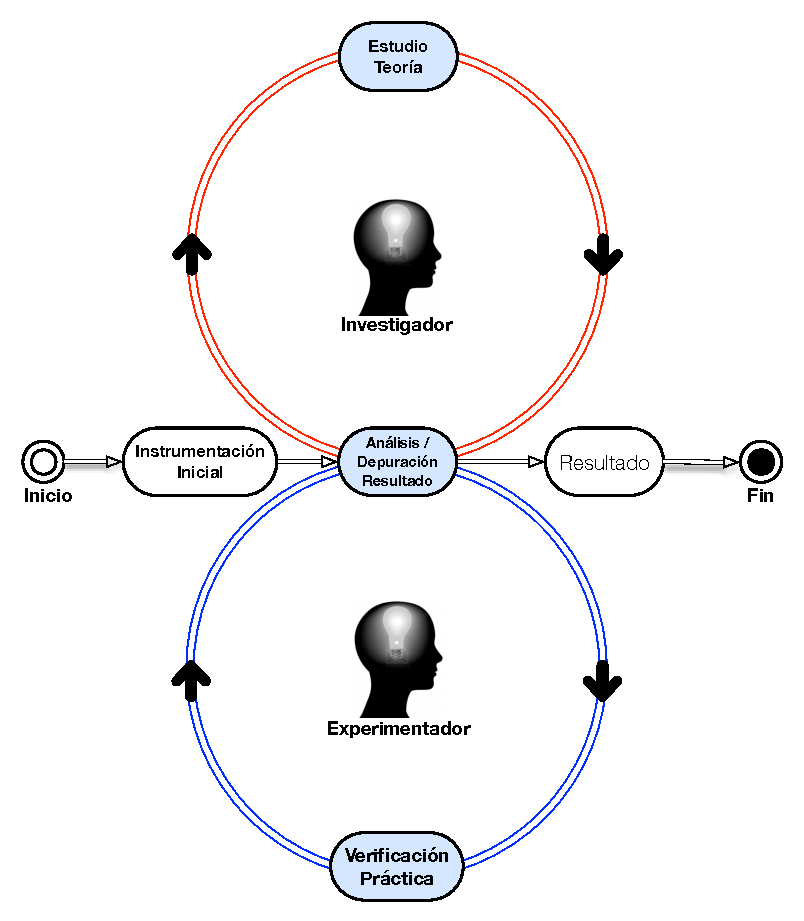
\includegraphics[width=2.5in]{Images/proceso-analisis}
	\caption{Proceso de An�lisis}
	\label{fig-proc-analisis}
\end{figure}

\begin{enumerate}[(a)]
\item \textbf{Verificaci�n de los datos: }Esta actividad tiene como objetivo verificar la validez de la informaci�n recolectada como insumo para el an�lisis, lo cual ser� realizado principalmente por los experimentadores del grupo. Durante las revisiones de las fuentes te�ricas, el investigador ir� adquiriendo paulatinamente conocimientos b�sicos de la experimentaci�n, lo cual le servir� para entender m�s f�cilmente los resultados obtenidos de la interacci�n con el conocimiento de los experimentadores. Estos resultados ser�n expresados de forma expl�cita en medios f�sicos o digitales y validados por el experimentador en cada iteraci�n hasta obtener el resultado final.
 
\item \textbf{Comparaci�n de los datos: } La comparaci�n de los datos obtenidos ser� realizada tanto por el investigador como por el experimentador, en una actividad de revisi�n cruzada, cada vez que hacen la verificaci�n de los datos en los resultados intermedios obtenidos. Por un lado el investigador hace la comparaci�n del resultado con su conocimiento adquirido de la revisi�n de otras fuentes de informaci�n; mientras que el experimentador compara el resultado con las actividades que efectivamente realiza en la pr�ctica. Una vez valida la informaci�n recabada el proceso de an�lisis concluye.
\end{enumerate}

\subsection{Survey of the experimentation process in SE}
y por otra parte, validaremos los hallazgos del proceso de etnograf�a en la comunidad de ESE a trav�s de un survey. Siguiendo los lineamientos propuestos por Runenson et al. \cite{case-study-in-SE-Runenson-2012} a continuaci�n detallamos: (1) El objetivo de la investigaci�n, (2) La descripci�n del procedimiento de selecci�n el caso, (3) el procedimiento de recolecci�n de datos y (4) Los procedimientos de validaci�n del estudio.

\section{Experimentation in software engineering}\label{sec-ESE-etnography}
\odnote{Tendremos que discutir con Natalia si debemos hacer an�nimos los grupos. Teniendo en cuenta lo que se dice, creo que es justificable. Una aproximaci�n posible es hacer que los grupos sean conocidos para los revisores, pero no para los lectores.}
\rodrinote{No me queda claro c�mo hacer que los grupos sean conocidos para los revisores y no para los lectores, ya me lo dir�s.}

El estudio fue realizado en el Grupo de Investigaci�n en Ingenier�a de Software Experimental (GrISE) de la Universidad Polit�cnica de Madrid (UPM). GrISE es un grupo que puede considerarse representativo de la comunidad de ESE. El origen del grupo data de finales de los 90s, cuando fue fundado por N. Juristo, una investigadora reconocida en IS por su temprano libro (con A. Moreno) acerca de SE experimental \cite{Juristo2001}, adem�s de sus contribuciones posteriores. El grupo cuenta con otros investigadores de dilatada trayectoria, tales como O. Dieste y S. Vegas. A lo largo de su historia, GrISE ha realizado varias familias de experimentos \cite{Basili1999-KnowledgeFamiliesExp}, en distintas tem�ticas: testing (�ntimamente relacionada con los experimentos iniciados por Basili y colaboradores, tales como \cite{Juristo-2012-Effectiveness-Testing}), requisitos (\cite{Aranda-2014-Bias-Family-Experiments}) y, m�s recientemente, test-driven development (e.g., \cite{Tosun-2017-experiment-TDD}). Con el prop�sito de evitar confusi�n en el lector, creemos preciso indicar que de aqu� en m�s nos referiremos como \textquotedblleft los investigadores\textquotedblright a quienes llevamos a cabo la presente investigaci�n; y como \textquotedblleft los experimentadores\textquotedblright a los investigadores que fueron objeto de estudio.

El estudio se desarroll� por fases iteradas, tal y como se puede observar en la Figura \ref{fig-process-etnography-study1}. Las fases no fueron planificadas de antemano, sino que se plantearon sobre la base de los hallazgos obtenidos durante la investigaci�n, tal y como detallaremos a lo largo de esta secci�n. La descripci�n tendr� un car�cter denso\footnote{A 'dense' or 'thick' description is a reporting style in ethnographic studies in which the research findings are explicitly related to their occurring context. A dense description facilitates the critical evaluation of the findings, e.g., their external validity, by enabling the comparison to other contexts. For instance, see \cite[pp. 60-62]{Outhwaite-2007-SAGE-Handbook}}, tal y como es habitual en Etnograf�a. El lector encontrar� fragmentos subrayados; dichos fragmentos representan, en nuestra opini�n, hallazgos importantes de la investigaci�n etnogr�fica. Dichos hallazgos se recopilan y discuten en la Secci�n~\ref{sec-discussion-conclusions}. La totalidad de los datos recogidos durante el trabajo de campo obedece a un compendio de fotograf�as, grabaciones de audio, v�deos, y reportes; los cuales se encuentran disponibles en este \href{http://190.15.140.14/erfonseca/productos-intermedios/resolucion/etapa1/accion1/}{\underline{\textit{sitio}}}.

\begin{figure}[htbp!]
	\centering
	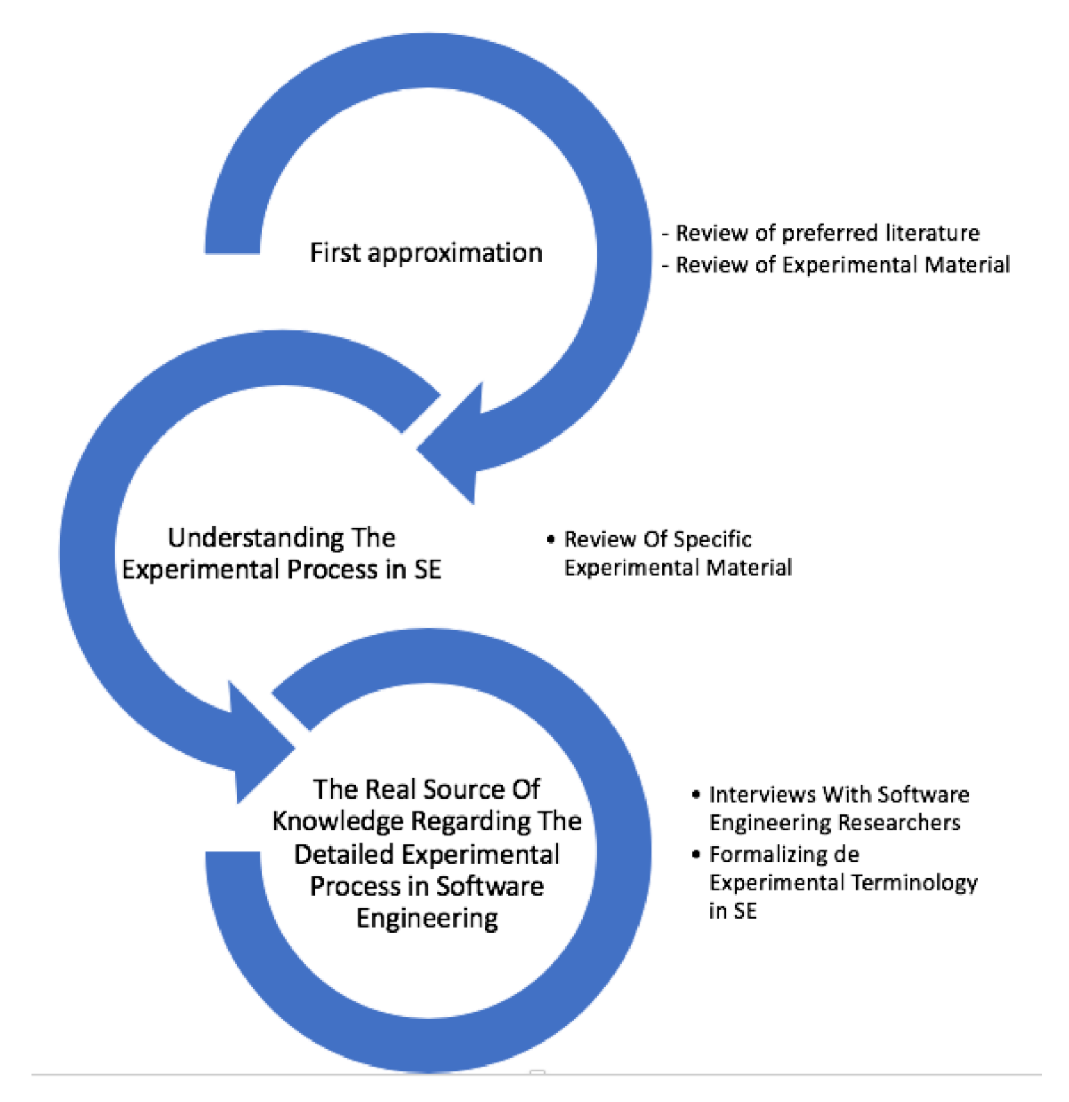
\includegraphics[width=3.2in]{images/Etnogaphy1-Process}
	\caption{Fases del Estudio Etnogr�fico de la Experimentaci�n en SE}
	\label{fig-process-etnography-study1}
\end{figure}

\subsection{First Approximation}\label{subsec-results-case1}
Las primeras actividades realizadas fueron entrevistas y grupos de discusi�n con los miembros del GrISE. El objetivo de estas actividades fue adquirir el conocimiento del grupo y volcarlo en modelos que permitiesen su an�lisis y manipulaci�n posterior. Con esto pretendimos hacer expl�cito el conocimiento de los experimentadores sobre experimentaci�n en SE; as� como tambi�n, formalizar en consenso el resultado obtenido \cite{Biffl-2013-Replication-Data-Management}. Realizamos varias entrevistas a experimentadores de distintos perfiles en el �rea de la experimentaci�n en IS, tales como: experimentadores de dilatada experiencia (2), experimentadores con mediana experiencia (2) y experimentadores novatos (2). 

%\odnote{RODRIGO: Y para qu� obtenemos los modelos conceptuales? HAY QUE DECIRLO. probablemente debemos referenciar \url{https://ieeexplore.ieee.org/document/6681356}. Son para una investigaci�n distinta. Deber�amos ponerlos directamente en un anexo web compartido con otra potencial publicaci�n en modelado de experimentos, que surja como resultado de la etnograf�a + SLR? Yo creo que es la mejor opci�n. Por lo de pronto, podemos ir poniendo los modelos en el anexo del paper, y antes de submitir el paper moverlos a internet.}

Pronto se evidenci� que las actividades realizadas iban a ser insuficientes para alcanzar este objetivo. Los miembros del GrISE nos proporcionaron cierto conocimiento expl�cito referido particularmente a los componentes principales de un experimento (hip�tesis, factor, nivel, etc.). Sin embargo, en un principio no result� posible profundizar demasiado:

\begin{itemize}
	\item Algunos miembros del GrISE cre�an que las actividades realizadas eran innecesarias, ya que el conocimiento que busc�bamos pod�amos adquirirlo por nosotros mismos en la {\color{blue}(?)} \ul{literatura que ellos consideraban est�ndar}, e.g., \cite{Wohlin2000}.
	\item A medida que profundiz�bamos en algunas �reas, e.g., planificaci�n experimental o gesti�n de datos, los miembros del GrISE necesitaban {\color{blue}(?)} \ul{apoyar su relato con ejemplos concretos}, que obten�an de su propio material experimental, lo que dificultaba la comunicaci�n, ya que nosotros desconoc�amos dichos materiales.
	\item Los investigadores en un inicio no ten�an el nivel de conocimiento necesario para entender f�cilmente el relato y las discusiones de los experimentadores.
\end{itemize}

El estudio en paralelo de ambas fuentes (literatura relacionada y material experimental) result� imprescindible para proseguir la interacci�n con los miembros del GrISE. El modo en que el estudio fue realizado y los hallazgos del mismo se describen en las secciones siguientes.

\subsubsection{An�lisis de la literatura relevante}\label{subsubsec-study-literature}
Los miembros del GrISE se�alaron como {\color{blue}(39)} \ul{fuentes b�sicas de su proceso experimental los libros} by Wohlin et al. \cite{Wohlin2000} and Juristo \& Moreno \cite{Juristo2001}. En el GrISE tambi�n se {\color{blue}(40)} \ul{utilizan	 como fuentes b�sicas ciertos reportes o art�culos espec�ficos}. Resultan especialmente relevantes los textos de Basili et al. \cite{Basili-1986-ESE} y Kitchenham et al. \cite{Kitchenham2002-GuideLinesESE}, los cuales representan recomendaciones tempranas acerca de c�mo experimentar en SE. En el caso particular del GrISE, dado su inter�s por realizar replicaciones experimentales, resulta tambi�n especialmente relevante el trabajo de Basili et al. \cite{Basili1999-KnowledgeFamiliesExp}.

La literatura fue revisada en profundidad por los investigadores principales de este estudio (E. Fonseca y E. Espinosa). El primer aspecto que nos llam� la atenci�n fue la {\color{blue}(2)} \ul{diversidad terminol�gica con que las distintas fuentes se refer�an a actividades similares del proceso experimental}. Para nosotros, observadores sin conocimientos espec�ficos de experimentaci�n, la literatura parecer�a describir distintos tipos de experimentos, cada uno caracterizado por un proceso diferente. A modo de ejemplo, los materiales antes citados \cite{Wohlin2000,Juristo2001,Basili-1986-ESE,Kitchenham2002-GuideLinesESE} denominan las fases del proceso de experimentaci�n en SE de la siguiente manera:

\begin{itemize}
	\item Wohlin et al. \cite{Wohlin2000} \textquotedblleft proponen como fases del proceso experimental: Experiment idea, Experiment scoping, Experiment planning, Experiment operation, Analysis \& interpretation, Presentation \& package and Experiment report\textquotedblright.
	\item Juristo \& Moreno \cite{Juristo2001}: \textquotedblleft Objective Definition, Design, Execution and Analysis\textquotedblright.
	\item Basili et al. \cite{Basili-1986-ESE}: \textquotedblleft Definition, Planning, Operation, and Interpretation\textquotedblright.
	\item Kitchenham et al. \cite{Kitchenham2002-GuideLinesESE}: \textquotedblleft Experimental context, Experimental design, Conduct of the experiment and Data collection, Analysis, Presentation of results, and Interpretation of results\textquotedblright.
\end{itemize}

Aunque los autores definen estas fases en detalle, la coincidencia en t�rminos y descripci�n difiere de uno a otro autor. Una vez adquiridos los conocimientos acerca de experimentaci�n en SE es inmediato percibir las similitudes, pero a�n as� {\color{blue}(?)} \ul{no est� claro si los distintos autores est�n describiendo exactamente las mismas actividades}.

Hemos buscado libros de texto complementarios a \cite{Wohlin2000,Juristo2001}, con la intenci�n de verificar si la diversidad terminol�gica era un problema general, o estaba circunscrito a las fuentes recomendadas. S�lo hemos localizado la nueva edici�n del libro de Wohlin et al. \cite{Wohlin2012-Experimentation} sobre experimentaci�n, y los libros especializados de Runeson et al. \cite{case-study-in-SE-Runenson-2012} y Kitchenham et al. \cite{Kitchenham-2015-Literature-Review-Book}. Preguntados a este respecto, los miembros del GrISE nos se�alaron otras fuentes, tales como Box et al. \cite{Box2008}, Montgomery \& Runger \cite{montgomery-2010-applied-statistics} o Field \cite{Field-2013-Discovering-Statistics-SPSS}, pero en seguida nos aclararon que se trataban de libros orientados m�s al an�lisis estad�stico que a la planificaci�n y dise�o de experimentos. En consecuencia, creemos poder afirmar que la {\color{blue}(5)} \ul{carencia de textos de referencia} es un aspecto caracter�stico de la experimentaci�n en SE.

\subsubsection{Review of experimental material}\label{subsubsec-study-material}
El estudio del material experimental de GrISE constituy� una fuente de informaci�n valiosa, ya que refleja el conocimiento t�cito presente en el grupo, gestado durante m�s de una d�cada de experimentaci�n. El material es variado; se compone fundamentalmente de: planteamientos de experimentos, dise�os, instrumentos experimentales (e.g.: formularios de tareas experimentales, formularios de recogida de datos, gu�as), objetos experimentales (e.g.: programas con faltas sembradas, especificaciones de requisitos alteradas con anomal�as), raw data (e.g.: hojas de excel con datos de mediciones de tareas experimentales realizadas, bases de datos), material de entrenamiento (e.g.: manuales t�cnicos, presentaciones) y, finalmente, publicaciones (e.g.: \cite{Juristo2012-EffectivenessWithinOutsideScopeExperiment,Juristo2006-SoftwareTestingTechniques,Juristo-2003-ESERNET}).

El primer problema que nos encontramos fue el acceso al material experimental, dado que {\color{blue}(12)} \ul{no existe una pol�tica de gesti�n del material}. Un ejemplo paradigm�tico son los raw data. Encontramos raw data en distintos tipos de ficheros, correspondientes a distintas versiones, {\color{blue}(9)} \ul{cuya ubicaci�n y formato son conocidos �nicamente por la persona que los gestiona}. Lo mismo puede afirmarse de los restantes tipos de materiales, incluidas las publicaciones; de no existir librer�as digitales, algunas incluso podr�an no haber estado accesibles.

Fue preciso solicitar ayuda a los miembros del GrISE para acceder al material experimental, entender su estructura y evoluci�n temporal. Revisamos primero lo m�s antiguo, avanzando progresivamente hacia la actualidad. La revisi�n fue apoyada por el albacea de la informaci�n, cuyo relato sumado a la informaci�n obtenida del material revisado, nos permiti� descubrir que  {\color{blue}(10)} \ul{las actividades que generaron el material experimental han ido evolucionando y mejorando con el tiempo}. Creemos que ello podr�a deberse fundamentalmente a: (1) la mayor experiencia y conocimientos acerca de experimentaci�n que el grupo ha obtenido con el paso del tiempo y (2) la mayor exigencia de los comit�s de programas de revistas y congresos, los cuales tambi�n han mejorado su pericia progresivamente.

Otro aspecto que nos llam� la atenci�n en la revisi�n del material experimental, fue la escasa formalidad en el planteamiento de los experimentos. Los documentos del GrISE se caracterizan por {\color{blue}(14)} \ul{realizar una descripci�n general de las actividades a ser realizadas en el experimento, pero no proporcionan una gu�a clara sobre el orden de ejecuci�n y relaci�n entre actividades experimentales}. Por ejemplo, encontramos planteamientos de experimentos que inclu�an un dise�o experimental, mientras que otros no. Cuando el dise�o experimental estaba presente, no se acostumbraba a indicar su tipo, sino �nicamente su estructura y conformaci�n (e.g., la tabla presente en \cite[pp. 92]{Juristo2001}).

Ya hemos mencionado que GrISE ha realizado distintas familias de experimentos. La comparaci�n de los materiales relativos a distintas familias (e.g., testing vs. requirements) pose�an marcadas diferencias. Estas diferencias eran de dos tipos:

\begin{itemize}
	\item El procedimiento experimental depend�a en gran medida de la familia \odnote{RODRIGO: Podr�amos poner ejemplos de diferencias, quiz�s entre las familias de testing y requisitos? Mira la secci�n \ref{conduccion-replicacion} para que no repitamos el mismo argumento} \rodrinote{OSCAR: Quedamos en que esta parte la rellenes tu porque yo desconozco el experimento de requisitos}. Al parecer {\color{blue}(13)} \ul{existe una diversidad de aproximaciones y enfoques sobre la realizaci�n de experimentos}, dependiendo de la familia y el investigador que los plantee.
	\item Los materiales hac�an referencia a t�rminos totalmente diferentes a los identificados hasta el momento en la literatura, tales como: \textit{efecto del cansancio}, \textit{efecto del aprendizaje}, etc. Poniendo en contraste la literatura y el material experimental revisados, estaba claro que {\color{blue}(34)} \ul{los reportes sufr�an incluso mayor diversidad terminol�gica que los libros de referencia}. Dependiendo de la familia, encontramos definiciones similares usando t�rminos diferentes, los mismos t�rminos con definiciones diferentes, y t�rminos diferentes con definiciones diferentes referidas al mismo concepto. Por ejemplo, response variable and dependent variable; \textquotedblleft Experiment Design\textquotedblright~by Wohlin et al. \cite[pp. 93]{Wohlin2012-Experimentation}: \textquotedblleft A design of an experiment describes how the tests are organized and run\textquotedblright, and  \textquotedblleft Experimental Design\textquotedblright~by GrISE: \textquotedblleft ... aspects the experiment is to involve, what variables are to be taken into account, what data are to be observed in the experiment, etc.\textquotedblright.
\end{itemize}

Nuestro objetivo inicial, como ya hemos indicado anteriormente, era adquirir el conocimiento del grupo y volcarlo en modelos. Aunque la literatura no era coherente entre s�, el material experimental era complejo en su composici�n, y en un inicio los resultados las entrevistas no eran muy entendibles de experimentador a experimentador, conseguimos unificar la terminolog�a sobre experimentos en un modelo conceptual preliminar que se muestra en la Fig.~\ref{fig-conceptos-preliminar}(debido a su gran tama�o, la figura se ha incluido en el Ap�ndice~\ref{sec:annex-models-SE}). Este modelo preliminar de conceptos tales como: Experimento, Replicaci�n, S�ntesis, Hip�tesis, Variables, Dise�o Experimental, etc., que hoy podr�amos decir que es de muy alto nivel de abstracci�n, fue suficiente en aquel entonces para continuar con la investigaci�n etnogr�fica; de hecho, este modelo se constituy� como el punto de partida y objeto de estudio de los grupos de discusi�n con los miembros del GrISE. Las entrevistas por su parte, estuvieron m�s enfocadas a las actividades que realizan los experimentadores en la pr�ctica. El detalle de estas dos actividades se indica m�s adelante.

La interacci�n con las fuentes citadas en sus distintas instancias empezaron a dar sus frutos en los investigadores, tal es as� que nos motivamos a vivir la experimentaci�n en la pr�ctica.

\subsection{Understanding the experimental process in SE}\label{subsec-second-aprox}
Un aspecto diferencial de la etnograf�a frente a otras metodolog�as de investigaci�n cualitativas es la \textit{observaci�n participativa}. Los investigadores etnogr�ficos deben adoptar "el punto de vista de los nativos" para entender mejor el motivo de sus acciones \cite[pp. 55-56]{outhwaite-2007-sage}. En nuestro caso, la incertidumbre surg�a de la diversidad terminol�gica y operativa observada en los materiales experimentales. En consecuencia, nos planteamos realizar nosotros mismos un experimento.

\subsubsection{Selecci�n del experimento}\label{seleccion-del-experimento}
En lugar de dise�ar un experimento desde el principio, nos pareci� preferible replicar un experimento previamente realizado por el GrISE. Hab�a dos motivos para ello:

\begin{itemize}
	\item Realizar una replicaci�n despertaba el inter�s de los miembros del GrISE, lo que nos aseguraba su colaboraci�n.
	\item La replicaci�n nos permitir�a recrear el dise�o, ejecuci�n, an�lisis y reporte de un experimento que hasta entonces s�lo hab�amos conocido mediante el examen de material escrito, lo que a su vez nos permitir�a entender mejor las motivaciones y decisiones tomadas en aquel entonces por los experimentadores.
\end{itemize}

The selected baseline experiment \cite{Juristo2012-EffectivenessWithinOutsideScopeExperiment} belongs to the testing family. La replicaci�n se llev� a cabo en la Universidad de la Fuerzas Armadas ESPE, Sede Latacunga (Ecuador), y fue publicada posteriormente \cite{Fonseca-2013-Replication-Efectiveness-In-Out}.

\subsubsection{Planificaci�n de la replicaci�n}\label{planificacion-replicacion}
Se ha indicado repetidas veces en la literatura la dificultad de realizar replicaciones experimentales \cite{Gallardo-2012-CG-PL-SE,Vegas-2006-communication-researchers,Miller2005,Gomez-2014-understanding-replication,DEMAGALHAES-2015-Replications-SE,Carver-2014-Replications-of-SE}. Los motivos aducidos son variados: Hay mucha incertidumbre sobre c�mo realizar las replicaciones de los experimentos de SE \cite{Gomez-2014-understanding-replication}, Dificultad de comunicaci�n entre los experimentadores \cite{Vegas-2006-communication-researchers}, es dif�cil obtener una configuraci�n que sea exactamente igual a la del experimento original \cite{Vegas-2006-communication-researchers}, la inmadurez del conocimiento de la SE experimental \cite{Gomez-2014-understanding-replication}, la disponibilidad de informaci�n sobre el estudio original \cite{Mende-2010-replication}, claridad en la definici�n y explicaci�n a los sujetos sobre de la terminolog�a utilizada \cite{Shull-2003-Replicated-SB}, presencia del conocimiento t�cito \cite{Shull2002-TacitKnoeledge}, entre otros. En nuestro caso, el principal problema fue {\color{blue}(14)} \ul{la carencia de una gu�a detallada de las actividades experimentales a realizar}, hecho que ya hab�amos observado anteriormente (en la Secci�n~\ref{subsubsec-study-material}).

Para planificar la replicaci�n, fue necesario contar con la participaci�n directa de los experimentadores que realizaron el experimento original (N. Juristo y S. Vegas), dado que nos result� complejo entender claramente la forma de realizar ciertas actividades del experimento. Por ejemplo, los detalles de como plantear el dise�o experimental y como aplicarlo en la pr�ctica. Los experimentadores nos dieron gu�as claves de como llevar a cabo dichas actividades experimentales, que no est�n hechas expl�citas en ninguna fuente de informaci�n. Su aporte principal fue \textit{guiar el dise�o experimental, el uso del material experimental y dar los lineamientos espec�ficos para realizar la ejecuci�n y an�lisis del experimento}{\color{blue}(28)}. 

\subsubsection{Conducci�n de la replicaci�n}\label{conduccion-replicacion}
La replicaci�n fue realizada por R. Fonseca. La gu�a proporcionada por N. Juristo y S. Vegas fue suficiente para comprender y ejecutar sin incidentes dignos de consideraci�n las distintas actividades del experimento. La existencia de materiales experimentales precisos (cuestionarios, descripciones de las tareas, programas, etc.) facilit� de sobremanera la realizaci�n del experimento, ya que todas los aspectos relevantes estaban definidos de antemano.

Los materiales experimentales no son siempre tan precisos como en el caso de la familia de testing. Como ya hemos reportado en la Secci�n~\ref{conduccion-replicacion}, los documentos de la familia de requisitos eran mucho menos detallados que los de la familia de testing. Seg�n nuestra experiencia con la replicaci�n de experimento de testing, dicha falta de detalle s�lo pod�a perjudicar la conducci�n del experimento. 

Los miembros del GrISE nos explicaron que el {\color{blue}(13.1)} \ul{tipo y nivel de detalle de los materiales experimentales estaba en relaci�n a las tareas que los sujetos deb�an realizar}. Por ejemplo, las preguntas que pueden surgir en un experimento en elicitaci�n mediante entrevistas son muy diversas, y no se puede preparar de antemano una respuesta para cada una de ellas. En contrapartida, en la familia de testing todos los sujetos realizaban m�s o menos la misma tarea de la misma forma, e.g., dise�o de casos de prueba mediante partici�n de equivalencia, lo que permit�a proporcionar a los sujetos materiales e instrucciones m�s precisos.

\subsubsection{Medici�n}\label{medicion-replicacion}
La medici�n de los resultados result� m�s complicada. La raw data del experimento se obten�a a partir de test cases propuestos por los sujetos experimentales. El problema fundamental era que los test cases no se ejecutaban, sino que los medidores (en este caso, R. Fonseca y E. Espinosa) evaluaban su capacidad para detectar una falta mediante la lectura e interpretaci�n de los mismos. Para completar la medici�n fue necesario consultar con los miembros del GrISE.

Este procedimiento nos pareci� en primera instancia discutible. Sin embargo, tras una discusi�n con S. Vegas, adquiri� pleno sentido; los casos de prueba generados por los sujetos pod�an ser incompletos/incorrectos, pero a�n as� se pod�a ensayar las condiciones de entrada adecuadas. Por este motivo, una evaluaci�n experta de los casos de prueba era m�s fair que su ejecuci�n. De nuevo, volv�amos a observar que {\color{blue}(13.2)} \ul{los procedimientos experimentales (en este caso la medici�n) depend�an fuertemente de la tarea experimental, las cuales dependen a su vez del �rea de investigaci�n}.

Los investigadores (E. Fonseca y E. Espinosa) obtuvieron la raw data por separado. Determinar si un caso de prueba detectaba o no una falta implicaba interpretar el caso de prueba, por lo que la decisi�n final ten�a un componente subjetivo. En una reuni�n posterior de consenso, se constat� diferencias entre la raw data obtenida por los dos investigadores. Las discrepancias pudieron ser resueltas, pero qued� de manifiesto que {\color{blue}(?)} \ul{la primera fase de la medici�n del experimento carec�a de sistematicidad}. 

Preguntados al respecto, los miembros del GrISE nos comentaron que era posible plantear procedimientos de medici�n m�s sistem�ticos, pero que {\color{blue}(?)} \ul{en general la incertidumbre en la medici�n no pod�a ser eliminada completamente}. A modo de ejemplo, en la familia de experimentos de TDD, la medici�n fue realizada usando casos de prueba automatizados. Sin embargo, el dise�o de los casos de prueba, el medidor, y el modo en que los casos de prueba se conectaban con el c�digo fuente pod�an generar fuertes discrepancias entre las mediciones. El problema de la sistematicidad de las mediciones no era exclusivo de SE, sino que tambi�n aparec�a en otras disciplinas como Psicolog�a, y en buena parte se deb�a al problema de que {\color{blue}(?)} \ul{en SE (como en Psicolog�a) trabajamos con constructos no observables (e.g., calidad) que se operacionalizan de modo no-est�ndar}, en lugar de m�tricas bien definidas como ocurre en otras �reas (e.g., longitud en F�sica).

En contrapartida, los restantes pasos de la medici�n (c�lculo de medidas a partir de la raw-data, y formateo de los datos para an�lisis) no implicaron incertidumbre alguna; pudimos reproducir con �xito los mismos ficheros usados en el baseline experiment \cite{Juristo2012-EffectivenessWithinOutsideScopeExperiment}.

\subsubsection{An�lisis y reporte}\label{analisis-reporte-replicacion}
C. Apa y O. Dieste (autores del paper \cite{Juristo2012-EffectivenessWithinOutsideScopeExperiment}, pero ninguno de ellos relacionados con la familia de experimentos de testing) proporcionaron soporte en el an�lisis y reporte de la replicaci�n. Ello fue necesario debido a que los investigadores (E. Fonseca y E. Espinosa) no pose�an en aquel momento formaci�n al respecto. 

En general, {\color{blue}(?)} \ul{tanto el an�lisis como el reporte fueron sencillos de realizar}. Por un lado, el dise�o experimental utilizado (\textit{cross-over}) estaba asociado a un m�todo de an�lisis bien definido (los detalles pueden consultarse en \cite{Vegas-2016-Crossover-Designs-ESE}). Por otra, exist�a un formato de reporte que el manuscrito deb�a seguir \cite{Carver2010-GuidelinesReplication}. Los miembros del GrISE nos aclararon que, con matices, {\color{blue}(?)} \ul{el an�lisis y reporte no suponen desaf�os sustanciales en SE}.

La �nica nota discordante fue, seg�n la percepci�n de los investigadores en aquel momento, la existencia de diferencias entre los resultados del baseline experiment y la replicaci�n. Siguiendo \cite{Juristo2009-DifRepESE}, intentamos buscar explicaciones basadas en el contexto experimental (e.g., tipos de sujetos, motivaci�n, etc.). No pudimos llegar a ninguna conclusi�n s�lida, pero el proceso de reflexi�n puso de manifiesto m�ltiples diferencias que, a nivel de grano fino, separaban el baseline experiment de la replicaci�n. Estas diferencias no s�lo implicaban a los sujetos experimentales, sino tambi�n a la formaci�n impartida de forma previa al experimento, organizaci�n y duraci�n de las sesiones experimentales, tipo de entrenamiento, diferencias dial�cticas remanentes en el material experimental, nivel de formaci�n de los sujetos. 

Estos aspectos de detalle no fueron tratados con suficiente extensi�n en las reuniones con los experimentadores originales, ni tampoco aparec�an descritos con suficiente detalle (y, en ocasiones, como es el caso de la formaci�n, no aparec�an descritos en absoluto) en los materiales experimentales. Independientemente de la ausencia de incidencias en la ejecuci�n de la replicaci�n, las diferencias observadas reafirmaron nuestra creencia de que, al menos en el caso del GrISE, {\color{blue}(29)} \ul{no existen gu�as claras que permita realizar una replicaci�n literal, externa e independiente del experimento original}. Como corolario,  {\color{blue}(?)} \ul{es necesaria la presencia de los experimentadores originales durante buena parte del proceso para que los resultados del baseline experiment y la replicaci�n sean comparables}\footnote{Esta observaci�n es independiente del valor de las replicaciones literales en la creaci�n de conocimiento, hecho discutido ampliamente en SE, e.g., \cite{}https://link.springer.com/article/10.1007\%2Fs10664-008-9061-0.}\rodrinote{OSCAR: En esta nota al pie hay un link que est� perdido o no es el correcto, por favor ind�came el art�culo que es para poner la referencia.}.

\subsubsection{Evaluaci�n de la observaci�n participativa}\label{evaluacion-observacion-participativa}
La experiencia de realizar una replicaci�n de un experimento fue positiva en general. Los investigadores aumentamos considerablemente nuestros conocimientos acerca de experimentar en SE, lo que a su vez nos permiti� comprobar la veracidad de hallazgos anteriores (e.g., el escaso detalle de los materiales experimentales) y realizar nuevos hallazgos (e.g., los problemas asociados a la medici�n de la raw data).

No obstante, el principal resultado de la observaci�n participativa ha sido el reconocimiento de {\color{blue}(8)} \ul{la existencia de un profundo conocimiento t�cito, particular de cada investigador}. El conocimiento t�cito se refleja de varios modos. Por una parte, ya hemos comentado la necesidad  de contar con la gu�a de los miembros del GrISE para realizar la replicaci�n experimental reportada en \cite{Fonseca-2013-Replication-Efectiveness-In-Out}. Sin embargo, quiz�s no hemos reiterado lo suficiente que dicha gu�a s�lo pod�a ser proporcionada por ciertos miembros de GrISE (N. Juristo y S. Vegas), pero no otros (e.g., O. Dieste). Lo mismo ocurr�a con la familia de experimentos de requisitos, s�lo que en este caso eran N. Juristo y O. Dieste estaban al corriente de los detalles. 

Por otra parte, la observaci�n participativa no permiti� mejorar de forma significativa el modelo conceptual mostrado en la Fig.~\ref{fig-conceptos-preliminar}. Apenas pudimos identificar unos pocos conceptos y relaciones, tal y como se observa en la Fig.~\ref{fig-conceptos-final-revision-fuentes}. No obstante, la presencia del conocimiento t�cito nos indic� el camino de la fuente m�s importante de informaci�n, el conocimiento de los experimentadores.

\subsection{Eliciting tacit knowledge}\label{subsec-conocimiento-grupo}
Como se pudo ver, la determinaci�n de los conceptos que participan en el proceso experimental est� en gran parte en manos de los experimentadores, dado que son quienes manipulan dichos conceptos para llevar a cabo la experimentaci�n. Los investigadores en este punto adquirimos conocimientos tales que en conjunto con los experimentadores, hemos obtenido la informaci�n b�sica para determinar los conceptos que participan en el ciclo experimental, ayudados de las herramientas m�s adecuadas. No obstante, El desaf�o inminente era obtener la mayor cantidad de conceptos del proceso experimental, terminolog�a, definici�n, etc., lo cual ha significado una dificultad, debido a la presencia del conocimiento t�cito tanto en los experimentadores como en los investigadores, ya que algunos conceptos son exclusivos del conocimiento de cada persona, a los cuales es complejo acceder (lo que \cite{Polanyi1996} llam� conocimiento t�cito de los experimentadores). As� mismo, ha ocurrido que en la especificaci�n de los conceptos del proceso experimental hubo desacuerdos entre los experimentadores con respecto a la terminolog�a utilizada, definiciones, etc.

\odnote{OSCAR: Habr�a que indicar algo al respecto del conocimiento adquirido por los investigadores, que les permite desde este momento interaccionar de tu a tu con los miembros de GRISE.}

Para la elicitaci�n del conocimiento t�cito, planificamos inicialmente una serie de entrevistas semi-estructuradas, basadas en un cuestionario orientado a obtener el detalle de las actividades que realiza cada miembro del GrISE dentro de cada una de las familias experimentales. Estas entrevistas tuvieron que ser complementadas con grupos de discusi�n, ya que debido a la diversidad terminol�gica y operativa presente en GrISE fue imposible alcanzar un grado de convergencia sustancial\footnote{Esto es notable, dado que GrISE es un grupo relativamente peque�o. Las razones m�s probables de este hecho son 1) el n�mero de familias experimentales activas en el grupo, y 2) la duraci�n de la investigaci�n dentro de cada familia, que se prolonga a lo largo de varios a�os y replicaciones.}. Los grupos de discusi�n aportaron mucho a la formalizaci�n conceptual, pero las entrevistas se enfocaron m�s al proceso de la experimentaci�n. Las siguientes secciones detallan las actividades realizadas.

\subsubsection{Semi-structured interviews}\label{subsubsec-interviews-ESE}
El cuestionario se bas� en preguntas abiertas, con el objetivo de motivar en el entrevistado un relato libre, pero relativamente ordenado, acerca de sus experiencias en la realizaci�n de experimentos en SE. Abandonamos la toma de notas, y pasamos a capturar en v�deo los detalles de la expresi�n verbal y gestual\footnote{Los videos realizados durante la investigaci�n est�n disponibles en \href{http://190.15.140.14/erfonseca/productos-intermedios/resolucion/etapa1/accion1/}{\underline{\textit{sitio}}}}. Recolectamos tambi�n los bocetos en papel (e.g., v�ase la Fig.~\ref{fig-proceso-exp-boseto}) con que los entrevistados apoyaban su discurso. Todo este material era analizado posteriormente siguiendo un proceso similar al de an�lisis de protocolos \cite{Pressley-1995-verbal-protocols}. En un inicio, por cada entrevista (incluidas todas sus sesiones) realizamos transcripciones de las grabaciones, lo que signific� un arduo trabajo. Finalmente, limitamos esta actividad �nicamente a las entrevistas de los experimentadores de mayor experiencia. La informaci�n obtenida de las entrevistas a los experimentadores de menor experiencia sirvi� a modo de referencia o validaci�n.

\begin{figure}[htbp!]
	\centering
	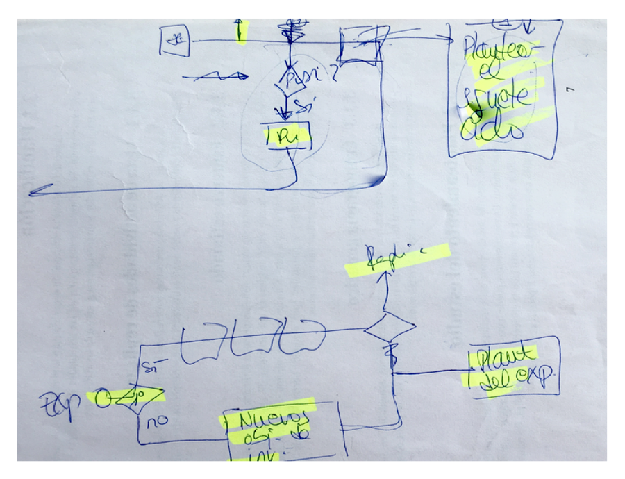
\includegraphics[width=3.2in]{images/Boseto-Proccess}
	\caption{Ejemplo de boceto confeccionado por los entrevistados.}
	\label{fig-proceso-exp-boseto}
\end{figure}

El conocimiento obtenido en cada sesi�n fue validado con el mismo entrevistado al inicio de una sesi�n posterior. En total, realizamos 7 entrevistas a 6 miembros de GrISE (un miembro relat� dos funciones distintas que realizaba en una familia de experimentos). Como se indic� anteriormente el nivel de conocimientos de los experimentadores entrevistados era diferente, por lo que la informaci�n que consideramos como base fue la obtenida de los experimentadores de mayor experiencia. El proceso en general no result� complejo, ya que cada entrevistado ofrec�a un relato coherente, quiz� porque todos ten�as los principios de la misma escuela. De este modo, las distintas iteraciones permitieron depurar progresivamente el conocimiento adquirido (e.g., v�ase la Fig.~\ref{fig-proceso-draft}) hasta un punto en el que progreso fue marginal, momento en el cual las entrevistas finalizaron. 

\begin{figure}[htbp!]
	\centering
	\includegraphics[width=3.2in]{images/Proccess-Draft}
	\caption{Extracto de las actividades experimentales realizadas por los experimentadores del GrISE (versi�n intermedia). La evoluci�n respecto a la Fig.~\ref{fig-proceso-exp-boseto} es claramente observable.}
	\label{fig-proceso-draft}
\end{figure}

El conocimiento adquirido se consolid� en tres productos: (a) Workflow del proceso de experimentaci�n en SE, (b) Modelo del proceso de experimentaci�n en SE, y (c) Documento descriptivo del proceso de experimentaci�n en SE.

El workflow del proceso se fue consolidando en las diferentes iteraciones de la entrevista a la investigadora de mayor experiencia (N. Juristo). Su origen se debe a que dicha investigadora opt� por explicar el proceso esbozando con papel y l�piz bocetos del workflow de la experimentaci�n en ingenier�a de software (e.g., v�ase la Fig.~\ref{fig-proceso-draft}). El workflow incluy� tambi�n elementos de las entrevistas de los otros experimentadores, lo que fue verificado y validado por N. Juristo. El modelo del workflow resultante (v�ase la Fig~\ref{fig-final-process-workflow}) muestra la secuencia de actividades a ser llevadas a cabo de principio a fin, en cada uno de los procesos principales del ciclo experimental.

El modelo del proceso se elabor� en paralelo y como complemento al workflow del proceso. La definici�n de este modelo fue propuesto por los investigadores, y tuvo como prop�sito definir la composici�n de procesos del ciclo de experimentaci�n en SE, haciendo analog�a con el proceso de desarrollo software. Esta forma de ver el ciclo experimental permiti� categorizar los procesos dentro del ciclo, a modo de una organizaci�n, as� como tambi�n permiti� identificar la participaci�n de roles en los diferentes procesos. El modelo del proceso tuvo una importante evoluci�n a la par del work flow (i.e.: en las distintas iteraciones de la entrevista con N. Juristo). El modelo del proceso obtenido (v�ase Fig.~\ref{fig-final-process-model}), muestra la interacci�n de los procesos necesarios para complementar el ciclo experimental, e indica los roles que ejecutan cada uno de los procesos; en resumen, define las categor�as de procesos de: apoyo, generaci�n de piezas del conocimiento, publicaciones, s�ntesis, b�sicos y organizativos. 

En cada sesi�n de las entrevistas, especialmente en las realizadas a los experimentadores de mayor experiencia, se gener� un documento basado en la transcripci�n de las grabaciones, pero con estructura y un plus del conocimiento de los investigadores. Cada experimentador fue verificando y validando el documento al inicio de cada nueva sesi�n. Al final del proceso de entrevistas se sintetiz� en un solo documento la informaci�n obtenida del proceso de experimentaci�n en SE.

La evoluci�n etnogr�fica de las piezas de conocimiento generadas en el proceso de entrevistas semi-estructuradas puede ser analizado accediendo a este \href{http://190.15.140.14/erfonseca/productos-intermedios/resolucion/etapa1/accion1/}{\underline{\textit{sitio}}}.

La observaci�n m�s relevante de esta fase de la investigaci�n etnogr�fica fue constatar que {\color{blue}(22)} \ul{los textos sobre experimentaci�n en SE existentes y el material experimental del grupo est�n lejos de mostrar el trabajo real que implica la experimentaci�n en la pr�ctica}. De hecho, tampoco los paquetes de laboratorio que se han encontrado en la literatura llegan al nivel de detalle de actividades y procesos que alcanzaron los productos obtenidos en las entrevistas (v�ase Figs.~\ref{fig-final-process-workflow} y \ref{fig-final-process-model}).

Por otra parte, las entrevistas pusieron de manifiesto que, al menos en GrISE, {\color{blue}(17)} \ul{ning�n experimentador lleva a cabo todas las actividades experimentales}. Parece que dentro de un grupo de investigaci�n {\color{blue}(31)} \ul{las responsabilidades se distribuyen en diversos roles} (que, obviamente, pueden ser desempe�ados por la misma persona o, como en el caso del GrISE, por personas distintas). Curiosamente, {\color{blue}(30)} \ul{no existe una asignaci�n explicita de roles a personas}; cada miembro de GrISE adoptaba un rol u otro dependiendo de la familia experimental. Por ejemplo, en la familia de experimentos de testing, una misma investigadora realiza el experimento en la pr�ctica y es la albacea de la informaci�n del experimento.

Dentro de GrISE, identificamos tres roles, a los cuales denominamos: (1) \textit{Research Manager}, (2) \textit{Experiment Manager} y (3) \textit{Senior Experimenter}. Estos roles no son necesariamente extrapolables a otros grupos de investigaci�n, pero parecen lo bastante bien definidos como para ser de car�cter general. Estos roles se encargaban de: (1) planificar la ejecuci�n del experimento, (2) ser el albacea de la informaci�n y (3) gestionar la log�stica de la experimentaci�n, respectivamente. Curiosamente, {\color{blue}(32)} \ul{existen actividades experimentales que son ejecutadas por distintos roles dentro de cada familia de experimentos}. Por ejemplo, la gesti�n de la replicaci�n experimental la realizan el \textit{Research Manager} y el \textit{Experimental Manager}. El planteamiento del experimento lo realizan el \textit{Research Manager} y el \textit{Senior Experimenter}. Esto denota una duplicaci�n de funciones, lo que posiblemente influya en la gesti�n del experimento. Se pudo percibir otros roles con un n�mero menor de actividades, los cuales eran asumidos por investigadores de menor experiencia; no obstante, no fueron considerados, ya que las actividades realizadas fueron contempladas en los roles principales.

En un inicio las entrevistas nos sirvieron, entre otras cosas, para consolidar nuestro conocimiento b�sico sobre experimentaci�n en SE, de la mano del an�lisis de la literatura relevante y la review of experimental material. Este conocimiento b�sico lo representamos, como ya se indic�, en un modelo conceptual inicial (v�ase la Fig.~\ref{fig-conceptos-preliminar}), el cual sirvi� como punto de partida para estructurar el modelo conceptual de la experimentaci�n en SE, para lo cual realizamos un proceso iterado de workshops.

\subsubsection{Workshops}\label{subsubsec-focus-groups}
Una vez iniciado el proceso de entrevistas individuales, realizamos una presentaci�n del modelo preliminar de conceptos de la experimentaci�n en SE a los miembros del GrISE. El resultado no pudo ser m�s calamitoso. La falta de acuerdo suger�a la realizaci�n de workshops para alcanzar un consenso o, al menos, poner de manifiesto el origen de las discrepancias. Las reuniones fueron guiadas generalmente por el miembro del GrISE con mayor experiencia. Cada reuni�n tuvo una duraci�n de al menos dos horas. Previo al inicio de las sesiones de discusi�n, cada miembro del GrISE analiz� en detalle el modelo base, sobre los que fueron haciendo aportes y modificaciones.  muy discutidas, pero finalmente al parecer consensuadas; siempre bajo la gu�a del moderador. 

Cada workshop causaba que el nivel de detalle de los modelos se incrementara considerablemente. Cada incremento se obten�a tras acaloradas discusiones que delataron la existencia de {\color{blue}(24)} \ul{diversidad terminol�gica incluso entre experimentadores que realizan actividades similares dentro de una misma familia experimental}. Por ejemplo, algunos experimentadores denominaban variable respuesta y otros variable dependiente al mismo concepto.

La raz�n de la diversidad terminol�gica entre experimentadores {\color{blue}(?)} \ul{parece deberse al tipo de formaci�n que cada experimentador ha recibido}. Hablar de~\textquotedblleft formaci�n\textquotedblright~en el contexto del GrISE es probablemente incorrecto. Todos los miembros de GrISE se han formado de forma autodidacta. Sin embargo, las fuentes que han utilizado para el estudio difieren (e.g., O. Dieste se ha formado en una tradici�n cercana a las ciencias de la salud, mientras que S. Vegas est� m�s pr�xima a la Ingenier�a).\odnote{RODRIGO: ser� esto cierto??} \rodrinote{OSCAR: No tengo idea} Dada que la terminolog�a en cada una de estas tradiciones difiere (e.g., treatment in medicine vs. level in engineering), la diversidad terminol�gica era una consecuencia inevitable. 

Tambi�n resulta interesante se�alar que la influencia de dichas tradiciones implica que la literatura preferida por el grupo (ver Secci�n~\ref{subsubsec-study-literature}) no representa la literatura \textit{realmente utilizada}. {\color{blue}(?)} \ul{Las fuentes utilizadas son, en realidad, m�ltiples, y su uso evoluciona con el tiempo}, e.g., el libro de Box et al. \cite{Box2008} ha sido reemplazado por \cite{Field-2013-Discovering-Statistics-SPSS} ya que proporciona una gu�a m�s detallada para realizar muchos an�lisis estad�sticos relevantes para el grupo.

A pesar de que aparentemente hubo consenso en en el modelo resultante (v�ase Fig.~\ref{fig-extract-final-concepts-model-no-consensus}), las acaloradas discusiones sobre los conceptos manejados y su definici�n, nos dieron pistas sobre una presunta desconformidad de algunos miembros, lo cual fue validado en las entrevistas personales que se llevaron en paralelo. El principal inconveniente argumentado por algunos miembros del GrISE sobre el modelo obtenido, fue respecto a la especialidad que tienen los miembros en fases espec�ficas del proceso, lo cual no estaba expresado en el modelo. Fue preciso entonces, iniciar un nuevo ciclo de discusiones grupales, con la particularidad de que cada experimentador expres� su conocimiento, �nicamente sobre los conceptos que maneja a trav�s de las actividades que efectivamente realiza en una instancia experimental. Este nuevo ciclo nos permiti� observar que \textit{los conceptos manejados por los experimentadores en SE obedecen a las actividades espec�ficas que realizan en una instancia experimental}{\color{blue}(18)}. Adicionalmente, se valid� \textit{la existencia de roles o perfiles de experimentadores: Experimentadores que custodian el material experimental del grupo, experimentadores que ejecutan en la pr�ctica la experimentaci�n y experimentadores que gestionan con el medio externo los nuevos experimentos y su factibilidad}{\color{blue}(33)}.

\begin{figure}[htbp!]
	\centering
	\includegraphics[width=3.4in]{images/Final-Concept-Model-No-Consensus}
	\caption{Extracto del Modelo Conceptual de la Experimentaci�n en GrISE (versi�n final sin consenso)}
	\label{fig-extract-final-concepts-model-no-consensus}
\end{figure}

\subsection{Conclusion}

Como resultado de este nuevo ciclo de discusiones obtuvimos tres modelos conceptuales (v�ase Figs.~\ref{fig-conceptual-model-RM}, \ref{fig-conceptual-model-EM}, y \ref{fig-conceptual-model-SE}), los cuales responden a los roles identificados durante el proceso de entrevistas.

Est� claro que el modelo base (ver Figura (ver Figura \ref{fig-conceptos-exp-boseto}) cambi� notablemente hasta llegar a aparente finales (v�ase Figs.~\ref{fig-conceptual-model-RM}, \ref{fig-conceptual-model-EM}, y \ref{fig-conceptual-model-SE}), \textit{los cual mostraron un amplio nivel de detalle conceptual, demostrando as� que el conocimiento m�s significativo de la experimentaci�n lo tienen los expertos}{\color{blue}(26)}. 

Los workshop representaron el punto final de la investigaci�n etnogr�fica. Esta investigaci�n represent� un periodo de observaci�n de 24 meses, tras los cuales identificamos una serie de caracter�sticas diferenciales de la experimentaci�n en SE. Los aspectos m�s destacados se han indicado (mediante un subrayado) a lo largo de la Secci�n~\ref{sec-ESE-etnography} y se resumen en la Secci�n~\ref{sec-discussion-conclusions}. Aplazaremos hasta dicha Secci�n la discusi�n de nuestros hallazgos, ya que tendremos la oportunidad de comparar las caracter�sticas de la experimentaci�n en SE con la situaci�n existente en una disciplina experimental asentada como la Biotecnolog�a. No obstante, algunos aspectos destacados pueden anticiparse aqu�:

\odnote{RODRIGO: La idea es que esta lista sirva como punto de conexi�n con el survey. NO est� terminada (avanzo hacia la etnograf�a de biotecnolog�a primero). Habr� que revisar la lista cuando el survey est� terminado. Tambi�n tendremos que comprobar que los subrayados pueden subsumirse (al menos en su mayor�a) en los items de la lista.}

\begin{itemize}

\item Los experimentadores se han educado en experimentaci�n de forma autodidacta. Aunque reconocen la existencia de ciertas obras de referencia en SE (e.g., \cite{Wohlin2000,Juristo2001}, las fuentes utilizadas son m�ltiples y evolucionan con el tiempo.

\item Existe de una gran diversidad terminol�gica, incluso entre investigadores que trabajan en la misma familia de experimentos. El car�cter autodidacta de la formaci�n y la diversidad de fuentes utilizadas explican esta diversidad.

\item Existe una amplia diversidad operativa, aunque restringida a las actividades de planificaci�n, dise�o y ejecuci�n de experimentos. La diversidad operativa puede deberse a: a) La diversidad de fuentes y b) lo distintos procedimientos que se aplican en �reas de investigaci�n distintas, e.g., testing vs. requirements. En contrapartida, el an�lisis y reporte son realizados de forma parecida por todos los experimentadores de GrISE.

\item La diversidad operativa se ve tambi�n favorecida por la escasa atenci�n que las fuentes en general prestan a estas actividades. Aunque el concepto de lab package existe desde hace tiempo, no parecen usarse en la pr�ctica. Los materiales experimentales no acostumbran a publicarse, a diferencia de los art�culos y an�lisis, por lo que tampoco se percibe la necesidad de una elaboraci�n cuidadosa de los mismos.

\item La diversidad terminol�gica y operativa dificulta la comunicaci�n entre experimentadores tanto dentro como fuera del grupo, y complica actividades b�sicas de investigaci�n, tales como la realizaci�n de replicaciones experimentales.

\item La comunicaci�n entre experimentadores se complica por la existencia de roles dentro de cada familia experimental, lo que provoca una compartimentalizaci�n del conocimiento e impide una convergencia terminol�gica y operativa. Ignoramos si este problema es particular del GrISE, debido a su reducido tama�o, o algo general independientemente del tama�o del grupo.

\item La existencia de roles y compartimentalizaci�n del conocimiento puede explicar igualmente la existencia de un voluminoso conocimiento t�cito.

\end{itemize}

Antes de progresar hacia el estudio etnogr�fico de la experimentaci�n en Biotecnolog�a, nos hemos preguntado cu�nto de generalizables son los hallazgos obtenidos en el grupo GrISE a la comunidad experimental de SE en general. Para averiguarlo, hemos realizado un survey, que reportamos en la siguiente Secci�n.


\section{Survey on Experimentation in Software Engineering}\label{sec-survey}
En base a los resultados del estudio entnogr�fico de la experimentaci�n en SE (Secci�n \ref{sec-methology}), nos preguntamos si la praxis del grupo de investigaci�n seleccionado coincide con la de la comunidad de ESE. M�s espec�ficamente, nos preguntamos si:

\begin{itemize}
	\item �Se ha formado la comunidad de ESE de modo similar al grupo de investigaci�n estudiado?
	\item �Son comunes los materiales de aprendizaje utilizados por la comunidad ESE y el grupo de investigaci�n estudiado?
	\item �Existe diversidad terminol�gica sobre experimentaci�n en la comunidad de ESE?
	\item �Existe diversidad operativa?
	\item �Existen roles asociados a la realizaci�n de tareas particulares?
\end{itemize}

El cuestionario planteado en el survey justamente se enfoc� en dar respuesta a estas interrogantes. La encuesta fue promovida durante the 2016 Empirical Software Engineering International Week (ESEIW) realizada en Ciudad Real (Spain). Este evento re�ne a los investigadores m�s emblem�ticos de la comunidad de ESE, y representa por lo tanto una poblaci�n adecuada para realizar el survey. La encuesta fue instrumentada a trav�s de Google Forms. 27 investigadores de diferentes partes del mundo participaron en el survey, lo que teniendo en consideraci�n los asistentes a la conferencia (112 personas, seg�n nos inform� la Conference Chair) supone un 24\% de response rate. Los investigadores de USA (4), Brazil (4) e Italia (3) son los que m�s representaci�n tuvieron (ver Fig. \ref{fig-nationality-respondents}), aunque obtuvimos respuestas de investigadores de 15 pa�ses.

\begin{figure}[htbp!]
	\centering
	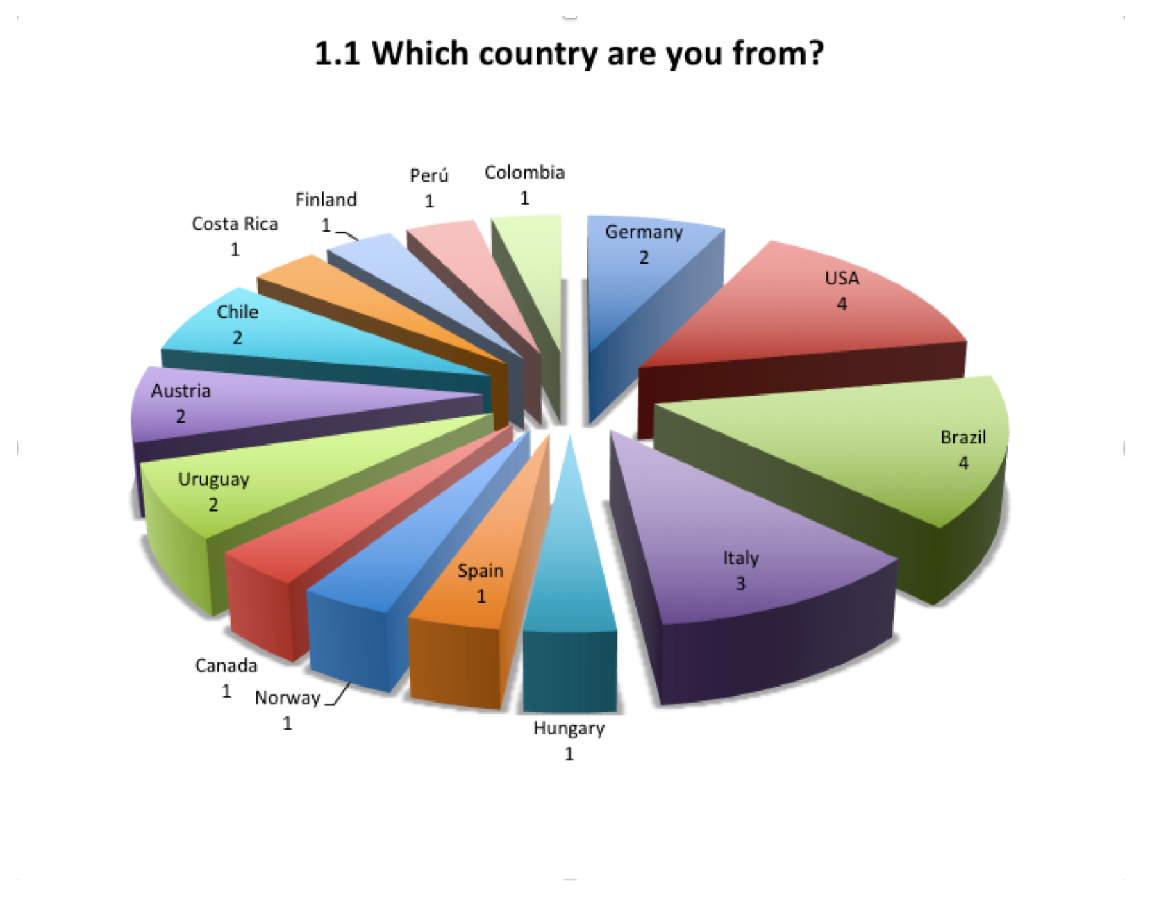
\includegraphics[width=3.4in]{Images/Nationality-respondents}
	\caption{Nationality of survey's respondents}
	\label{fig-nationality-respondents}
\end{figure}

Todos los participantes tienen un t�tulo en ciencias de la computaci�n. En su mayor�a son acad�micos (81.48\%). Muy pocos se identificaron como profesionales de la industria de software (7.41\%). La edad de la mayor�a de los participantes oscila entre 30-39 a�os (40.74\%) y los 40-49 a�os (37.04\%). Esto corrobora, si ello fuera necesario, la juventud de la experimentaci�n en SE.

Los experimentos controlados son el m�todo m�s com�nmente utilizado por los investigadores encuestados (66.67\%). Del 70\% de investigadores que han participado en la experimentaci�n en SE, un 22\% lo a hecho por m�s de 10 a�os, un n�mero similar entre 5 a 10 a�os, un 15\% por menos de dos a�os y un 11\% entre 2 a 5 a�os. Todo ello confirma que la poblaci�n seleccionada es adecuada para responder a las preguntas planteadas. Otros m�todos que tambi�n son aplicados habitualmente por los participantes son los cuasi-experimentos (44.44\%), seguidos de las encuestas (55.56\%) y los estudios de caso (48.15\%).

%\begin{figure*}[htbp!]
%	\centering
%	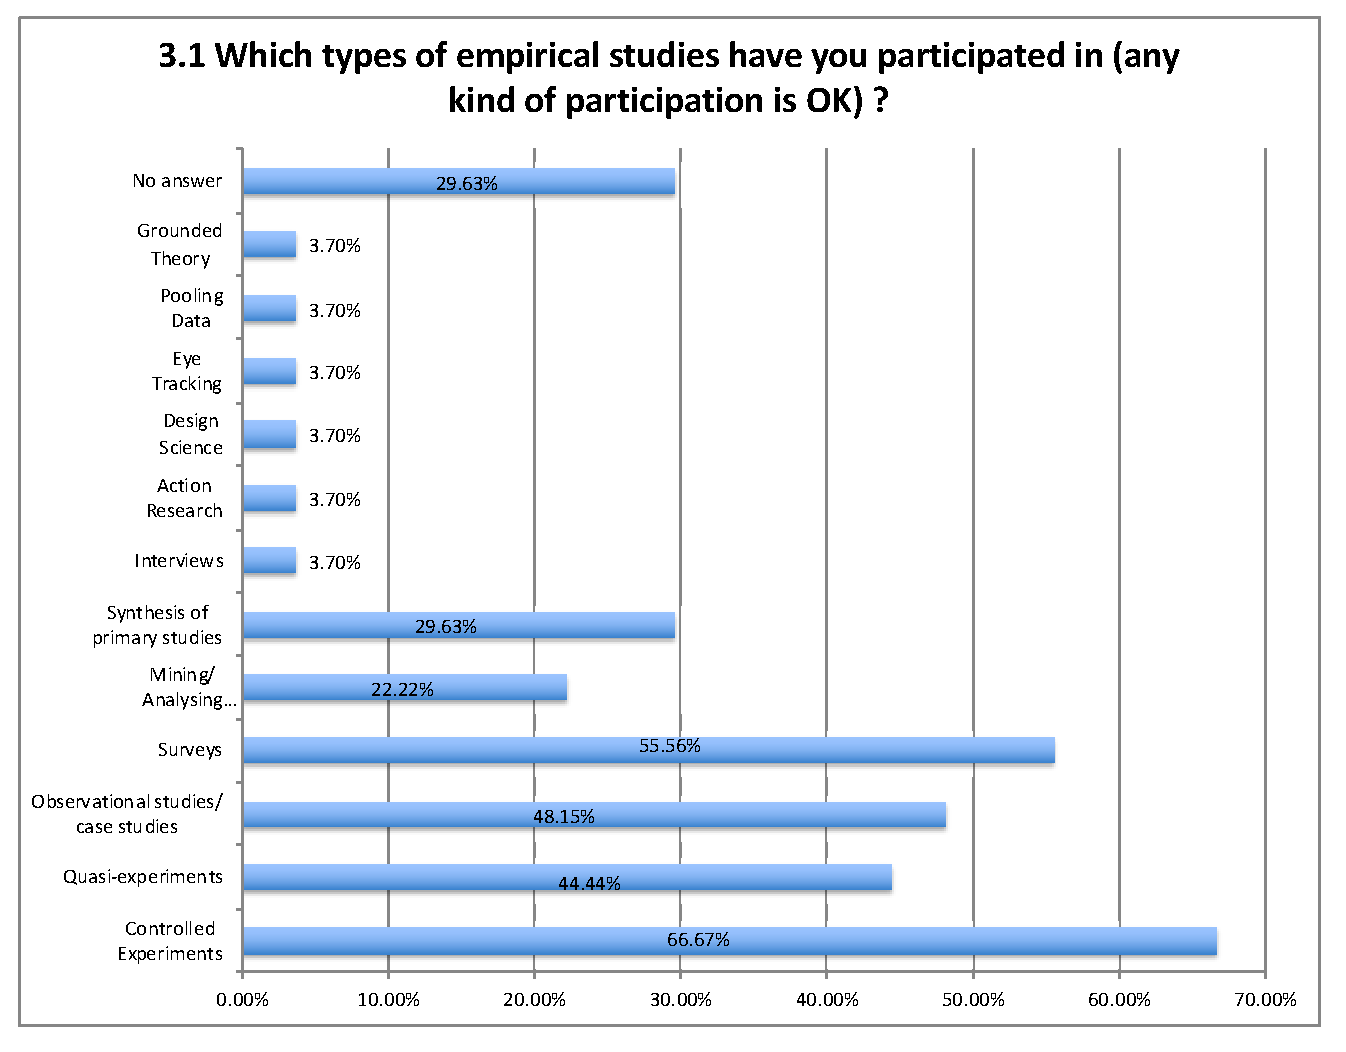
\includegraphics[width=10cm]{Images/Other-Empirical-Methods-SE}
%	\caption{Application of Other Empirical Methods in SE}
%	\label{fig-other-empirical-methods-SE}
%\end{figure*}

\subsection{Experimental training}
La mayor�a de los investigadores encuestados (66.67\%) indican que su formaci�n se bas� en la pr�ctica, y en el aprendizaje de la mano de investigadores con experiencia en el campo. Otras modalidades de formaci�n son cursos formales (59.26\%), auto aprendizaje a partir de textos de experimentaci�n (51.85\%) y de material experimental (48.15\%). El tiempo de formaci�n de los investigadores ha sido variado: el 26\% indican que se han formado al menos por un a�o, el  15\%  entre uno y dos a�os, y la mayor�a (59\%) por m�s de dos a�os. El panorama es bastante similar al observado en el grupo de investigaci�n estudiado; la formaci�n autodidacta es mayoritaria (SR1), y los tiempos de formaci�n son coincidentes, seg�n nos indican los investigadores del GrISE.

Abundando en el tema de la formaci�n de los investigadores, los t�picos abordados son variados. La Figura \ref{fig-topics-training} muestra las tem�ticas espec�ficas reportadas por los investigadores encuestados. Un 45\% de los investigadores coincidi� en haber estudiado el proceso de experimentaci�n, un 22\% indica haber estudiado m�todos emp�ricos tales como: experimentos controlados, replicaci�n de experimentos, estudios de caso, encuestas y revisi�n sistem�tica de literatura. Un menor porcentaje de investigadores (7\%) indican haber recibido formaci�n en dise�o experimental. Es relevante mencionar que un porcentaje considerable de investigadores (19\%) no indican los t�picos en los que se bas� su formaci�n en experimentaci�n. La diversidad de respuestas sugiere que no existe, dentro de SE, una conciencia clara de los conocimientos que un experimentador debe poseer.

\begin{figure*}[htbp!]
	\centering
	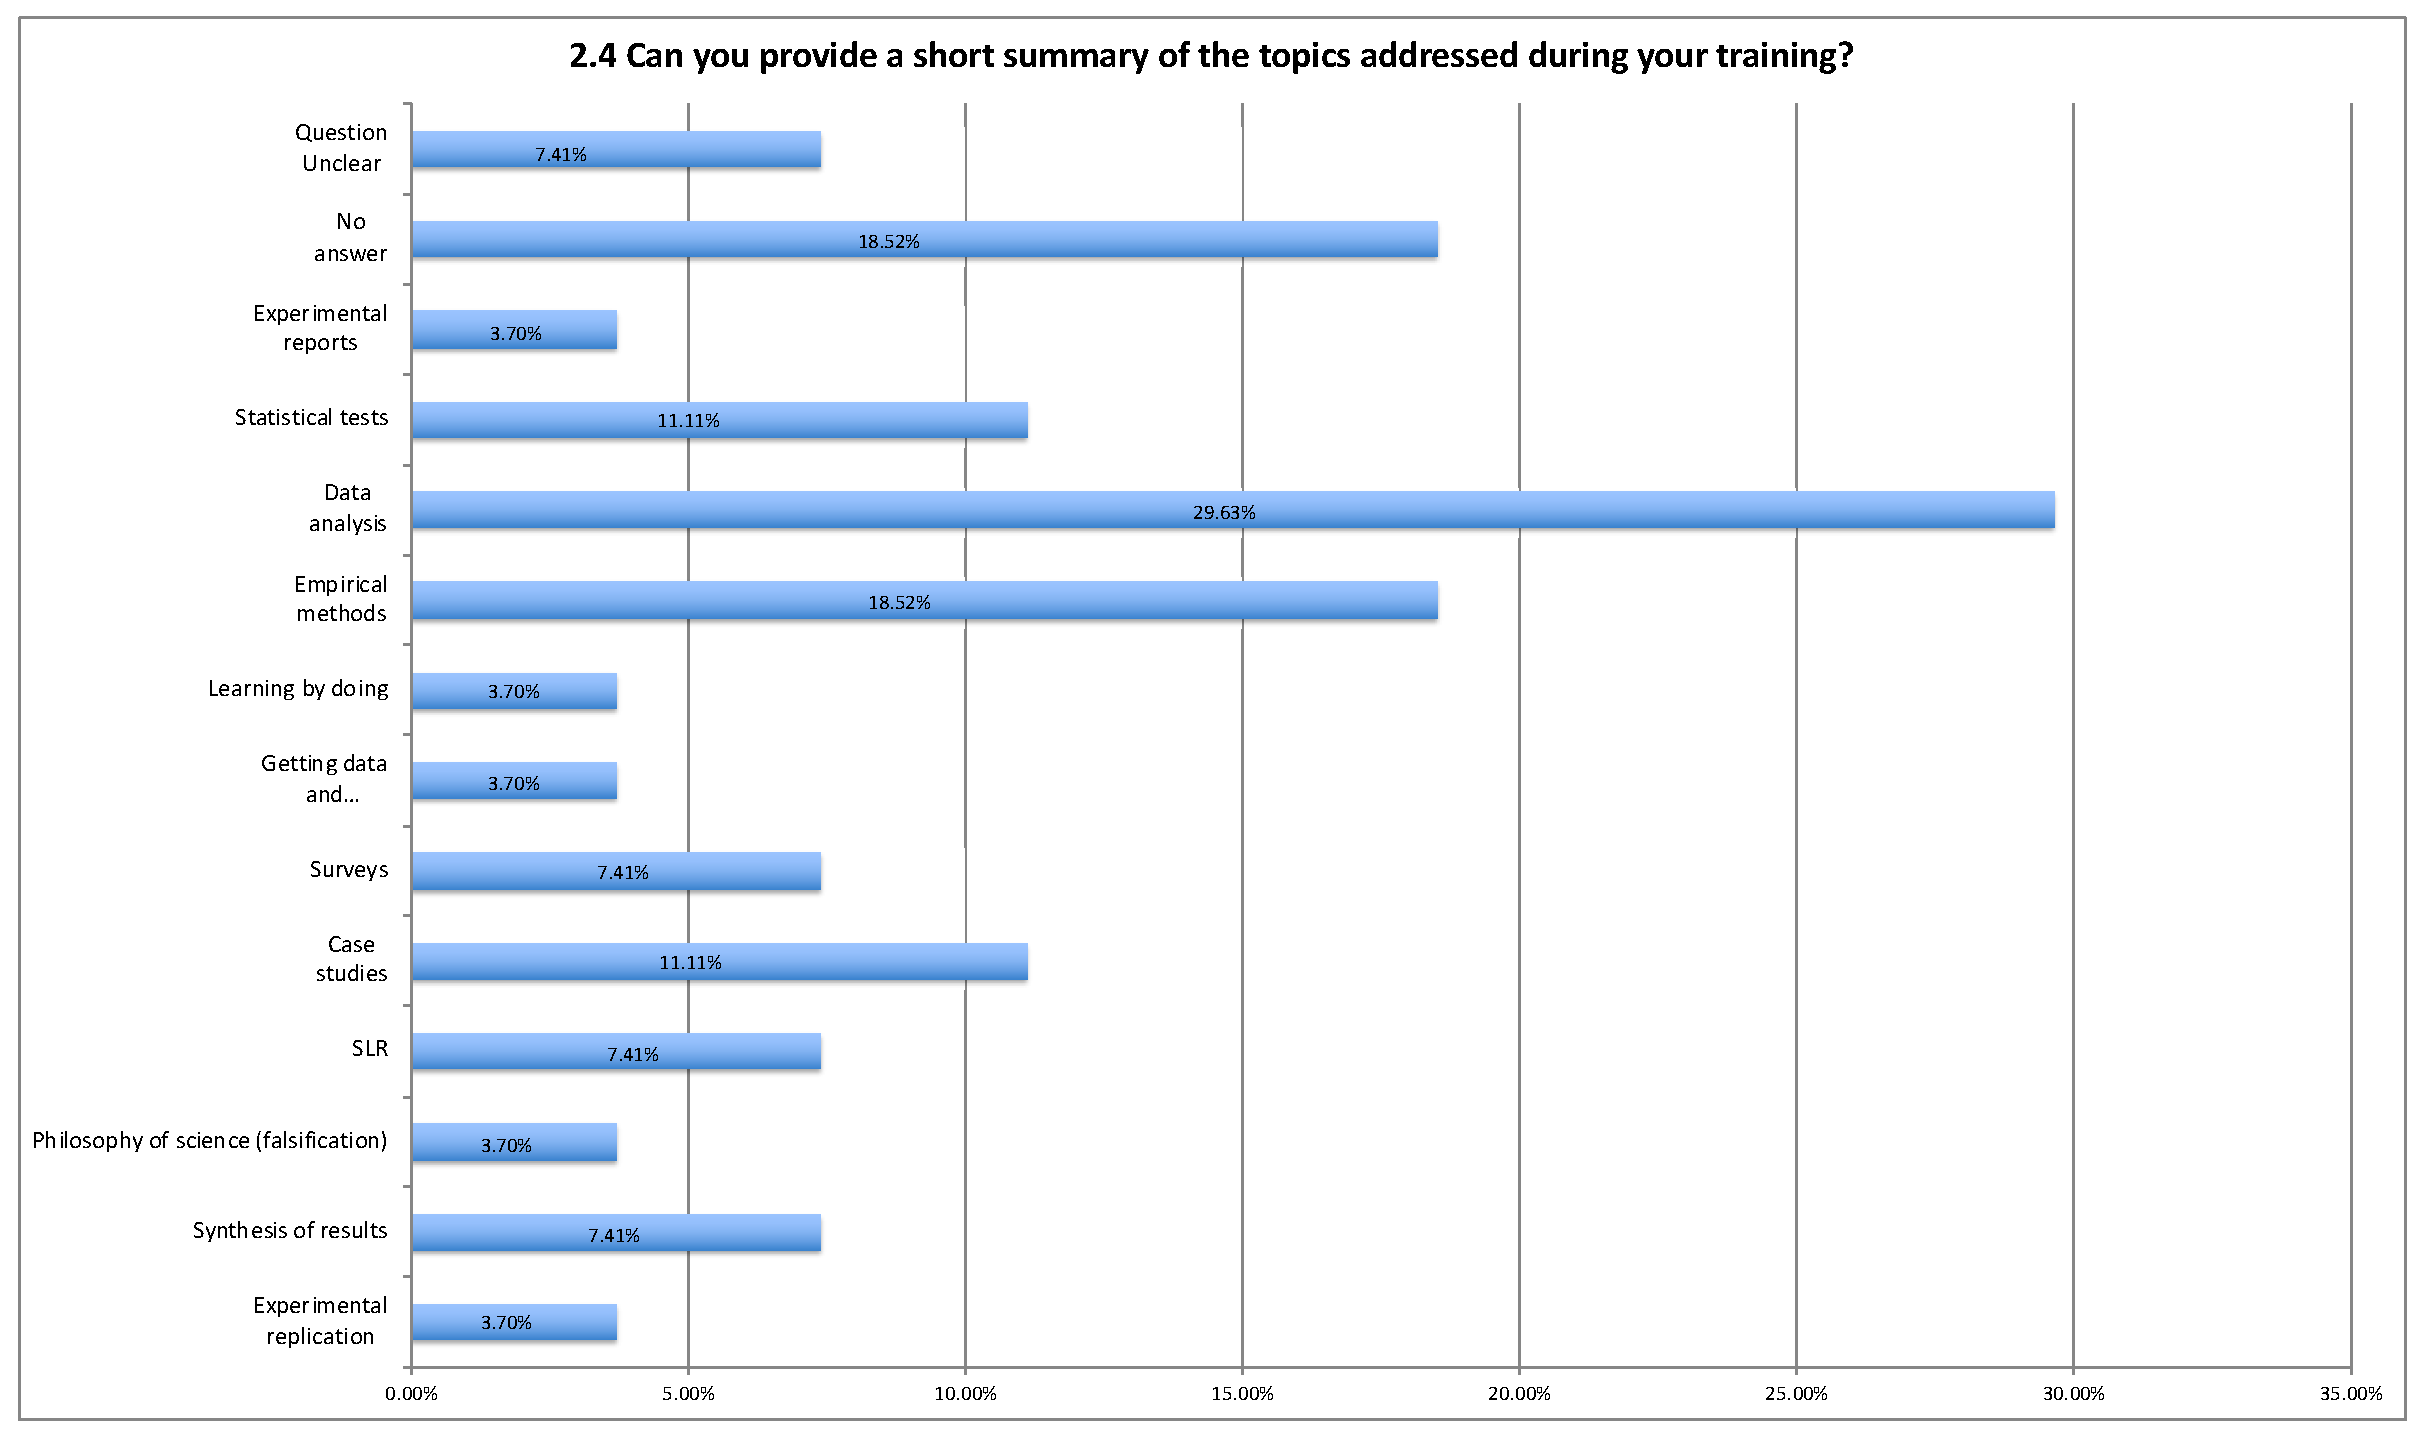
\includegraphics[width=18cm]{Images/Topics-SE-experimentation-training}
	\caption{Topics considered on SE experimentation training}
	\label{fig-topics-training}
\end{figure*}

\subsection{Training materials}
Por training materials, nos referimos a los libros, art�culos, etc., que han sido utilizadas por los investigadores para su formaci�n. La encuesta mostr� que las fuentes usadas son escasas, tal y como muestra la Fig. \ref{fig-resources-training}. Los encuestados indican que el libro de Wohlin et al. \cite{Wohlin2012-Experimentation} es el m�s popular entre los investigadores de SE (67\%), mientras que los libros de Juristo et al. \cite{Juristo-2001-SE-experimentation} y Runenson et al. \cite{Runenson-2012-SE-case-study} le siguen en popularidad en un 15\% de los casos.

\begin{figure*}[htbp!]
	\centering
	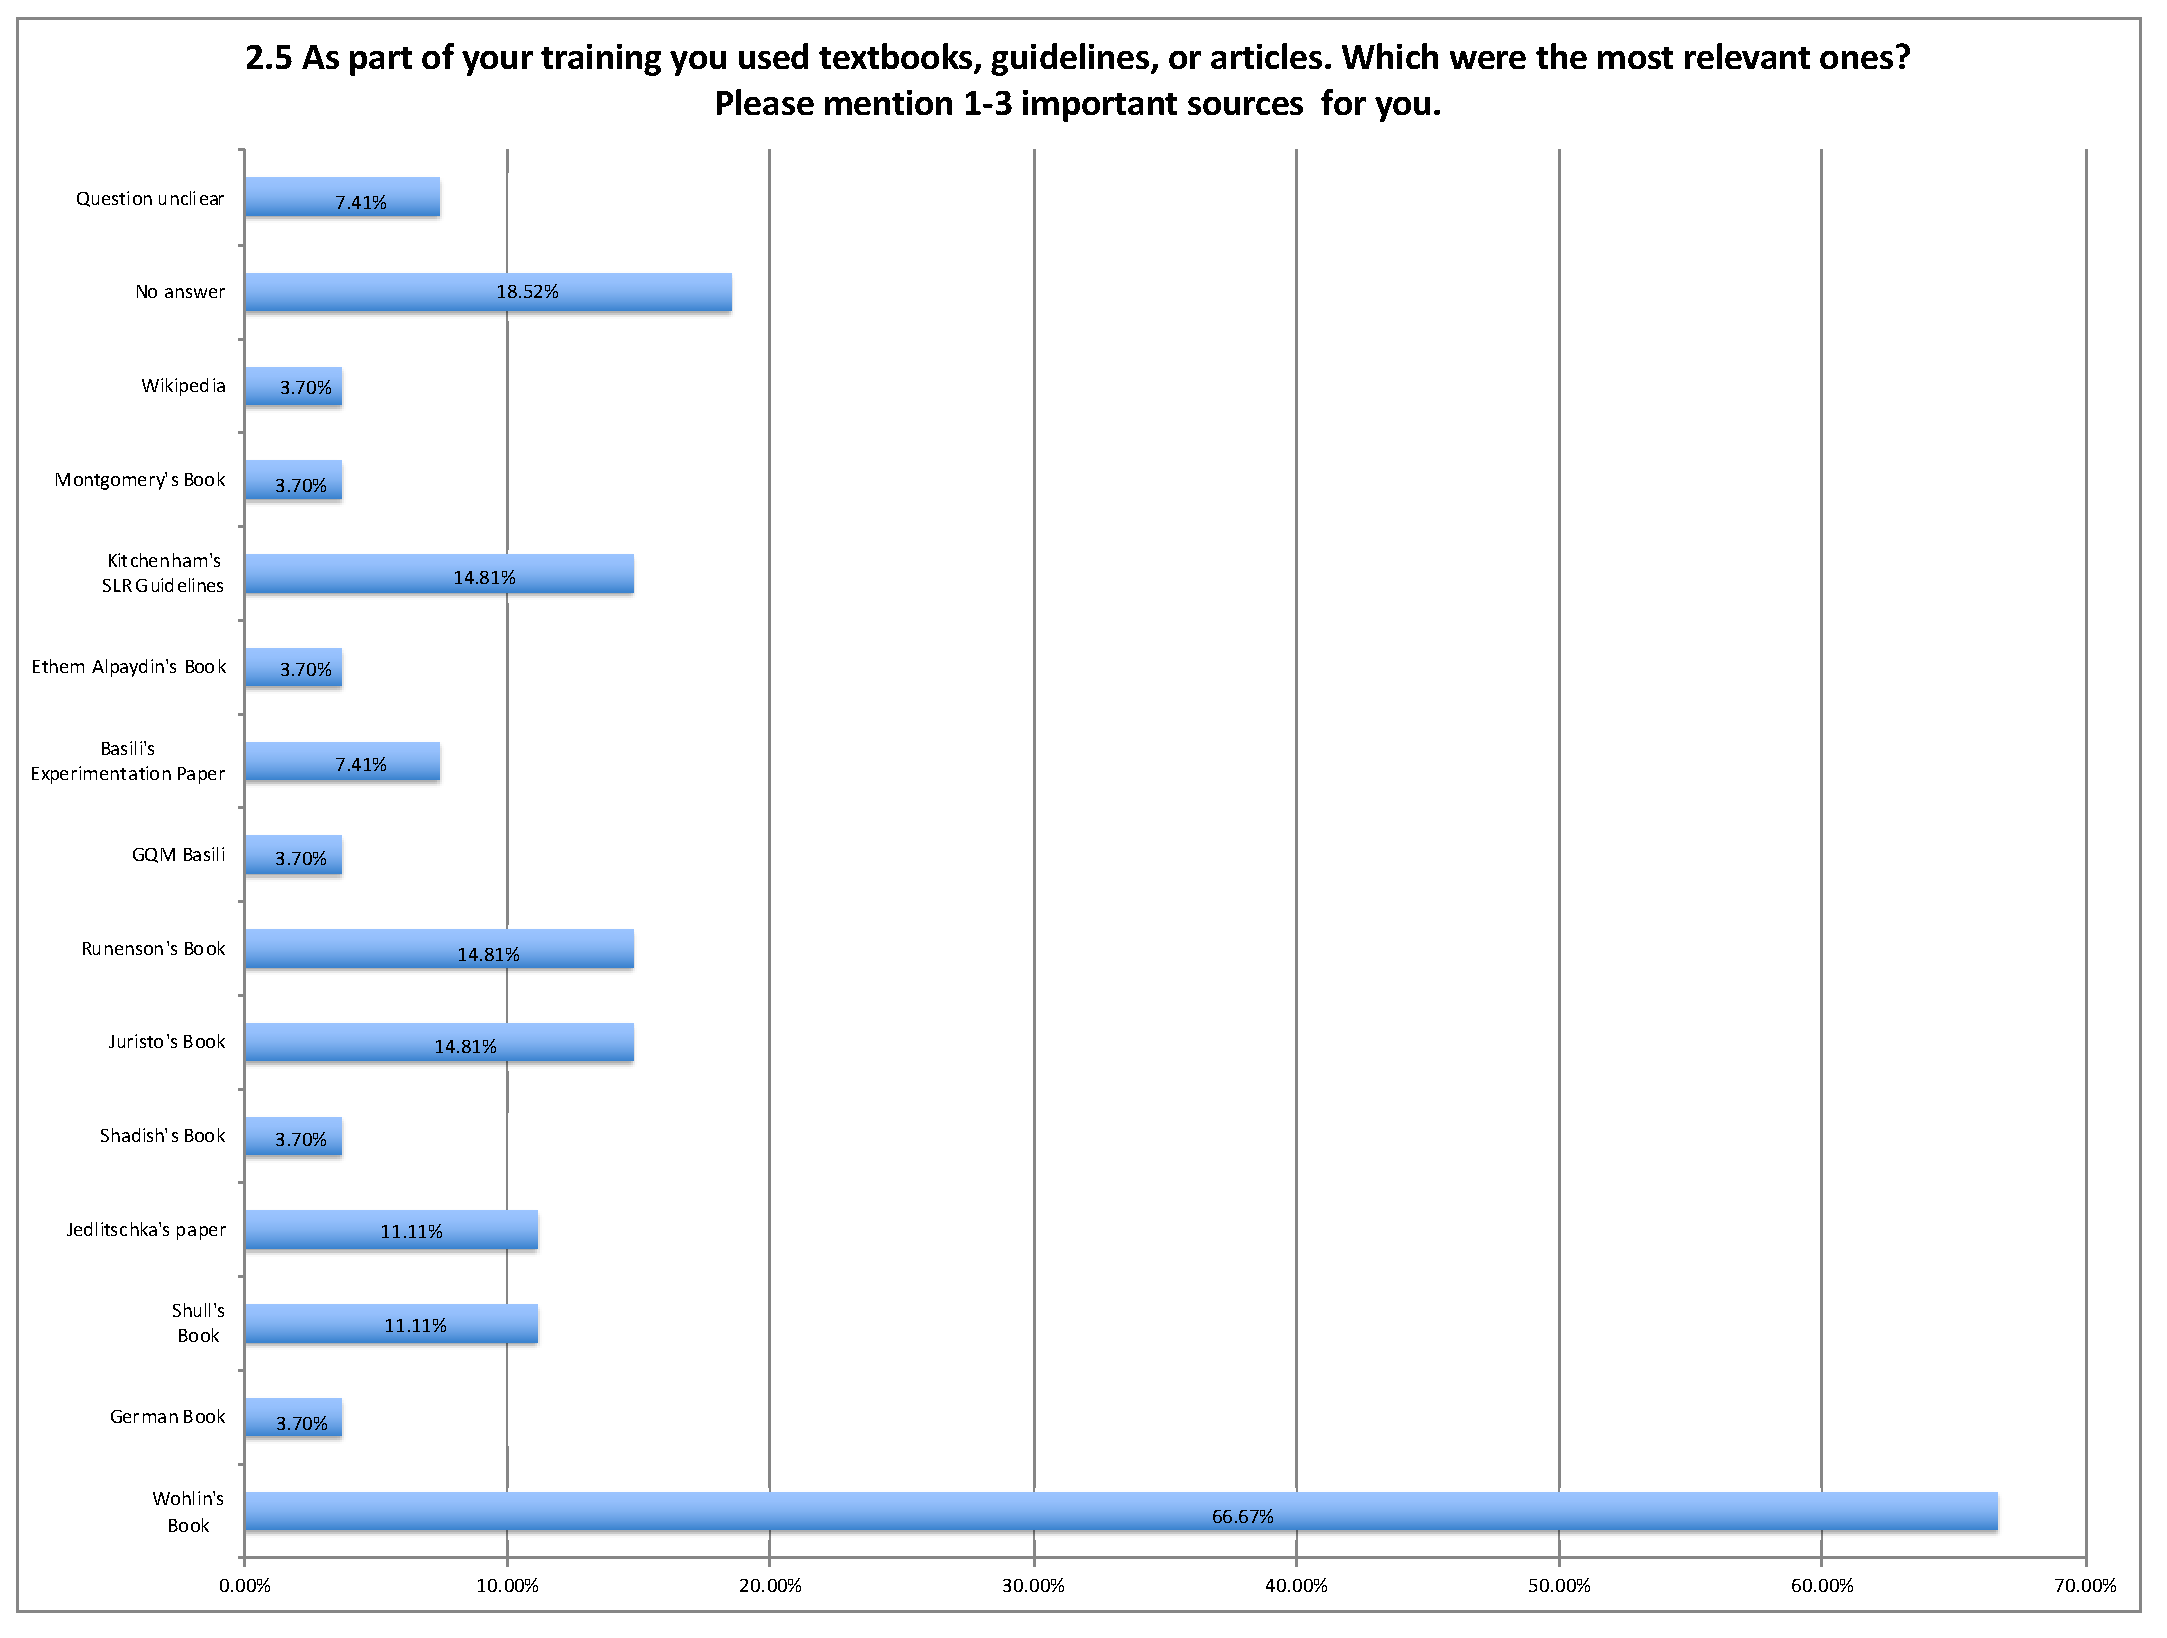
\includegraphics[width=17.5cm]{Images/Experimentation-training-resources}
	\caption{Base materials for learning SE experimentation}
	\label{fig-resources-training}
\end{figure*}

Es preciso indicar que un alto porcentaje de encuestados (29\%) no indica cuales fueron las fuentes utilizadas en su formaci�n en SE experimentation. Esto podr�a justificarse por la utilizaci�n de otras fuentes m�s ligadas a la pr�ctica, como los reportes experimentales o art�culos espec�ficos. A este respecto, hemos preguntado a los investigadores en qu� ha consistido su formaci�n pr�ctica. Casi un 60\% no respondi�, lo cual probablemente indica que la pregunta no estaba bien formulada. A�n as�, el 40\% de respuestas mostradas en la Figura \ref{fig-way-researchers-learn}, muestra que los investigadores aprendieron a experimentar en la pr�ctica principalmente leyendo reportes experimentales notables (25.93\%), tales como the Basili's experimentation paper \cite{Basili-1986-ESE} y the Jedlitschka's experimentation paper \cite{Jedlitschka-2005-GuideLines-ESE}, pidiendo recomendaciones de investigadores expertos en experimentaci�n (18.52\%) y leyendo libros de experimentaci�n de uso cotidiano en la comunidad (14.81\%), tales como The Wohlin's book \cite{Wohlin2012-Experimentation} y The Juristo's book \cite{Juristo-2001-SE-experimentation}. Este resultado est� en concordancia con el resultado SR2 de la etnograf�a de SE, donde se concluy� que las fuentes utilizadas para la formaci�n de los experimentadores en SE son m�ltiples.

\begin{figure*}[htbp!]
	\centering
	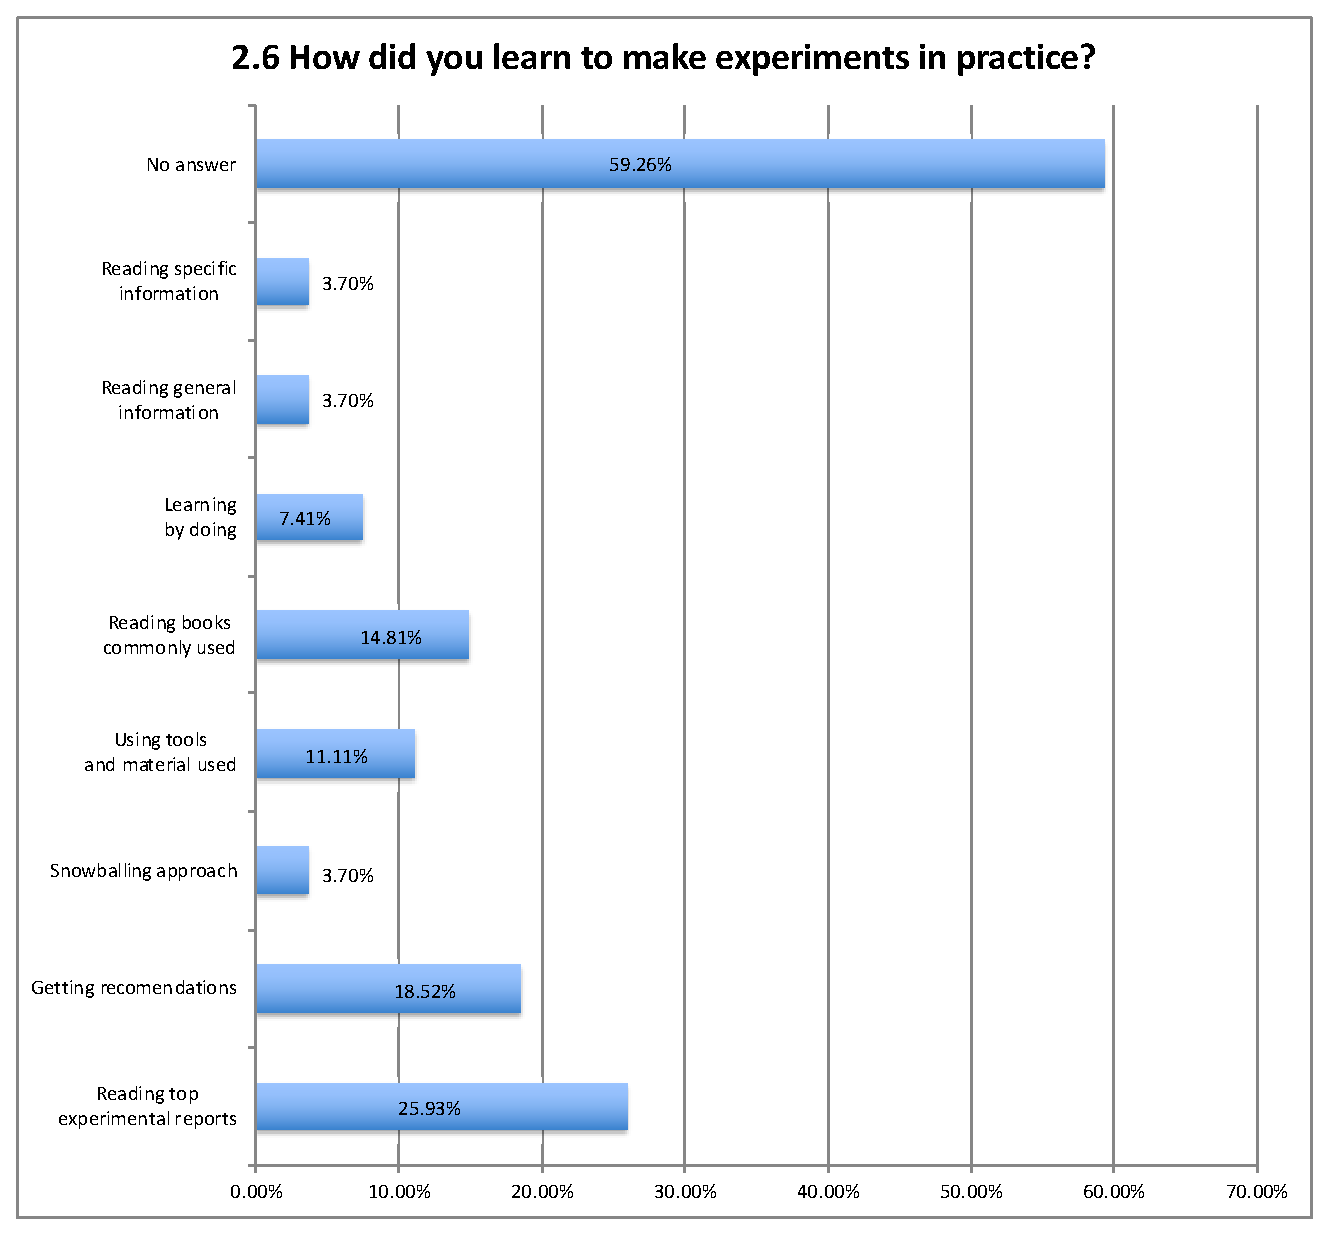
\includegraphics[width=10cm]{Images/Way-researchers-learn-SE-experimentation}
	\caption{The way in which researchers learn SE experimentation}
	\label{fig-way-researchers-learn}
\end{figure*}

\subsection{Terminological diversity}
Los hallazgos obtenidos en el estudio etnogr�fico (SR3) sugieren que la manera en que los investigadores adquirieron el conocimiento de experimentaci�n representa a una de las principales causas de la diversidad conceptual y operativa observada. La variedad en las fuentes y tipos de formaci�n en experimental SE sugieren que la diversidad terminol�gica deber�a aparecer tambi�n en la generalidad de investigadores de experimental SE.

A este respecto, la estrategia que hemos utilizado en el survey ha consistido en indagar sobre ciertos conceptos que consideramos b�sicos, y observar la interpretaci�n que los encuestados hac�an de los mismos. Por ejemplo, cuando se indag� sobre �Qu� palabra usa usted para referirse al proceso donde se definen los detalles del experimento y se eval�an las amenazas a la validez?, el 48\% de encuestados no respondi�, un 26\% cit� el t�rmino \textquotedblleft Planning\textquotedblright, un 18\% a \textquotedblleft Design\textquotedblright, un 4\% a \textquotedblleft Experiment setting\textquotedblright, y un 4\% a \textquotedblleft Guideline\textquotedblright. Solo en muy pocas preguntas de este estilo se not� consenso. Por ejemplo, cuando se pregunt� �Qu� palabra usa para referirse al proceso en el que se estudian los datos experimentales o las m�tricas, probablemente utilizando m�todos estad�sticos?, el 37\% cit� el t�rmino \textquotedblleft Data Analysis\textquotedblright.

Tambi�n fueron planteadas preguntas enfocadas en la conceptualizaci�n de la experimentaci�n. Por ejemplo, cuando se solicit� definir el concepto de: \textquotedblleft Selecci�n de sujetos\textquotedblright, casi un 70\% de los encuestado no respondi�, y del 30\% de respuestas obtenidas, ninguna coincid�a entre s�. Solo en muy pocos conceptos hubo cierto grado de consenso. Por ejemplo, cuando se pidi� a los investigadores encuestados que definieran el concepto: \textquotedblleft Hypothesis formulation\textquotedblright, un 22\% respondi� \textquotedblleft Define testable statistical hypothesis\textquotedblright~y un 11\% \textquotedblleft What to check through the experiment\textquotedblright, lo que representa un alto grado de coincidencia considerando que un 63\% no respondi�. El set de preguntas planteadas puso de manifiesto la existencia de una marcada diversidad conceptual en la comunidad de SE emp�rica.

\subsection{Operational diversity}
Los hallazgos en torno al estudio etnogr�fico muestran que el protocolo seguido en la experimentaci�n dentro de un grupo de investigaci�n en SE no es uniforme. En el survey se plantearon preguntas enfocadas en las actividades que realizan los investigadores de la comunidad de ESE al momento de llevar a cabo un experimento, con el prop�sito de contrastar el estudio etnogr�fico. La Fig. \ref{fig-Operational-Diversity-ESE-Community} muestra las actividades de experimentaci�n con las que se identifican los investigadores de la comunidad ESE. Las respuestas exhiben un alto nivel de coherencia, ya que al final hemos obtenido la descripci�n de procesos experimentales completos. Sin embargo, la diversidad operativa indicada en SR4 se manifiesta claramente debido a que, en lugar de 1 o 2 procesos, hemos obtenido la definici�n de 7 procesos distintos. Las mayores diferencias entre los procesos ocurren a nivel de las actividades de validity evaluation, data set reduction, results documentation y experiment report.

\begin{figure*}[htbp!]
	\centering
	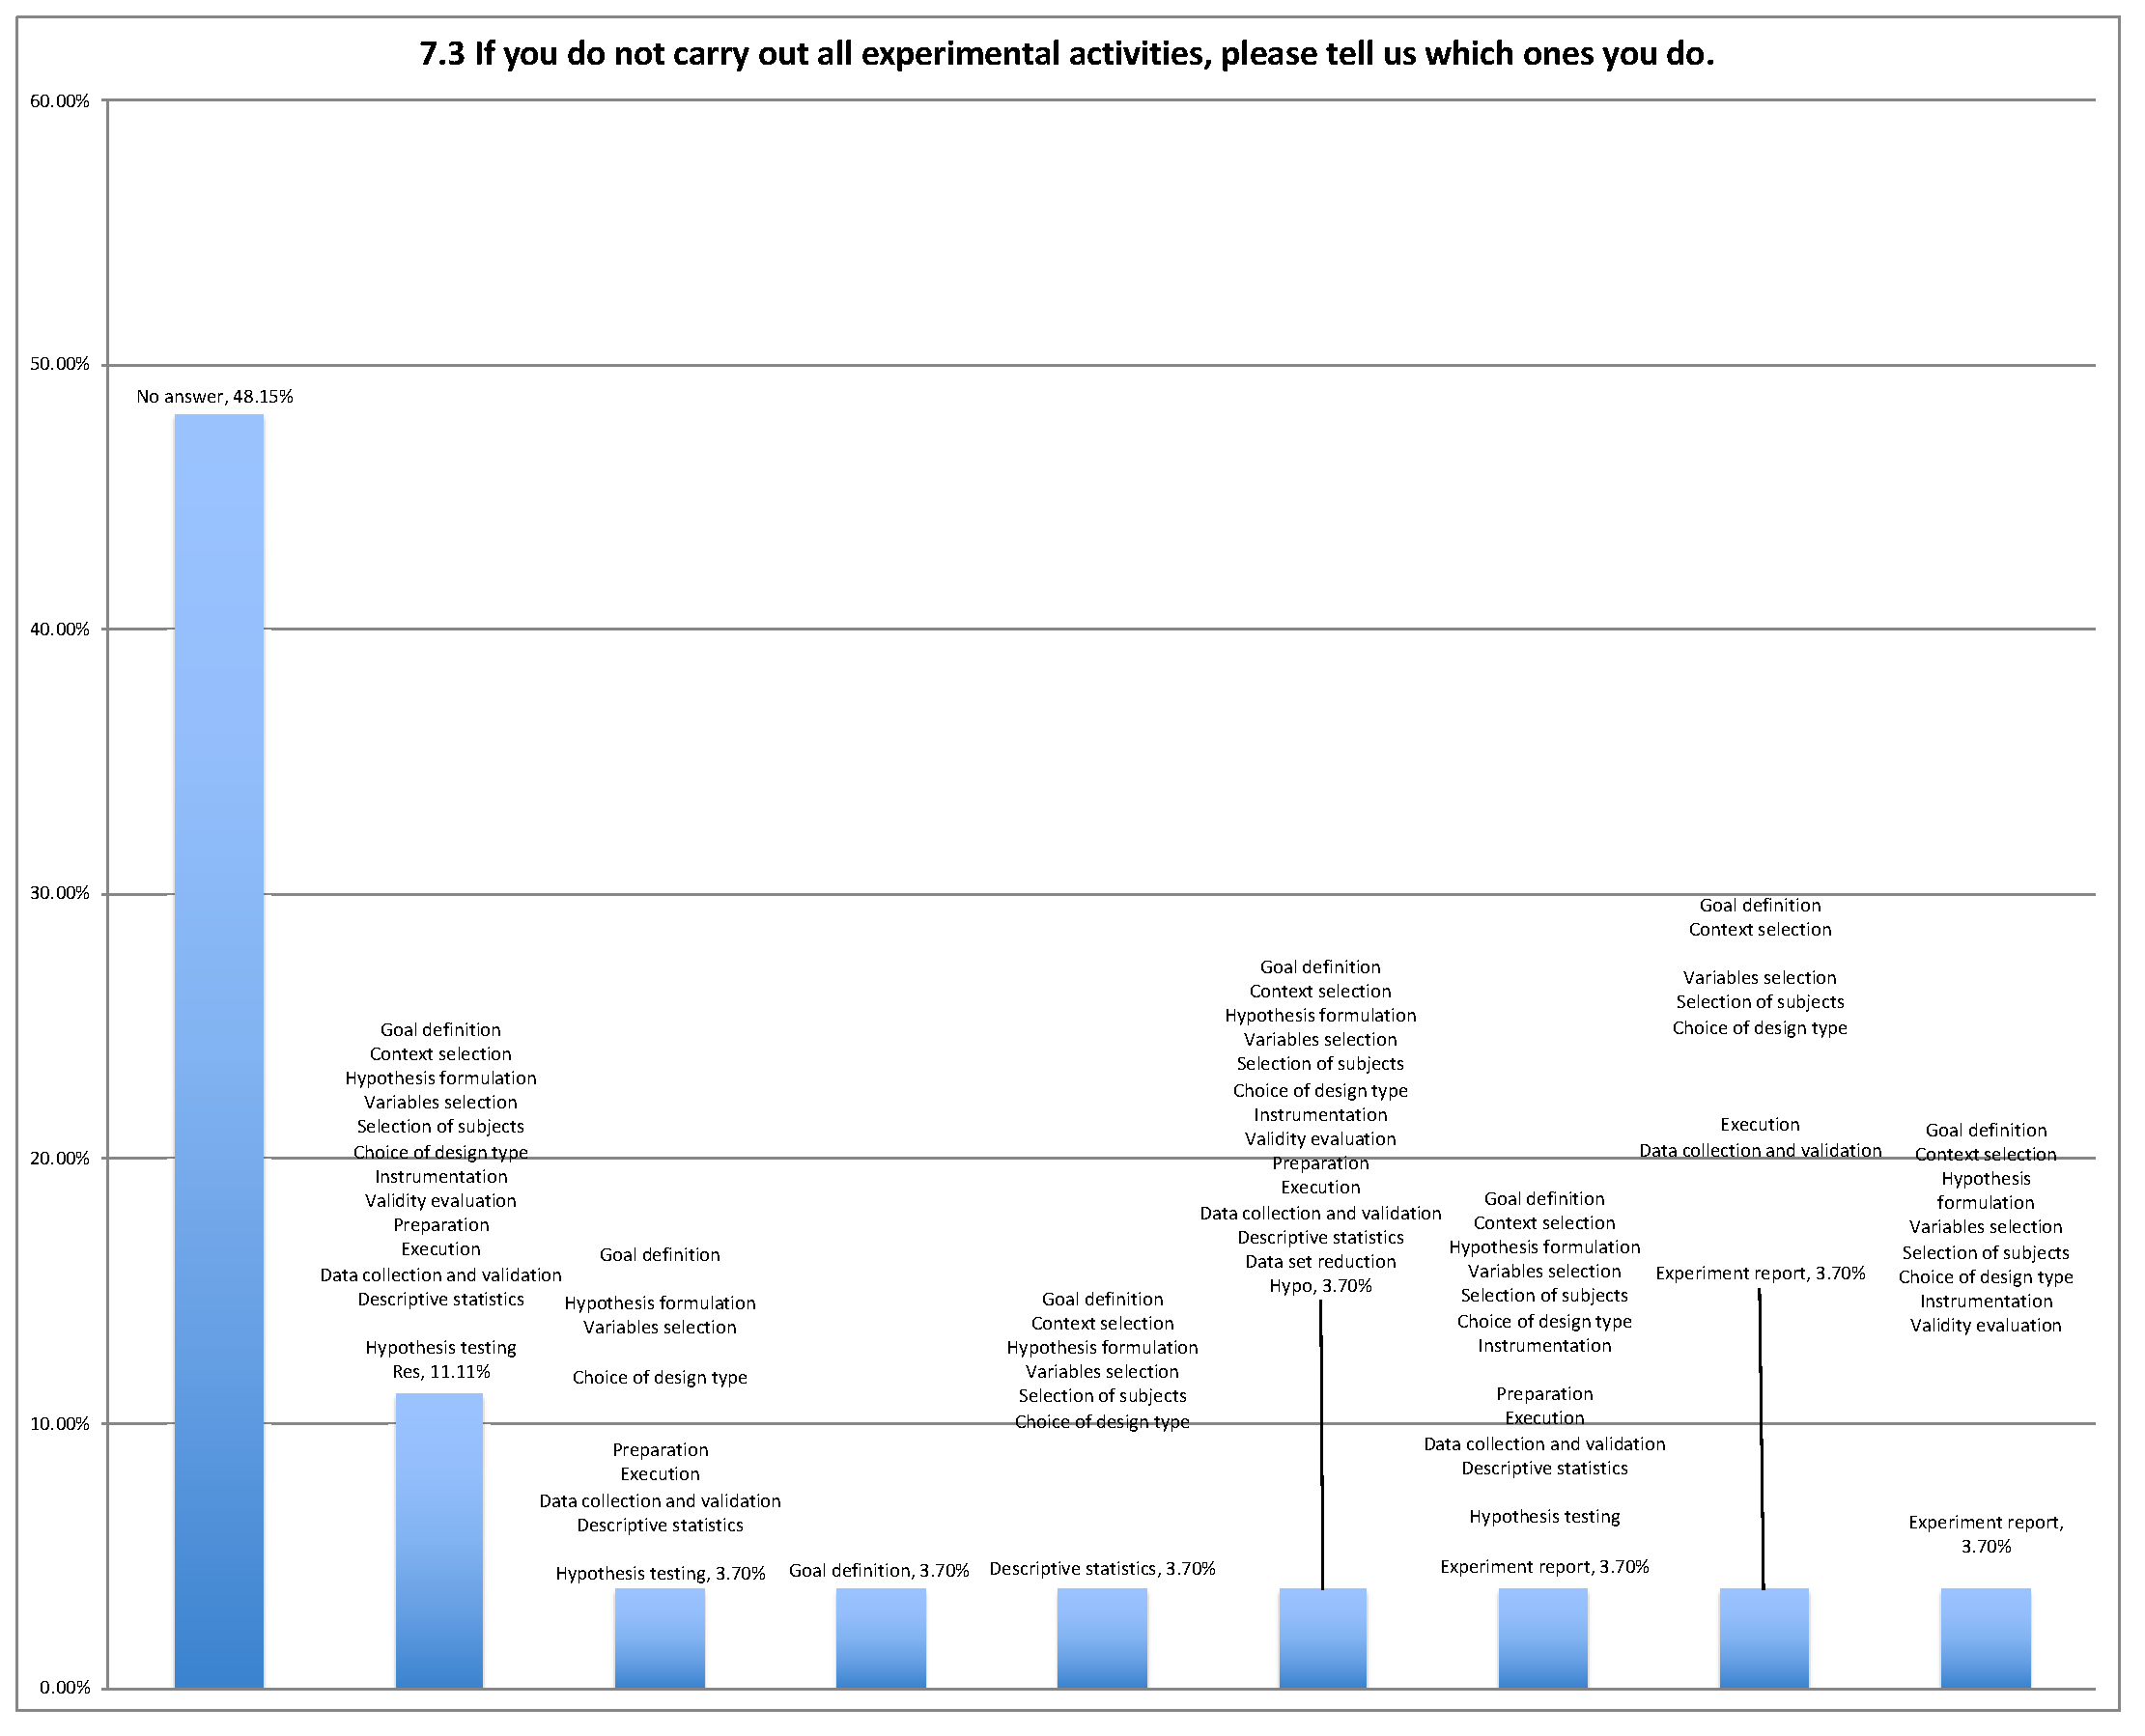
\includegraphics[width=17cm]{Images/Operational-Diversity-ESE-Community}
	\caption{Operational Diversity in Experimentation within the ESE Community}
	\label{fig-Operational-Diversity-ESE-Community}
\end{figure*}

\subsection{Roles}
Un aspecto bastante caracter�stico obtenido en la etnograf�a de SE es la existencia de roles (SR7). Aunque aproximadamente un 48.15\% de los encuestados no respondi� a la pregunta If you do not carry out all experimental activities, please tell us which ones you do?, un 37.04\% indican que no todas las actividades de experimentaci�n son llevadas a cabo por un solo investigador, lo cual es corroborado por un 33.33\% que indican que la complejidad del proceso de experimentaci�n define roles, e incluso un 29.63\% concuerda en que las actividades realizadas son distribuidas de acuerdo con las habilidades o conocimiento de los investigadores.



%Finalmente, encontramos que al parecer para los investigadores encuestados no es del todo claro el prop�sito de la SE experimentation. Aunque la mayor�a de investigadores encuestados (62.96\%) indican que la experimentaci�n esta orientada a la creaci�n de conocimiento en base a datos emp�ricos y a m�ltiples replicaciones para ser transferido a la industria y a la academia; no obstante, un 33.33\% no indican cual es el prop�sito de hacer experimentos en SE, de la mano de otro 25.93\% que tambi�n responde que los experimentos sirven para ganar conocimiento acerca de un fen�meno bajo estudio y para publicar eventualmente los resultados de experimentos aislados (ver Fig. \ref{Purpose-SE-Experiments}).

%\begin{figure*}[htbp!]
%	\centering
%	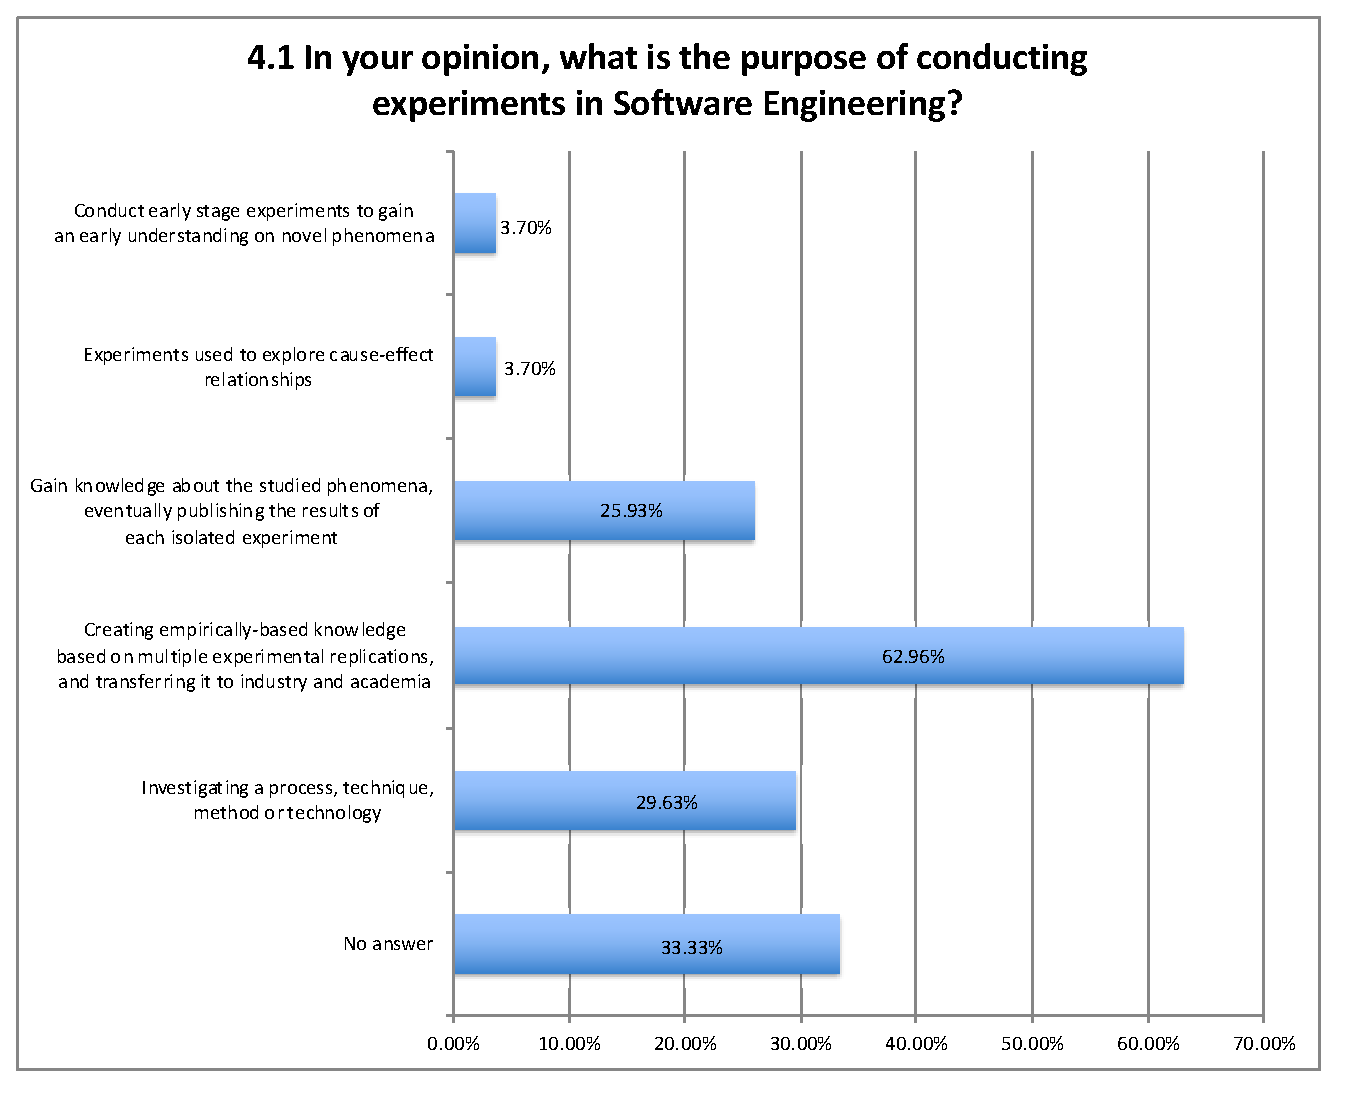
\includegraphics[width=12cm]{Images/Purpose-SE-Experiments}
%	\caption{Purpose of SE Experiments}
%	\label{fig-Purpose-SE-Experiments}
%\end{figure*}

%Esta situaci�n se corrobor� al indagar sobre las situaciones en las cuales un experimento es seleccionado como m�todo de investigaci�n (ver Fig. \ref{fig-why-experiments-done}), lo que no fue respondido por un 40.74\% de los encuestados. No obstante, quienes respondieron tuvieron criterios divididos: Un 18.52\% dijo que un experimento se realiza para aislar un fen�meno de inter�s o para confirmar un tipo espec�fico de hip�tesis; mientras que un 14.81\% indic� que se utiliza para comparar dos cosas o para investigar una relaci�n causa-efecto. Minoritariamente hubo investigadores que indicaron que un experimento se realiza dependiendo de la pregunta de investigaci�n planteada (11.11\%), como prueba de concepto (3.7\%) y cuando una replicaci�n es posible (3.7\%).

%\begin{figure*}[htbp!]
%	\centering
%	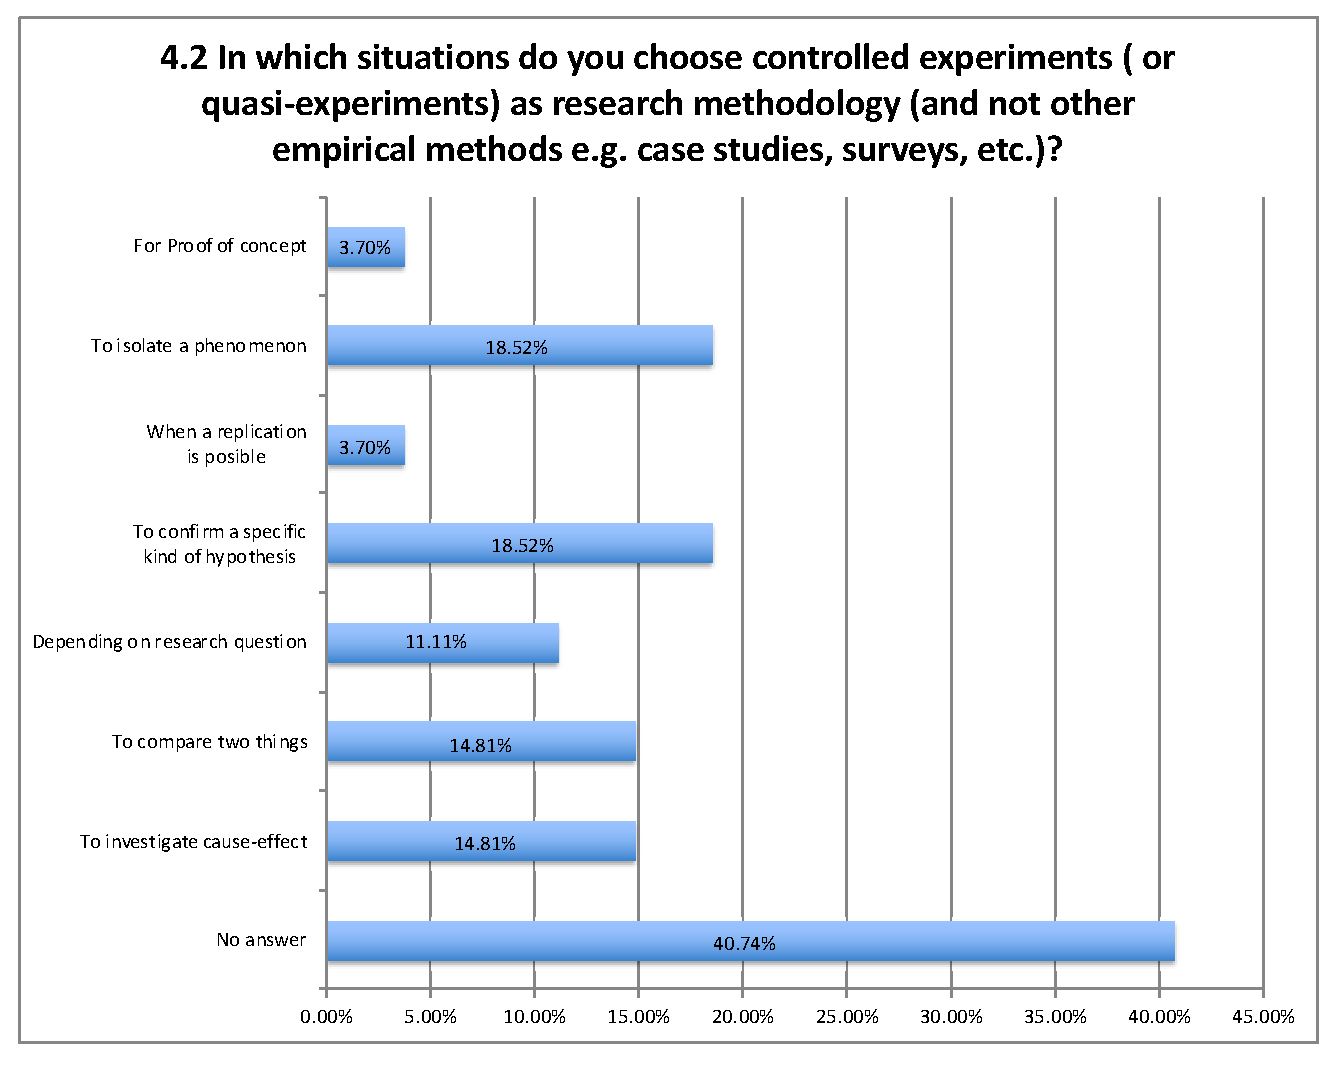
\includegraphics[width=12cm]{Images/Why-Experiment-Method-Selected}
%	\caption{Reasons why an Experiment is Selected as Research Method}
%	\label{fig-why-experiments-done}
% \end{figure*}

\subsection{Conclusiones}
Los resultados del survey han demostrado en gran medida que los hallazgos del estudio etnogr�fico que hemos realizado dentro de un grupo de investigaci�n en ESE son generalizables a la comunidad de ESE:

\begin{enumerate}[label={SrR\arabic*)}]
\item \textbf{Educaci�n:} La formaci�n en experimentaci�n de los investigadores en ESE ha sido informal: tiempos de entrenamiento variados, aprendizaje obtenido a partir de distintas fuentes y con contenidos muy variados. En la mayor�a de los casos, la formaci�n ha tenido una componente eminentemente pr�ctica.

\item \textbf{Fuentes:} Las fuentes de informaci�n utilizadas en la comunidad de ESE son generales y escasas.  El texto m�s popular en la comunidad es el libro de Wohlin et al \cite{Wohlin2000}, seguido de Juristo et al. \cite{Juristo-2001-SE-experimentation} y Runenson et al. \cite{Runenson-2012-SE-case-study}.

\item \textbf{Terminologia:} Los investigadores en ESE utilizan una terminolog�a muy variada para referirse a las fases del proceso experimental. 

\item \textbf{Operaci�n:} No existe un �nico proceso experimental, sino varios procesos compuestos de distintas etapas.
	
\item \textbf{Roles:} Los investigadores en ESE no son polivalentes. Asumen roles en el proceso experimental dependiendo de sus conocimientos y experiencia.
\end{enumerate}

\section{Experimentation in Biotechnology}\label{sec-bio-etnography}

El estudio etnogr�fico fue realizado en tres grupos de investigaci�n (\odnote{RODRIGO: nombre grupos?}) de Ingenier�a en Biotecnolog�a de la Universidad de las Fuerzas Armadas ESPE de Ecuador. \odnote{RODRIGO: Puedes poner un poco de historia y nombrar a sus lideres, tal y como has hecho al principio de la secci�n 4?.}

La selecci�n de estos grupos se ha producido por conveniencia. No obstante, no cabe duda de que el grupo de investigaci�n es altamente competitivo a nivel internacional, como se desprende de sus publicaciones, e.g., \cite{Vizuete-2016-green-Synthesis,Villarreal-2016-Effect-Arbuscular,Kumar-2016-In-Vitro-Evaluation}. Por consiguiente, creemos que los hallazgos del estudio etnogr�fico pueden ser extrapolables a la generalidad de grupos de investigaci�n en Biotecnolog�a. 

El estudio etnogr�fico no puedo ser exactamente igual al realizado con el GrISE porque est�bamos ''contaminados'' por la experimentaci�n en SE. Por este motivo, en lugar de realizar un proceso de acercamiento progresivo, decidimos abordar aquellas actividades que nos resultaron m�s fruct�feras en GrISE: a) Estudio de la literatura preferida de los grupos de investigaci�n, b) su material experimental y, particularmente, c) el conocimiento de los experimentadores. 

Dado que nos interesa especialmente comparar la experimentaci�n en SE y Biotecnolog�a, destacaremos las caracter�sticas diferenciales de Biotecnologia mediante subrayado, al igual que hemos realizado anteriormente en la Secci�n~\ref{sec-ESE-etnography}. En algunas ocasiones, una observaci�n realizada en Biotecnolog�a arroja luz sobre la experimentaci�n en SE. Por este motivo, pueden surgir a lo largo de la exposici�n caracter�sticas espec�ficas de SE (numeradas en azul), en paralelo con las caracter�sticas espec�ficas de Biotecnolog�a (marcadas en rojo). \odnote{RODRIGO: Creo que ser�a mejor poner S1, S2, B1, B2, etc.}

\iffalse

@book{Good2012,
	Author = {Good, Phillip I and Hardin, James W},
	Publisher = {John Wiley \& Sons},
	Title = {Common errors in statistics (and how to avoid them)},
	Year = {2012}}

@book{Huck2009,
	Author = {Huck, Schuyler W},
	Publisher = {Routledge},
	Title = {Statistical misconceptions},
	Year = {2009}}

@book{Vickers2010,
	Author = {Vickers, Andrew},
	Publisher = {Addison-Wesley Longman},
	Title = {What is a P-value anyway?: 34 stories to help you actually understand statistics},
	Year = {2010}}
	
@inproceedings{Reyes2018,
  author    = {Rolando P. Reyes and
               Oscar Dieste and
               Efra{\'{\i}}n R. Fonseca C. and
               Natalia Juristo},
  title     = {Statistical errors in software engineering experiments: a preliminary
               literature review},
  booktitle = {Proceedings of the 40th International Conference on Software Engineering,
               {ICSE} 2018, Gothenburg, Sweden, May 27 - June 03, 2018},
  pages     = {1195--1206},
  year      = {2018},
  doi       = {10.1145/3180155.3180161}
}
\fi

\subsection{First approximation}\label{subsec-first-approx-biok}

La investigaci�n comenz� a finales de 2014. Aunque los investigadores ya hab�amos adquirido experiencia en la experimentaci�n en SE, los primeros contactos fueron dif�ciles debido al n�mero de actividades de experimentaci�n que se realizan en Biotecnolog�a, as� como a la variedad de insumos e instrumentos que se precisan dependiendo del �rea de investigaci�n. Los experimentadores en Biotecnolog�a {\color{red}(?)} \ul{no realizaban un discurso general que probablemente podr�amos comprender, sino que utilizaban terminolog�a altamente espec�fica} perteneciente a cada �rea de investigaci�n.

Los grupos en cuesti�n manejan las �reas de conocimiento de: Biotecnolog�a Humana, Biotecnolog�a Ambiental y Biotecnolog�a Vegetal. {\color{red}(?)} \ul{La especializaci�n de la investigaci�n es muy marcada respecto a lo observado en SE}. En el GrISE, el mismo grupo se dedicaba a distintas investigaciones (testing, requisitos, TDD). En cambio, en Biotecnolog�a, las �reas de investigaci�n est�n mucho m�s compartimentalizadas.

Estos grupos est�n formados esencialmente por {\color{red}(?)} \ul{un l�der (que por lo general es un investigador director de un proyecto de investigaci�n o el jefe de un laboratorio), e investigadores que son estudiantes de doctorado y master}. \odnote{RODRIGO: No hay seniors? Por qu�?}

\subsubsection{Review of preferred literature}\label{subsubsec-study-literature-case-study-2}

Los experimentadores se�alaron como textos b�sicos de Biotecnolog�a experimental a distintos libros, e.g.: \textit{Biotechnology Fundamentals} by F.A.Khan \cite{Khan-2012-Biotechnology-Fundamentals}) y \odnote{RODRIGO: poner otro libro}. Tras su revisi�n, nos sorprendi� encontrar que, al igual que en la SE, {\color{red}(15)} \ul{el proceso de experimentaci�n en Biotecnolog�a est� descrito de forma general}. As� por ejemplo \odnote{RODRIGO: Alguna an�cdota??}

No obstante, adem�s de los libros indicados anteriormente, los experimentadores disponen de {\color{red}(7)} \ul{una amplia variedad de textos, gu�as, reportes, etc. espec�ficos por tem�ticas de investigaci�n}. Por ejemplo, la \textit{Biotecnolog�a Agr�cola} by de Solaiman et al. \cite{Solaiman-2014-Mycorrhizal} describe el uso de microorganismos que se aplican a cultivos para el uso sustentable del suelo; la \textit{Biotecnolog�a Vegetal} by Bahadur et al. \cite{Bahadur-2015-Plant-Biotechnology}, se estudian todas las �micas de \textit{Arabidopsis thaliana} como modelo para el mejoramiento gen�tico de otras plantas. Esto representa una diferencia sustancial con la SE, donde {\color{blue}(?)} \ul{no existen apenas (\mbox{\cite{}\url{https://doi.org/10.1002/stvr.1486}} podr�a ser una excepci�n) textos espec�ficos de experimentaci�n por sub-�reas}, e.g., testing o requisitos. \odnote{RODRIGO: Esto lo puedes colocar en la parte de SE de la tabla~\ref{tab:comparison}}.

\odnote{RODRIGO: Sirve este texto para algo??}
\begin{tcolorbox}

No obstante, el conocimiento adquirido sobre experimentaci�n en SE, el proceso generado para su abstracci�n (particularmente aquel proveniente de la revisi�n de textos no espec�ficos de SE) y el comentario un tanto contradictorio que hac�an tambi�n los miembros de los grupos de investigaci�n sobre que \textit{en el �rea de la Biotecnolog�a se estaban aplicando propuestas alternativas de dise�o de experimentos} (e.g.: dise�os basados en el enfoque \cite{Kumar-2014-design-experiment-bioprocessing}) \textit{para la formalizaci�n del proceso experimental}{\color{red}(14)}; nos impulsaron a la realizaci�n de este estudio.

\end{tcolorbox}

Las fuentes pertenecientes a cada sub-�rea {\color{red}(1)} \ul{utilizan una terminolog�a bastante uniforme, tanto a nivel de conceptos como de procesos}, e.g.,  el \textit{Handbook} by Walker et al. \cite{Walker-2008-Handbook-Biomethods} y el libro de Ausubel et al. \cite{Ausubel-2003-Molecular-Biology} exhiben grandes similaridades en los  protocolos experimentales utilizados para el estudio de �cidos nucleicos. Por el contrario, {\color{red}(2)} \ul{encontramos diversidad (terminol�gica y operativa) entre las fuentes de sub-�reas distintas}.

\odnote{Deber�amos poner un ejemplo, y aprovechar el ejemplo para afirmar que los textos en biotecnolog�a utilizan de forma natural sus propios conceptos en la descripci�n de los protocolos. En Software, existe una separaci�n entre la terminolog�a de la parte experimental y la terminolog�a de SE.}


\subsubsection{Review of experimental material}\label{subsubsec-study-materials-case-study-2}

El material experimental propio de los grupos est� formado por sus publicaciones, datos experimentales y las denominadas libretas de laboratorio. Las libretas de laboratorio son comunes en muchas disciplinas \cite{}\url{https://www.training.nih.gov/assets/Lab_Notebook_508_(new).pdf}, aunque no en SE. Consisten en \odnote{RODRIGO: Completar}. Todos estos materiales {\color{red}(12)} \ul{resultaron ser muy espec�ficos, en consonancia con la naturaleza propia de cada �rea de conocimiento}. Por ejemplo, \odnote{RODRIGO: Alguna an�cdota??}

Durante este segundo estudio etnogr�fico, no profundizamos en la terminolog�a y operativa espec�ficas de las sub-�rea de Biotecnolog�a a las que se dedicaban los experimentadores. No era de nuestro inter�s obtener un conocimiento granular sobre conceptos ajenos a SE, ya que dif�cilmente podr�an haber sido utilizados para una comparaci�n SE vs. Biotecnolog�a. Tal y como puede comprobarse en los modelos mostrados en las Figs.~\ref{fig-proceso-exp} y \ref{fig-conceptos-exp}, los conceptos y procesos recogidos en SE poseen un alto nivel de abstracci�n. En consecuencia, los modelos de experimentaci�n en Biotecnolog�a que preparamos durante la primera aproximaci�n (v�ase, por ejemplo, la Fig.~\ref{fig-concepts-initial-bio}) fueron igualmente de alto nivel. 

De todos modos, esto no debe hacernos olvidar que \odnote{hablar de nuevo de los conceptos propios de biotecnolog�a, a los que hac�a referencia en la nota anterior}.

\odnote{RODRIGO: Entiendo que las observaciones que aparecen abajo son los aspectos del proceso experimental de Bio que te llamaron la atenci�n. Es necesario que aparezcan en el modelo de la Fig.~\ref{fig-concepts-initial-bio}. Adem�s, deber�as destacar la diferencia con SE. Puedes incluso crear nuevos hallazgos en azul. Corrige tu el texto de abajo de forma coherente con el discurso que estamos haciendo. A mi me falta contexto para hacerlo bien.}

\begin{tcolorbox}

Nos llam� mucho la atenci�n que, a diferencia de la SE experimental, \textit{en Biotecnolog�a consideran como fase fundamental de su proceso experimental, la generaci�n de publicaciones{\color{red}(30)}}; paralelamente, \textit{gestionan de forma �gil la investigaci�n a nivel de documentaci�n y recursos utilizados; particularmente los recursos humanos, econ�micos y legales}{\color{red}(13)}.

Otra caracter�stica que nos pareci� peculiar de los grupos de investigaci�n estudiados, fue que \textit{los reportes experimentales son similares en formato y centran su discurso en los resultados generales de cada ensayo (experimento), los cuales se basan en la comparaci�n de tratamientos individuales}{\color{red}(29)}; as� mismo, \textit{encontramos indicios de que las actividades de experimentaci�n realizadas en Biotecnolog�a constituyen la estructura de los reportes experimentales que publican}{\color{red}(32)}.

Lo mismo ocurri� con los datos experimentales, dado que su preservaci�n no es muy importante en estos grupo de investigaci�n; de hecho, \textit{los datos obtenidos en las instancias experimentales son utilizados hasta su reporte, luego de lo cual son almacenados en repositorios experimentales locales o p�blicos para futuros re an�lisis o s�ntesis de resultados, o simplemente son descartado}{\color{red}(20)}. Estas caracter�sticas influyeron negativamente, sobredimensionando en un inicio nuestra percepci�n sobre la complejidad de la investigaci�n por realizar.
 
\end{tcolorbox}

\odnote{Hay una contradicci�n entre el ''desconocimiento'' afirmado aqu� y la ''falta de inter�s en obtener conocimiento granular'' indicado un poco m�s arriba.}

El desconocimiento por parte de los investigadores de las �reas de conocimiento de Biotecnolog�a limitaron los resultados de esta primera fase a la obtenci�n de un modelo gen�rico muy b�sico de la experimentaci�n en Biotecnolog�a. Para profundizar, aplicamos la misma estrategia que en SE y entrevistamos a los miembros de los grupos de investigaci�n objeto de estudio.
  
\subsection{Understanding The Biotechnology Experimental Process In Detail}\label{subse-experimental-process-biotech}

Nuestro prop�sito en este punto fue hacer expl�cito en detalle el conocimiento de experimentaci�n en Biotecnolog�a que tienen los miembros de los grupos de investigaci�n estudiados. En un inicio la actividad pareci� factible dado el inter�s en la investigaci�n, en adici�n a que los miembros de los grupos nos facilitaron reuniones con este fin. En efecto la actividad pudo desarrollarse sin mayores inconvenientes; sin embargo, la diversidad terminol�gica y operativa de la experimentaci�n entre �reas del conocimiento dificult� identificar un �nico proceso formal. Por lo tanto, nos vimos obligados a variar un tanto la t�cnica de abstracci�n del conocimiento en los acercamientos planificados con los miembros de los grupos.

\subsubsection{Interviews With Biotechnology Researchers}

El proceso de entrevistas en Biotecnolog�a se sustent� en el mismo cuestionario de preguntas abiertas y en la t�cnica de abstracci�n de conocimiento aplicados a los experimentadores de SE. Nuestra intenci�n inicial fue la misma de pormenorizar las actividades que cada experimentador lleva a cabo. Por cada sesi�n se gener� un reporte que fue validado por el experimentador en la sesi�n siguiente, hasta obtener un manuscrito que sintetiz� detalladamente las actividades experimentales que realizan.

Este acercamiento con los experimentadores de Biotecnolog�a, nos permiti� observar que \textit{la abstracci�n del proceso experimental en cada �rea de conocimiento sugiere que el protocolo experimental es formal y detallado}{\color{red}(17)}; de echo, \textit{cada experimentador lleva a cabo actividades definidas dentro del proceso de experimentaci�n, lo que no permite que exista solapamiento de actividades entre los experimentadores}{\color{red}(25)} y \textit{el conjunto de actividades realizadas por cada experimentador cumple un rol con una denominaci�n especifica}{\color{red}(26)}, por ejemplo el \textit{Biometrista se encarga del an�lisis de datos}{\color{red}(36)}.

La complejidad de abstraer de forma unificada un modelo �nico de los distintos enfoques experimentales de Biotecnolog�a estudiados a nivel de sus actividades, propici� realizar una s�ntesis de resultados por �rea y entre �reas de conocimiento, de las series de entrevistas realizadas, en miras de abstraer �nicamente actividades comunes y generales de la experimentaci�n en Biotecnolog�a.

Los esbozos realizados por algunos experimentadores en papel o en la pizarra (ver Figura \ref{fig-proc-exp-esbozo}) y el relato escrito abstra�do de las entrevistas sobre las actividades que realizan en el proceso experimental, permiti� ir sintetizando en un �nico modelo, que fue digitalizado utilizando software especializado. En cada sesi�n fue validado el modelo por los experimentadores, hasta obtener un modelo final (ver Figura \ref{fig-proceso-exp-final}).


\begin{figure}[htbp!]
	\centering
	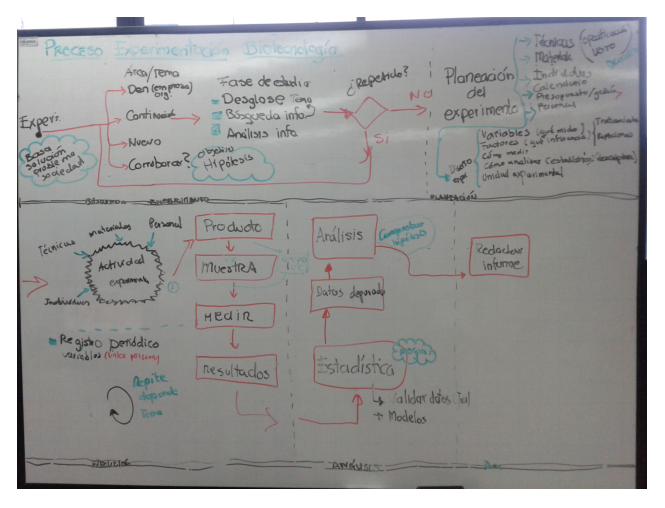
\includegraphics[width=3.2in]{Images/Outline-Process}
	\caption{Ejemplo de Esbozo de las Actividades Experimentales de Biotecnolog�a}
	\label{fig-proc-exp-esbozo}
\end{figure}

\begin{figure}[htbp!]
	\centering
	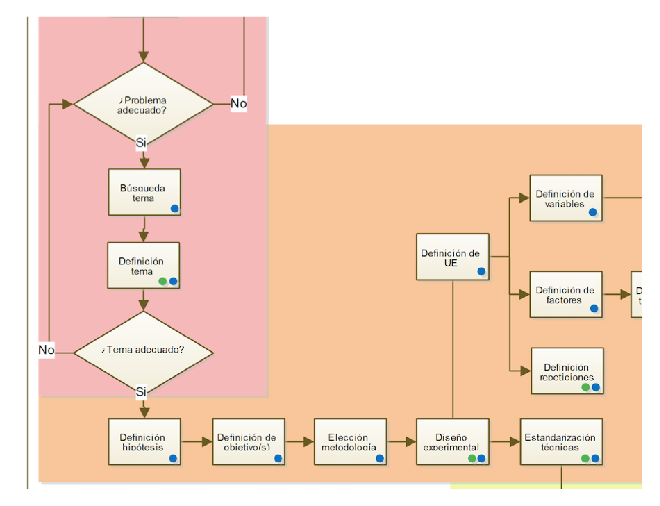
\includegraphics[width=3.2in]{Images/Final-Process}
	\caption{Extracto del Proceso Experimental de Biotecnolog�a}
	\label{fig-proceso-exp-final}
\end{figure}

La diversidad terminol�gica y operativa identificada entre las �reas de conocimiento estudiadas y nuestra intensi�n de obtener un modelo referente de la experimentaci�n realizada en Biotecnolog�a, nos condujo a la pretensi�n de homogeneizar en un solo modelo de procesos y conceptos la experimentaci�n en Biotecnolog�a. Para la parte conceptual, al igual que en SE experimental, propiciamos rondas de discusi�n entre los experimentadores de las distintas �reas de conocimiento estudiadas. 

\subsubsection{Harmonization Of Experimental Terminology In Biotechnology}

Las sesiones de discusi�n tuvieron como prop�sito armonizar la terminolog�a identificada en las �reas de conocimiento estudiadas. El proceso inici� con el debate sobre el modelo conceptual resultante de la review of preferred literature (ver Figura \ref{fig-concepts-initial-bio}). De cada sesi�n de discusi�n se obtuvo un producto intermedi�, el cual fue validado y depurado por el grupo en la siguiente instancia, hasta obtener un producto final (ver Figura \ref{fig-concepts-final-bio}).

\begin{figure}[htbp!]
	\centering
	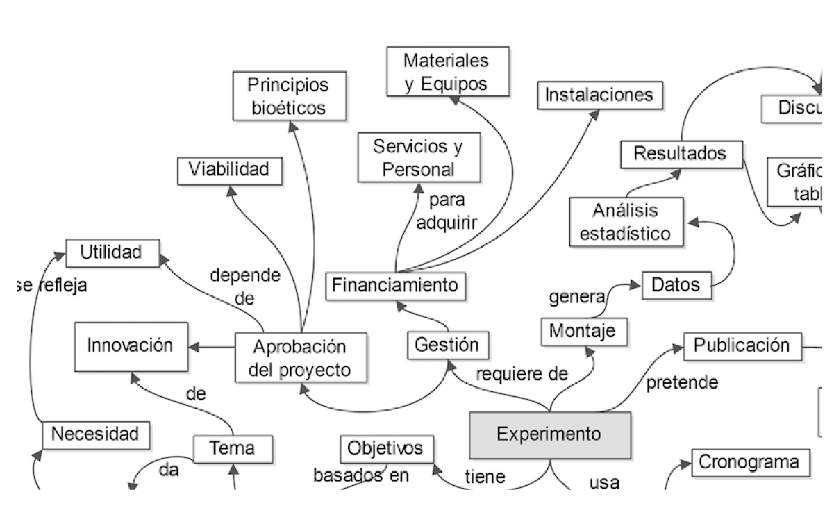
\includegraphics[width=3in]{Images/Concepts-Final-Bio}
	\caption{Extracto del Modelo Conceptual de Biotecnolog�a}
	\label{fig-concepts-final-bio}
\end{figure}

Las distintas sesiones de discusi�n nos mostraron que \textit{la cantidad de conceptos que intervienen en el proceso de experimentaci�n en Biotecnolog�a es alta}{\color{red}(18)}. Aunque no fue tan intenso el debate, las discusiones m�s importantes se centraron en los conceptos que difer�an de una a otra �rea de conocimiento, constat�ndose que \textit{los experimentadores de un mismo grupo de investigaci�n en Biotecnolog�a utilizan una terminolog�a com�n para comunicarse}{\color{red}(3)}; adicionalmente, se observ� que \textit{los conceptos manejados por los experimentadores en Biotecnolog�a corresponden a las actividades espec�ficas del rol que cumplen en cada proceso experimental}{\color{red}(27)}. La baja intensidad en las discusiones nos permiti� constatar que \textit{cada experimentador tiene una especialidad y por ende fue relativamente sencilla la conformaci�n del modelo conceptual}{\color{red}(28)}.

\subsection{Conclusions}

La revisi�n de la literatura preferente de los grupos de investigaci�n objeto de estudio nos permiti� observar que \textit{los textos gen�ricos de Biotecnolog�a no representan una gu�a efectiva para llevar a cabo experimentos en la pr�ctica en �reas espec�ficas de la Biotecnolog�a}{\color{red}(9)}. Sin embargo, \textit{la formalidad que se maneja en los reportes experimentales de estas �reas permite identificar f�cilmente las actividades llevadas a cabo en su proceso experimental}{\color{red}(33)}, \textit{lo que permiten replicar sin mayor complicaci�n los estudios realizados}{\color{red}(23)}; de hecho, \textit{tal es la claridad de los reportes que sin ser conocedores o expertos en el �rea, se puede entender claramente sus resultados, conclusiones y discusi�n}{\color{red}(21)}.

Otro de los factores que posiblemente ha incidido en la formalidad de los procesos experimentales estudiados, es \textit{el gran volumen de informaci�n que se maneja en estos grupos de investigaci�n, lo cual ha obligado a que el formato de los contenedores de datos experimentales sea est�ndar (hojas excel o repositorios)}{\color{red}(10)}, \textit{lo que facilita el acceso y utilizaci�n a otros grupos que investigan en la misma tem�tica}{\color{red}(11)}. De forma similar \textit{la formalidad operativa del proceso ha debido materializarse para mejorar la efectividad en la gesti�n e intercambio de la informaci�n{\color{red}(19)}}. Todo esto se ha visto reflejado en la \textit{construcci�n de mecanismos automatizados que guarden el v�nculo entre los experimentos y sus elementos (materiales, raw-data, dise�o, etc.) para ayudar a los experimentadores, entre otras cosas, a gestionar f�cilmente los datos experimentales}{\color{red}(22)}.

\section{Threats to Validity}\label{sec-threats}
%\odnote{RODRI: esta referencia es interesante para las amenzadas a la validez. S�lo vamos a citarla, porque no nos vamos a poner ahora a estudiar. Pero es interesante para el futuro.} $\rightarrow$ \url{https://www.researchgate.net/profile/Margaret_Lecompte/publication/255615696_Problems_of_Reliability_and_Validity_in_Ethnographic_Research/links/0f317538e4aae2a336000000/Problems-of-Reliability-and-Validity-in-Ethnographic-Research.pdf}
%\vspace{5mm}
Aunque existen algunos trabajos espec�ficos que abordan las amenazas a la validez de los estudios etnogr�ficos, e.g., LeCompte \& Goetz \cite{LeCompte-1982-Problems-Reliability-Validity-Ethnographic}, en este trabajo usamos como referencia a Runeson et al., \cite[p. 71 -- 73]{Runenson-2012-SE-case-study}, el cual a su vez se basa en el trabajo seminal de Yin \cite{Yin-2009-case-study}. En ambos trabajos, las amenazas a la validez se clasifican en cuatro tipos: (1) Validez de constructo, (2) validez interna, (3) validez externa y, (4) confiabilidad. En los siguientes apartados definimos cada uno de estos tipos de validez, y describimos las medidas preventivas adoptadas para sustentar la validez.

\subsection{Validez de constructo}
La validez de constructo se refiere al grado de concordancia entre la percepci�n que tiene el investigador y lo que realmente se investiga respecto al objeto estudiado, en funci�n de las preguntas de investigaci�n. Por ejemplo, si un constructo discutido en las preguntas de una entrevista no es interpretado en la misma manera por el investigador y por las personas entrevistadas, entonces existe una amenaza a la validez del constructo.

El m�todo etnogr�fico es totalmente opuesto a este tipo de amenaza a la validez, dado que la adquisici�n del conocimiento avanza a un ritmo lento, pero siempre en un contexto de consenso. Adicionalmente, en todo momento se utiliz� la t�cnica de triangulaci�n, que se fundamenta en considerar varios enfoques del objeto estudiado, para estructurar una perspectiva m�s amplia. Todo esto, de la mano de la utilizaci�n de varias t�cnicas para la elaboraci�n de constructos, por ejemplo: lectura, observaci�n, entrevistas, grupos de discusi�n, entre otros. Los diferentes enfoques incrementaron la posibilidad de identificar o resolver malentendidos entre los investigadores del RGUS.

Por otra parte, tambi�n prevenimos las amenazas de constructo, utilizando fuentes de informaci�n fiables, como por ejemplo, literatura est�ndar, material experimental del RGUS, el conocimiento de los experimentadores y la validaci�n cruzada del cuestionario del survey.

Finalmente, mencionar que, los constructos fueron validados iterativamente por los experimentadores e investigadores durante la vida �til del proyecto de investigaci�n.

\subsection{Validez Interna}
Existen numerosas amenazas a la validez internas relacionadas principalmente con efectos espurios, de las cuales Yin \cite{Yin-2009-case-study} relaciona solamente dos de ellas con los estudios cualitativos. La primera amenaza aborda la credibilidad de las relaciones causales encontradas durante la investigaci�n. Cuando el investigador afirma que existe una relaci�n causal ignorando posibles variables mediadoras y moderadoras, lo cual genera una amenaza a la validez interna. Afortunadamente, esta l�gica no es aplicable a estudios descriptivos o exploratorios como los surveys y las etnograf�as, dado que no se persigue la causalidad sino, como mucho, hallar correlaciones entre fen�menos.

\vspace{5mm}

\odnote{Para Oscar: Recordemos hablar de las correlaciones vs. causalidades en las conclusiones. Dicho de otro modo: nuestros hallazgos deber�an ser referendados por otros estudios.} 

\vspace{5mm}

La segunda amenaza interna es una extensi�n de la primera, a nivel de las inferencias. Realizar un estudio cualitativo como una etnograf�a implica realizar inferencias, tanto inductivas como abductivas, que incluyen fen�menos que no pueden ser observados directamente. Esta amenaza a la validez podr�a ser especialmente aplicable a esta investigaci�n. Par el caso de esta investigaci�n, los investigadores tuvieron contacto directo te�rico y pr�ctico con el fen�meno bajo estudio, de la mano de la gu�a y validaci�n de los experimentadores.

\subsection{Validez Externa}

La validez externa representa el grado de certeza acerca de la generalizaci�n de los hallazgos obtenidos en una investigaci�n. Esta amenaza es muy prominente para este estudio, ya que una de sus particularidades es que se realiz� en dos instancias (dos grupos de investigaci�n) de la poblaci�n bajo estudio (como poco, la totalidad de los grupos de investigaci�n en IS que aplican m�todos emp�ricos). Para asegurar la validez externa, hemos elegido grupos de investigaci�n muy representativos de las poblaciones bajo estudio. El survey, por su parte, permiti� contrastar los hallazgos del estudio etnogr�fico en IS con lo que se hace en la comunidad de IS experimental.

\subsection{Confiabilidad}

La confiabilidad de un estudio se refiere a la facilidad con la que las actividades de investigaci�n, e.g., el procedimiento de recolecci�n de datos, y los resultados obtenidos, e.g., la existencia de roles, pueden ser reproducidos por otros estudios que apliquen la misma metodolog�a en la misma muestra (o, m�s probablemente, en grupos de investigaci�n similares).

Para garantizar la confiabilidad de esta investigaci�n, hemos seguido fielmente la metodolog�a de investigaci�n indicada en la Secci�n~\ref{sec-metodologia}. Hemos almacenado todos los resultados intermedios y finales, los cuales est�n disposibles bajo demanda.

\section{Discussion and Conclusions}\label{sec-discussion-conclusions}
\subsection{Issues surrounding SE experimentation}
El estudio etnogr�fico devel� varias situaciones problem�ticas en torno a la experimentaci�n en SE, particularmente en lo referente a la comunicaci�n debida a la diversidad terminol�gica y operativa existente en el grupo de investigaci�n estudiado. El survey abord� m�s expl�citamente la problem�tica en torno a la experimentaci�n en la comunicad de ESE. Encontramos que m�s de un 60\% de los investigadores encuestados consideran que la experimentaci�n en SE es compleja debido a distintos factores (ver Fig. \ref{fig-Factors-Influencing-Complexity-ESE}). Por ejemplo, un 33.33\% considera que la complejidad de la experimentaci�n se debe a que el {\color{green}(SC9)} \ul{low sample size results in weak arguments which avoid addressing the industrial problems}; mientras que un 11\% cree que {\color{green}(SC10)} \ul{the abundant range of statistical tests options and poor knowledge about it results in an erroneous statistical study}.

\begin{figure*}[htbp!]
	\centering
	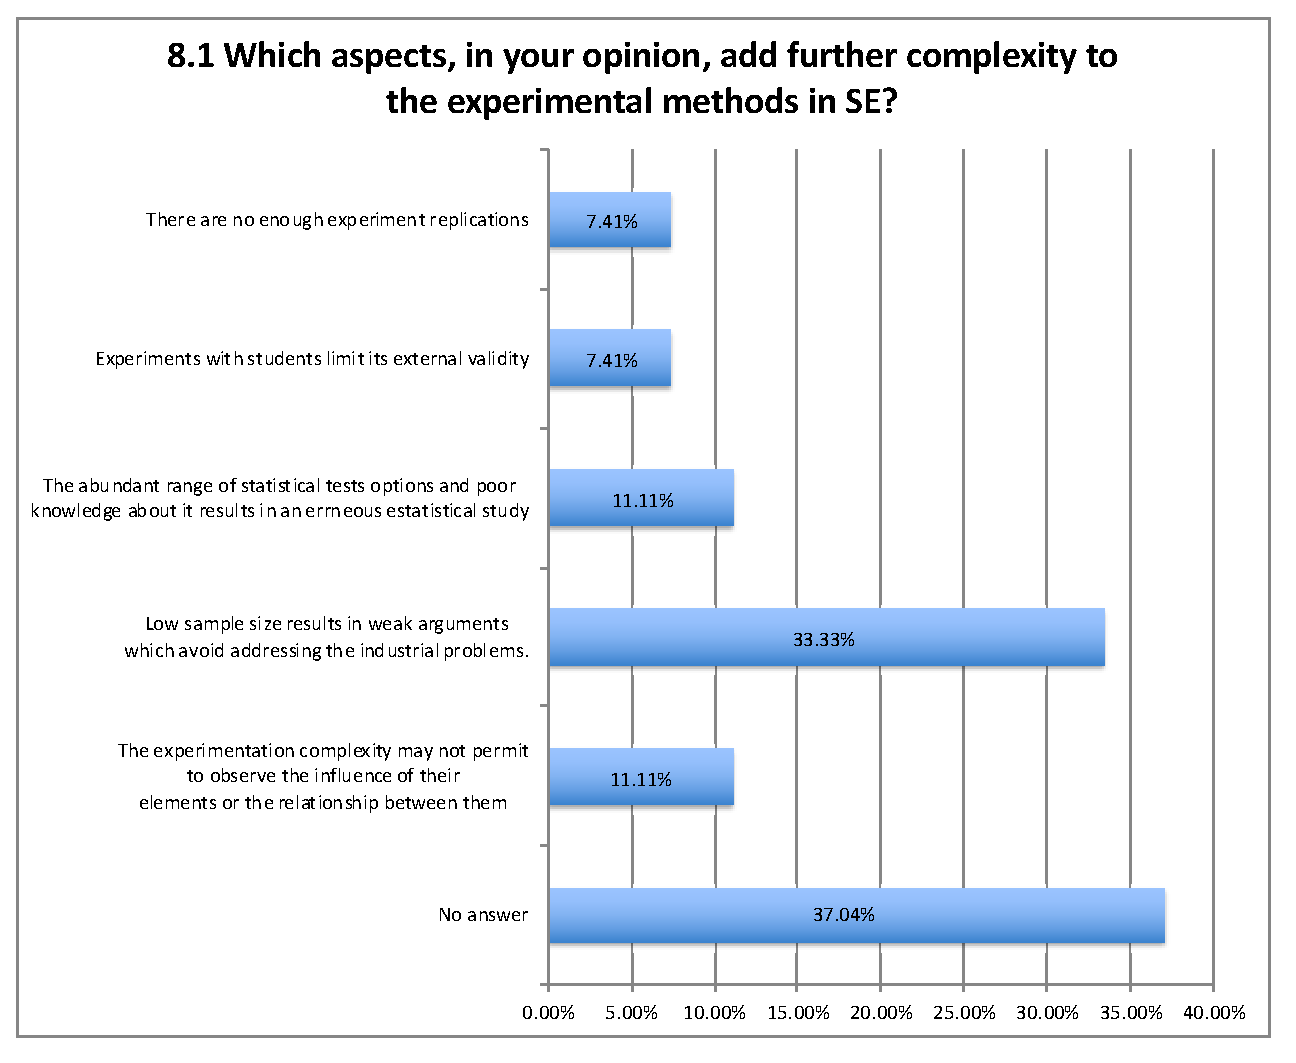
\includegraphics[width=12cm]{Images/Factors-Influencing-Complexity-ESE}
	\caption{Factors influencing the complexity of experimentation in SE}
	\label{fig-Factors-Influencing-Complexity-ESE}
\end{figure*}

As� mismo, un 11\% de los investigadores piensan que {\color{green}(SC11)} \ul{the experimentation complexity may not permit to observe the influence of their elements or the relationship between them}; mientras que otros investigadores son m�s espec�ficos y le atribuyen la complejidad de la experimentaci�n a que {\color{green}(SC12)} \ul{there are no enough experiment replications} (7.41\%) y a que los {\color{green}(SC13)} \ul{experiments with students limit its external validity} (7.41\%).

Por otra parte, otro problema remarcado en este estudio es el referido a la dificultad en la gesti�n de los datos. Un 14.81\% considera que {\color{green}(SC14)} \ul{el manejo y el an�lisis de los datos experimentales son complejos, lo que podr�a deberse en parte a las distintas maneras que tienen los investigadores para gestionarlos}: Un 66.67\% afirma que utilizan hojas de calculo, un 25\% repositorios de datos relacionales y un 44\% formatos propietarios. Por otra parte, un 7.41\% de los encuestados hace �nfasis en la limitada compartici�n de datos que existe, lo que es corroborado por mas de un 10\% de investigadores que consideran que {\color{green}(SC15)} \ul{la agregaci�n de datos entre replicaciones es compleja, quiz� en parte porque no existe un soporte adecuado para las replicaciones y la existencia del conocimiento t�cito}.

\begin{tcolorbox}

los aspectos que consideramos como problem�ticos en torno a la SE experimentation fueron corroborados en gran medida por los encuestados, e incluso se obtuvieron importantes recomendaciones a ser consideradas (ver Fig. \ref{fig-recommendations-improve-SE-experimentation}):

\begin{itemize}
  \item To have a common empirical source of knowledge
  \item To use simple guidelines to report findings
  \item To formalize the process
  \item To formalize the terminology
  \item To apply statistical test depending on experiment design
  \item To have a set of selected experimental subjects
  \item To receive quality formal courses
\end{itemize}

\end{tcolorbox}

\begin{figure*}[htbp!]
	\centering
	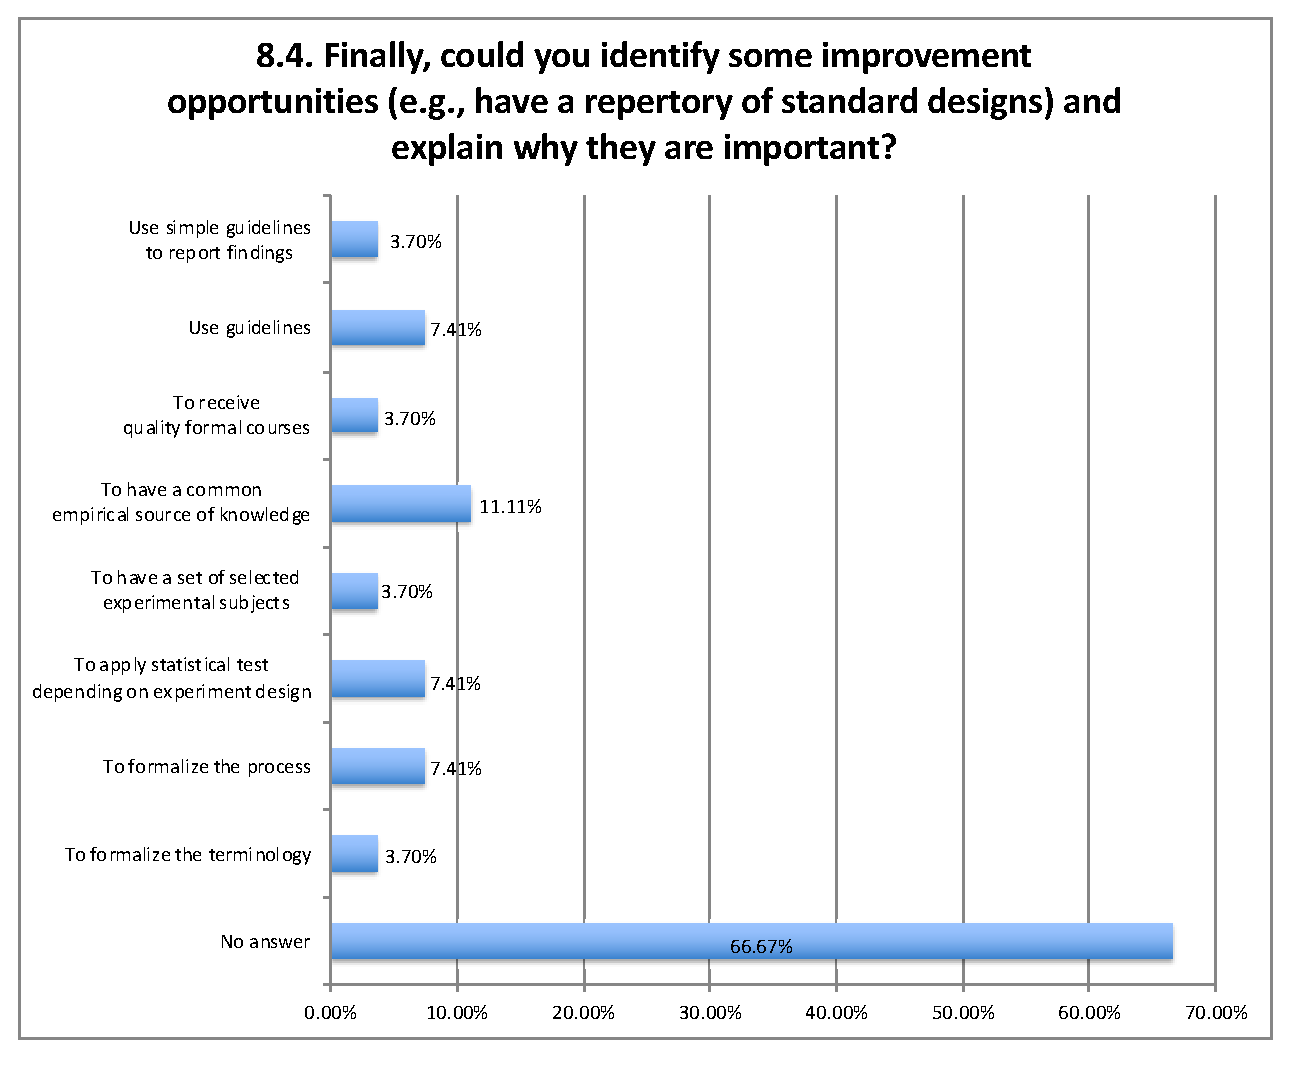
\includegraphics[width=12cm]{Images/Recommendations-Improve-SE-Experimentation}
	\caption{Recommendations to Improve the Experimentation in SE}
	\label{fig-recommendations-improve-SE-experimentation}
\end{figure*}



% Please add the following required packages to your document preamble:
% \usepackage{graphicx}
% \usepackage{lscape}
\begin{landscape}
\begin{table}[]
\centering
\resizebox{\textwidth}{!}{%
\begin{tabular}{rlll}
\hline
\# & Hallazgos del estudio en SE & Hallazgos del estudio en biotecnologia & \# \\ \hline
39 & Existe literatura est�ndar, e.g., \textbackslash{}cite\{Wohlin2000,Juristo2001\} &  &  \\
40 & La carencia de literatura est�ndar se suple con reportes o art�culos espec�ficos, e.g., \textbackslash{}cite\{Basili-1986-ESE\} &  &  \\
 2 & Se produce diversidad terminol�gica entre fuentes &  &  \\
 5 & Existen pocos libros de referencia acerca de experimentaci�n en SE &  &  \\
12 & No existe una pol�tica para la gesti�n del material, o herramientas especializadas &  &  \\
 &  &  & 
\end{tabular}%
}
\caption{Comparaci�n de los hallazgos en SE y Biotecnologia}
\label{tab:comparison}
\end{table}
\end{landscape}
%=========================


%\section{Introduction}
%\label{intro}
%Your text comes here. Separate text sections with
%\section{Section title}
%\label{sec:1}
%Text with citations \cite{RefB} and \cite{RefJ}.
%\subsection{Subsection title}
%\label{sec:2}
%as required. Don't forget to give each section
%and subsection a unique label (see Sect.~\ref{sec:1}).
%\paragraph{Paragraph headings} Use paragraph headings as needed.
%\begin{equation}
%a^2+b^2=c^2
%\end{equation}

% For one-column wide figures use
%\begin{figure}
% Use the relevant command to insert your figure file.
% For example, with the graphicx package use
%  
\includegraphics{example.eps}
% figure caption is below the figure
%\caption{Please write your figure caption here}
%\label{fig:1}       % Give a unique label
%\end{figure}
%
% For two-column wide figures use
%\begin{figure*}
% Use the relevant command to insert your figure file.
% For example, with the graphicx package use
%  
\includegraphics[width=0.75\textwidth]{example.eps}
% figure caption is below the figure
%\caption{Please write your figure caption here}
%\label{fig:2}       % Give a unique label
%\end{figure*}
%
% For tables use
%\begin{table}
% table caption is above the table
%\caption{Please write your table caption here}
%\label{tab:1}       % Give a unique label
% For LaTeX tables use
%\begin{tabular}{lll}
%\hline\noalign{\smallskip}
%first & second & third  \\
%\noalign{\smallskip}\hline\noalign{\smallskip}
%number & number & number \\
%number & number & number \\
%\noalign{\smallskip}\hline
%\end{tabular}
%\end{table}


%\begin{acknowledgements}
%Thanks et all.
%\end{acknowledgements}

% BibTeX users please use one of
%\bibliographystyle{spbasic}      % basic style, author-year citations
%\bibliographystyle{spmpsci}      % mathematics and physical sciences
%\bibliographystyle{spphys}       % APS-like style for physics
\bibliographystyle{ieeetr}
\bibliography{Biblio-Experimental-Process-SE} % name your BibTeX data base

% Non-BibTeX users please use
%\begin{thebibliography}{}
%
% and use \bibitem to create references. Consult the Instructions
% for authors for reference list style.
%
%\bibitem{RefJ}
% Format for Journal Reference
%Author, Article title, Journal, Volume, page numbers (year)
% Format for books
%\bibitem{RefB}
%Author, Book title, page numbers. Publisher, place (year)
% etc
%\end{thebibliography}

\clearpage
\onecolumn

\begin{appendices}

\appendixpage

\section{Conceptual models of Experimentation on SE}\label{sec:annex-models-SE}

Las figuras contienen t�rminos en Espa�ol, idioma en que se realiz� la investigaci�n. Hemos preferido no traducir las figuras para asegurar la trazabilidad entre en art�culo y la raw data, disponible en \url{}\odnote{RODRIGO: Indicar ubicaci�n de la raw data}.

\begin{figure*}[htbp!]
	\centering
	\captionsetup{justification=centering}
	
\includegraphics[width=\textwidth]{images/Producto-Intermedio-Revision-Lit}
	\caption{Modelo conceptual preliminar resultado del an�lisis de la literatura relevante.}
	\label{fig-conceptos-preliminar}
	\odnote{RODRIGO: He movido la figura a un anexo. Que se vea entera. D�jala en Espa�ol, ya que es posible que haya que haya que enlazar a ese ap�ndice el resto del row data de la tesis}
\end{figure*}

\begin{figure*}[htbp!]
	\centering
	
\includegraphics[width=5in]{images/Producto-Final-Revision-Lit}
	\caption{Modelo conceptual resultado del an�lisis de los materiales experimentales.}
	\label{fig-conceptos-final-revision-fuentes}\odnote{RODRIGO: Pon el modelo completo.}
\end{figure*}

%\begin{figure*}[htbp!]
%	\centering
%	\includegraphics[width=5in]{images/Producto-Final-Observacion-Par}
%	\caption{Modelo conceptual resultado de la observaci�n participativa.}
%	\label{fig-conceptos-final-observacion-participativa}\odnote{RODRIGO: Hay que crear esta figura.}
%\end{figure*}

%\begin{figure*}[htbp!]
	%\centering
	%\includegraphics[width=5in]{images/Model}
	%\caption{Modelo conceptual resultado de las entrevistas semi-estructuradas.}
	%\label{fig-modelo-exp}\odnote{RODRIGO: Hay que crear esta figura.}
%\end{figure*}

%\begin{sidewaysfigure}%[htbp!]
%	\centering
%	\includegraphics[width=28cm]{images/Final-Proccess-Workflow}
%	\caption{Workflow del proceso de experimentaci�n en SE resultado de las entrevistas semi-estructuradas.}
%	\label{fig-final-process-workflow}
%\end{sidewaysfigure}

\begin{figure}[htbp!]
	\centering
	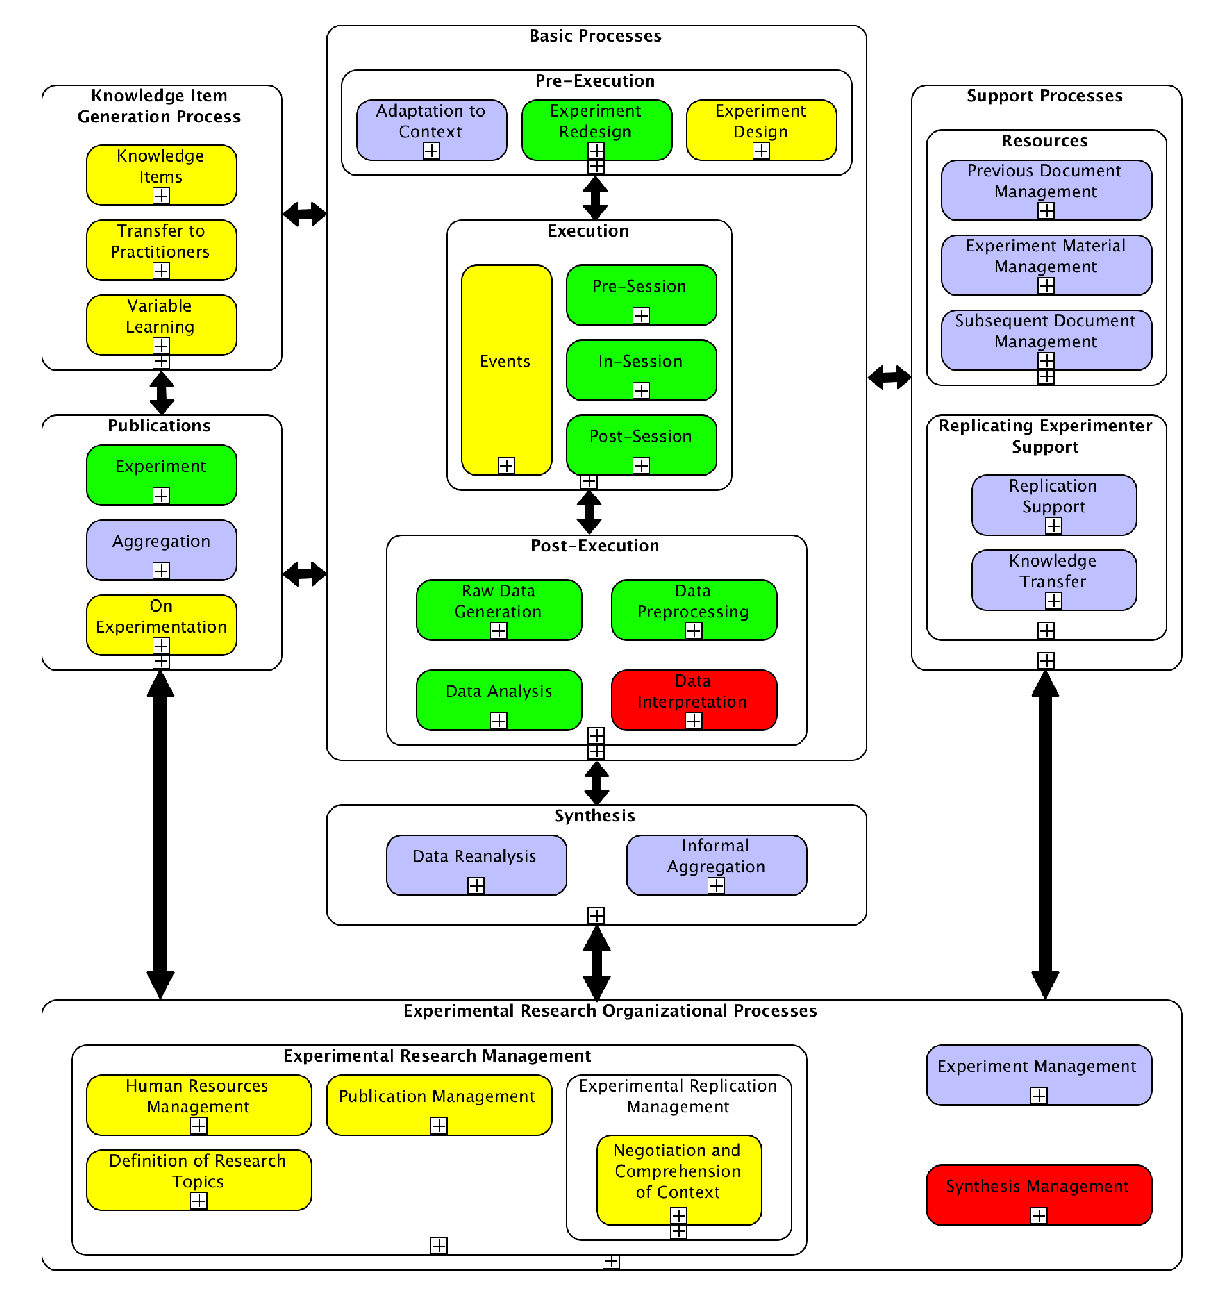
\includegraphics[width=18cm]{Images/Final-Experimentation-Process-Model}
	\caption{Modelo del proceso de experimentaci�n en SE resultado de las entrevistas semi-estructuradas.}
	\label{fig-final-process-model}
\end{figure}

\begin{sidewaysfigure}%[htbp!]
	\centering
	\includegraphics[width=28cm]{Images/Conceptual-Model-RM}
	\caption{SE Conceptual Model From Research Manager Point Of View}
	\label{fig-conceptual-model-RM}
\end{sidewaysfigure}

\begin{sidewaysfigure}%[htbp!]
	\centering
	\includegraphics[width=28cm]{Images/Conceptual-Model-EM}
	\caption{SE Conceptual Model From Experiment Manager Point Of View}
	\label{fig-conceptual-model-EM}
\end{sidewaysfigure}

\begin{sidewaysfigure}%[htbp!]
	\centering
	\includegraphics[width=28cm]{Images/Conceptual-Model-SE}
	\caption{SE Conceptual Model From Senior Experimenter Point Of View}
	\label{fig-conceptual-model-SE}
\end{sidewaysfigure}


\section{Conceptual models of Experimentation on Biotechnology}\label{sec:annex-models-BIO}

\begin{figure}[htbp!]
	\centering
	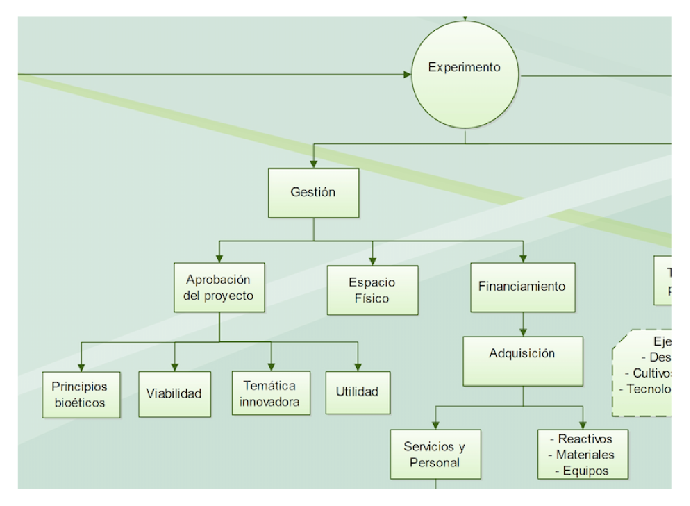
\includegraphics[width=3in]{Images/Concepts-Draft-Bio}
	\caption{Modelo Conceptual Inicial de Biotecnolog�a}
	\label{fig-concepts-initial-bio}\odnote{RODRIGO: Poner modelo completo}.
\end{figure}

\begin{figure}[htbp!]
	\centering
	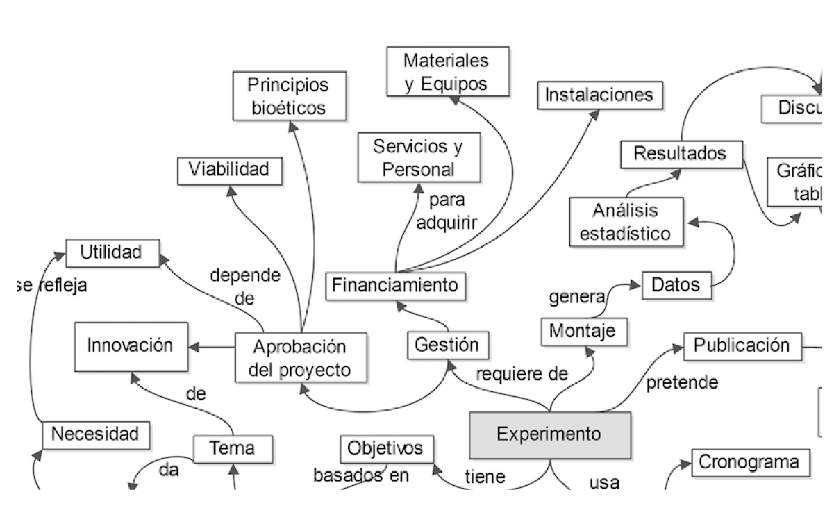
\includegraphics[width=3in]{Images/Concepts-Final-Bio}
	\caption{Modelo Conceptual final de experimentaci�n en Biotecnolog�a}
	\label{fig-concepts-final-bio}\odnote{RODRIGO: Poner modelo completo}.
\end{figure}

\begin{figure}[htbp!]
	\centering
	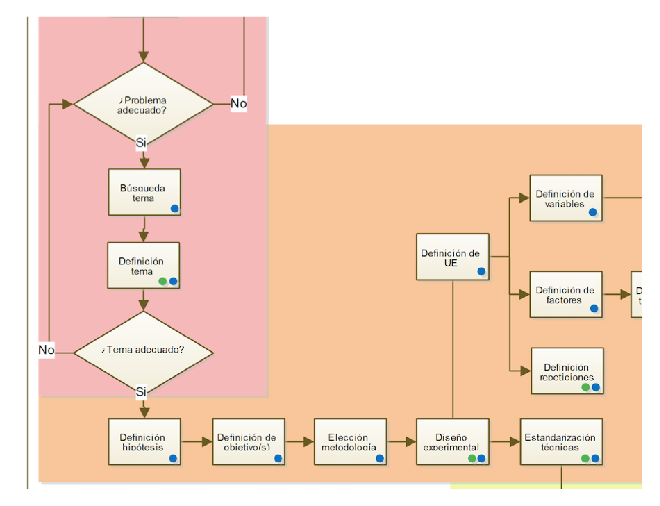
\includegraphics[width=3.2in]{Images/Final-Process}
	\caption{Modelo final del proceso experimental en Biotecnolog�a}
	\label{fig-proceso-exp-final}\odnote{RODRIGO: Poner modelo completo}.
\end{figure}

\end{appendices}

\end{document}
% end of file template.tex

